%\documentclass[gray,handout, pdftex, 11pt]{beamer}
%\documentclass[handout, pdftex, 11pt]{beamer}
\documentclass[pdftex, 11pt]{beamer}

\usepackage{pgfpages}
\usepackage[utf8]{inputenc}
\usepackage[T1]{fontenc}
\usepackage{lmodern}
%\usepackage[italian]{babel}
\usepackage{graphicx}
\usepackage{microtype}
\usepackage{acronym}
\usepackage{array}
%\usepackage{natbib}
\usepackage{verbatim}
\usepackage{appendixnumberbeamer}
%\usepackage{advdate}
\usepackage{color}
\usepackage{multirow}

\usepackage{tikz}
\usetikzlibrary{intersections, arrows, shapes, decorations.pathreplacing, decorations.pathmorphing, calc}

%\AdvanceDate[1]

\definecolor{darkgreen}{rgb}{0.01, 0.75, 0.24}

\newcolumntype{C}[1]{>{\centering\let\newline\\\arraybackslash\hspace{0pt}}m{#1}}
\newcommand{\cellwidth}{1.2cm}
\newcommand{\svntitlesize}{\tiny}
\newcommand{\svnbodysize}{\tiny}

\newcommand{\cell}[2][c]{%
  \begin{tabular}[#1]{@{}c@{}}#2\end{tabular}}
\newcommand{\rowhead}[2]{\cell{\color{red}#1\\ \color{darkgreen}#2}}
\newcommand{\rowheadb}[3]{\cell{#1\\ \color{red}#2\\ #3}}
\newcommand{\cont}[5]{\cell{\color{red}#1\\ \color{blue}#2\\ #3\\ #4\\ \color{darkgreen}#5}}
\newcommand{\deprecont}[5]{\cell{\color{red}#1\\ \color{blue}#2\\ #3\\ #4\\ \color{darkgreen}#5\\ \color{red}Deprecated warning}}
\newcommand{\noacc}{No accumulation}
\newcommand{\acc}{Accumulation}
\newcommand{\noconv}{No conversion}
\newcommand{\sca}{Scaling possible}
\newcommand{\nosca}{Scaling not possible}
\newcommand{\conv}{Conversion}
\newcommand{\module}{\color{red}Module}
\newcommand{\rod}{\color{red}Rod}
\newcommand{\layer}{\color{red}Layer/Disk}
\newcommand{\serfal}{\color{darkgreen}Service=false}
\newcommand{\sertru}{\color{darkgreen}Service=true}
\newcommand{\err}{\color{red}Error}
\newcommand{\depre}{\color{red}Deprecated}
\newcommand{\follsup}{Following supports $S_{R+1}\dots S_i\dots S_N$}
\newcommand{\allsup}{All supports $S_1\dots S_i\dots S_N$}
\newcommand{\modlen}{moduleLength}
\newcommand{\modsur}{moduleSurface}
\newcommand{\nummod}{numModules}
\newcommand{\suplen}{supportLength}
\newcommand{\supsur}{supportSurface}
\newcommand{\mapbar}{\color{red}Barrel}
\newcommand{\mapen}{\color{red}Endcap}


\mode<presentation>{
  %-------------------------1
  \usetheme{Boadilla}
  \usecolortheme{beaver}
  %-------------------------1
  %-------------------------2
  %\usetheme{Goettingen}
  %\usecolortheme{sidebartab}
  %-------------------------2
  %\useoutertheme[right]{sidebar}
  %\usefonttheme{default}
  \setbeamercovered{transparent}
  %\setbeameroption{show notes on second screen=right}
  \setbeamertemplate{navigation symbols}{}

  \bibliographystyle{abbrv}  
  %\renewcommand\bibfont{\scriptsize}
  \setbeamertemplate{bibliography item}{\textbullet}
  \setbeamertemplate{itemize item}{\checkmark}
  \setbeamertemplate{itemize subitem}{-}
  \setbeamertemplate{enumerate items}[default]
  \setbeamertemplate{sections/subsections in toc}[square]
}

\title[Material testing]{\textbf{MATERIAL TESTING}}
\subtitle{tkLayout developers meeting}
\institute[CERN]{
  %{\Large\textbf{CERN}}\\{European Organization for Nuclear Research}\\[0.5cm]
  %\\[0.2cm]
  European Organization for Nuclear Research\\[0.5cm]
  
\includegraphics[width=2cm]{img/LogoBadge.pdf}\\
}

\author[Stefano Martina]{
  %\\[0.2cm]
  \textbf{Stefano MARTINA}\\
  {\small stefano.martina@cern.ch}
}

\date[\today]{\flushright \today}

\begin{document}

\begin{frame}[plain,noframenumbering]
  \titlepage
\end{frame}

\begin{frame}{Testing algorithm}
  \begin{enumerate}
  \item Build test case with controlled amount of material
  \item Get elements \alert{coordinates}
    \begin{itemize}
    \item [$\to$] from tklayout run
    \end{itemize}
  \item Build model with \alert{expected} material in each element
  \item \alert{Calculate} thickness in radiation length
  \item \alert{Correlate} tklayout \alert{output} with \alert{expected} calculation
  \end{enumerate}
\end{frame}

\begin{frame}
  \fontsize{4.5pt}{6pt}\selectfont
  \begin{center}
    \begin{tabular}{|c|c|c|c|}
      \cline{2-4}
      \multicolumn{1}{c|}{} & \color{darkgreen}Unit=$g/m$ & \color{darkgreen}Unit=$mm$ & \color{darkgreen}Unit=$g$\\
      \hline
      \rowhead{\module}{\serfal} & \cont{\module}{$\times \modlen$}{\noacc}{\noconv}{\sca}& \cont{\module}{$\times \modsur\times \rho$ (sensor surface)}{\noacc}{\noconv}{\sca}& \cont{\module}{$\times 1$}{\noacc}{\noconv}{\sca}\\
      \hline
      \rowheadb{\module}{ring $R$ of $N$}{\sertru} & \cont{\follsup}{$\times \nummod_R \times \suplen_i$}{\acc}{\conv (1:1 by default, with warning)}{\sca} & \deprecont{\follsup}{$\times \nummod_R \times \supsur_i \times \rho$}{\acc}{\conv  (1:1 by default, with warning)}{\sca} & \err \\
      \hline
      \rowhead{\rod (barrel)}{\serfal} & \cont{\allsup}{$\times \nummod_1 \times \suplen_i$}{\noacc}{\noconv}{\nosca} & \cont{\allsup}{$\times \supsur_i \times \rho$}{\noacc}{\noconv}{\nosca} & \cont{\allsup}{$\times \nummod_1 \times \frac{\suplen_i}{\sum_{j=1}^N\suplen_j}$}{\noacc}{\noconv}{\nosca} \\
      \hline
      \rowhead{\rod (barrel)}{\sertru} & \cont{\allsup}{$\times \nummod_1 \times \suplen_i$}{\noacc}{\conv}{\nosca} & \deprecont{\allsup}{$\times \supsur_i \times \rho$}{\noacc}{\conv}{\nosca} & \err \\
      \hline
      \rowhead{\layer}{\serfal} & \cont{\allsup}{$\times \suplen_i$}{\noacc}{\noconv}{\nosca} & \cont{\allsup}{$\times \supsur_i \times \rho$}{\noacc}{\noconv}{\nosca} & \cont{\allsup}{$\times \frac{\suplen_i}{\sum_{j=1}^N\suplen_j}$}{\noacc}{\noconv}{\nosca} \\
      \hline
      \rowhead{\layer}{\sertru} & \cont{\allsup}{$\times \suplen_i$}{\noacc}{\conv}{\nosca} & \deprecont{\allsup}{$\times \supsur_i \times \rho$}{\noacc}{\conv}{\nosca} & \err \\
      \hline
    \end{tabular}
  \end{center}
\end{frame}

\begin{frame}{Compute expected material for \emph{g/m} unit}
  \begin{block}{Cylinder, \alert{$L$} $g/m$ of material \alert{M}}
    $$
    \frac{X_0}{X_{0M}} = \frac{L/1000}{2\pi r \cdot X_{0M}} \cdot \frac{e^\eta+e^{-\eta}}{2}
    $$
  \end{block}
  \begin{block}{Disk, \alert{L} $g/m$ of material \alert{M}}
    $$
    \frac{X_0}{X_{0M}} = \frac{L/1000}{\pi(r_1+r_2)\cdot X_{0M}}\cdot\frac{e^{2\eta}+1}{e^{2\eta}-1}
    $$
  \end{block}

  \begin{itemize}
  \item For \alert{layers} rods, \alert{$L$} is:
    \begin{itemize}
    \item [$\to$] the set material multiplied by the number of rods
    \end{itemize}
  \item For \alert{disks} ``rods'', \alert{$L$} is:
    \begin{itemize}
    \item [$\to$] the set material multiplied by the number of modules of the first ring
    \end{itemize}
  \end{itemize}
\end{frame}

\begin{frame}{Compute expected material for \emph{mm} unit}
  \begin{block}{Cylinder, \alert{$L$} $mm$ of material \alert{M}}
    $$
    \frac{X_0}{X_{0M}} = \frac{L\cdot\rho_M}{X_{0M}}\cdot\frac{e^\eta+e^{-\eta}}{2}
    $$
  \end{block}
  \begin{block}{Disk, \alert{$L$} $mm$ of material \alert{M}}
    $$
    \frac{X_0}{X_{0M}} = \frac{L\cdot\rho_M}{X_{0M}}\cdot\frac{e^{2\eta}+1}{e^{2\eta}-1}
    $$
  \end{block}

  \begin{itemize}
  \item For \alert{layers} and \alert{disks} rods, \alert{$L$} is:
    \begin{itemize}
    \item[$\to$] the set material (not replicated for rod or modules)
    \end{itemize}
  \end{itemize}
\end{frame}

\begin{frame}{Compute expected material for \emph{g} unit}
  \begin{block}{Cylinder, \alert{$L$} $g$ of material \alert{M}}
    $$
    \frac{X_0}{X_{0M}} = \frac{L}{2\pi r (z_2-z_1) \cdot X_{0M}} \cdot \frac{e^\eta+e^{-\eta}}{2}
    $$
  \end{block}
  \begin{block}{Disk, \alert{L} $g$ of material \alert{M}}
    $$
    \frac{X_0}{X_{0M}} = \frac{L}{\pi(r_2^2-r_1^2)\cdot X_{0M}}\cdot\frac{e^{2\eta}+1}{e^{2\eta}-1}
    $$
  \end{block}
  \begin{itemize}
  \item Unit \alert{g} can't be used for rods in layers and disks
  \end{itemize}
\end{frame}

\begin{frame}{Compute expected material for one barrel module \alert{$m$}}
  \begin{block}{Equivalent \alert{g/m} cylinder \alert{$c$}}
    $$
    L_c = \frac{L_m}{w}\cdot 2\pi r
    $$
  \end{block}

  \begin{block}{Equivalent \alert{mm} cylinder \alert{$c$}}
    $$
    L_c = L_m
    $$
  \end{block}

  \begin{block}{Equivalent \alert{g} cylinder \alert{$c$}}
    $$
    L_c = \frac{L_m}{w}\cdot 2\pi r
    $$
  \end{block}

  \begin{itemize}
  \item $c$ is the middle longitudinal segment of $m$ rotated in $\varphi$
  \item valid analysis if track gun at fixed $\varphi$
  \item $w = $ module width
  \end{itemize}
\end{frame}

\begin{frame}{Compute expected material for one endcap module \alert{$m$}}
  \begin{block}{Equivalent \alert{g/m} disk \alert{$d$}}
    $$
    L_d = \frac{L_m}{w}\cdot \pi (r_1 + r_2)
    $$
  \end{block}

  \begin{block}{Equivalent \alert{mm} disk \alert{$d$}}
    $$
    L_d = L_m
    $$
  \end{block}

  \begin{block}{Equivalent \alert{g} disk \alert{$d$}}
    $$
    L_d = \frac{L_m}{w}\cdot \pi (r_1 + r_2)
    $$
  \end{block}

  \begin{itemize}
  \item $d$ is the middle longitudinal segment of $m$ rotated in $\varphi$
  \item valid analysis if track gun at fixed $\varphi$
  \item $w = $ module width
  \end{itemize}
\end{frame}

\begin{frame}{Tests map}
  \fontsize{5.5pt}{8.5}\selectfont
  %\begin{savenotes}
    \begin{center}
      \begin{tabular}{|c|c|C{\cellwidth}|C{\cellwidth}|C{\cellwidth}|C{\cellwidth}|C{\cellwidth}|C{\cellwidth}|}
        \cline{3-8}
        \multicolumn{2}{c|}{} & \multicolumn{2}{c|}{\color{darkgreen}Unit=$g/m$ (linear dens.)} & \multicolumn{2}{c|}{\color{darkgreen}Unit=$mm$ (thickness)} & \multicolumn{2}{c|}{\color{darkgreen}Unit=$g$ (weight)}\\
        \cline{3-8}
        \multicolumn{2}{c|}{} & \serfal & \sertru & \serfal & \sertru & \serfal & \sertru \\
        \hline
        \multirow{2}{*}{\module} & \mapbar & test22\footnote{\label{equivnote}Studied blocking track gun at $\pi/2$ and converting in equivalent cylinder/disk} & test4, test5 & test23\textsuperscript{\ref{equivnote}} & test13b & test24\textsuperscript{\ref{equivnote}} & \err \\
        \cline{2-8}
        & \mapen & test22d\textsuperscript{\ref{equivnote}} & test6bis, test14 & test23d\textsuperscript{\ref{equivnote}} & test13 & test24d\textsuperscript{\ref{equivnote}} & \err \\
        \hline
        \multirow{2}{*}{\rod} & \mapbar & test20 & test1a, test1b, test1c, test1d, test2, test5, test7\footnote{\label{convnote}Test conversions}, test8\textsuperscript{\ref{convnote}}, test9\textsuperscript{\ref{convnote}}, test10\textsuperscript{\ref{convnote}}, test10bis\textsuperscript{\ref{convnote}}, test10ter\textsuperscript{\ref{convnote}}, test11\footnote{\label{scanote}Test scaling}, test11bis\textsuperscript{\ref{scanote}} & test3bis, test3ter & test3, test3quater & test21 & \err \\
        \cline{2-8}
        & \mapen & \err & \err & \err & \err & \err & \err \\
        \hline
        \multirow{2}{*}{\layer} & \mapbar & test19 & test19bis & test18 & test18bis & test17 & \err \\
        \cline{2-8}
        & \mapen & test15bis & test6, test15 & test12bis & test12  & test16 & \err \\
        \hline
      \end{tabular}
    \end{center}
  %\end{savenotes}
\end{frame}

\begin{frame}
  \begin{block}{Test1a}
    \alert{$100 g/m$} of \emph{Cu} in the rods of the first layer of the pixel barrel
    \begin{itemize}
    \item \alert{12} rods
    \item \alert{$L=1200$} for every element
    \end{itemize}
  \end{block}
  \begin{center}
    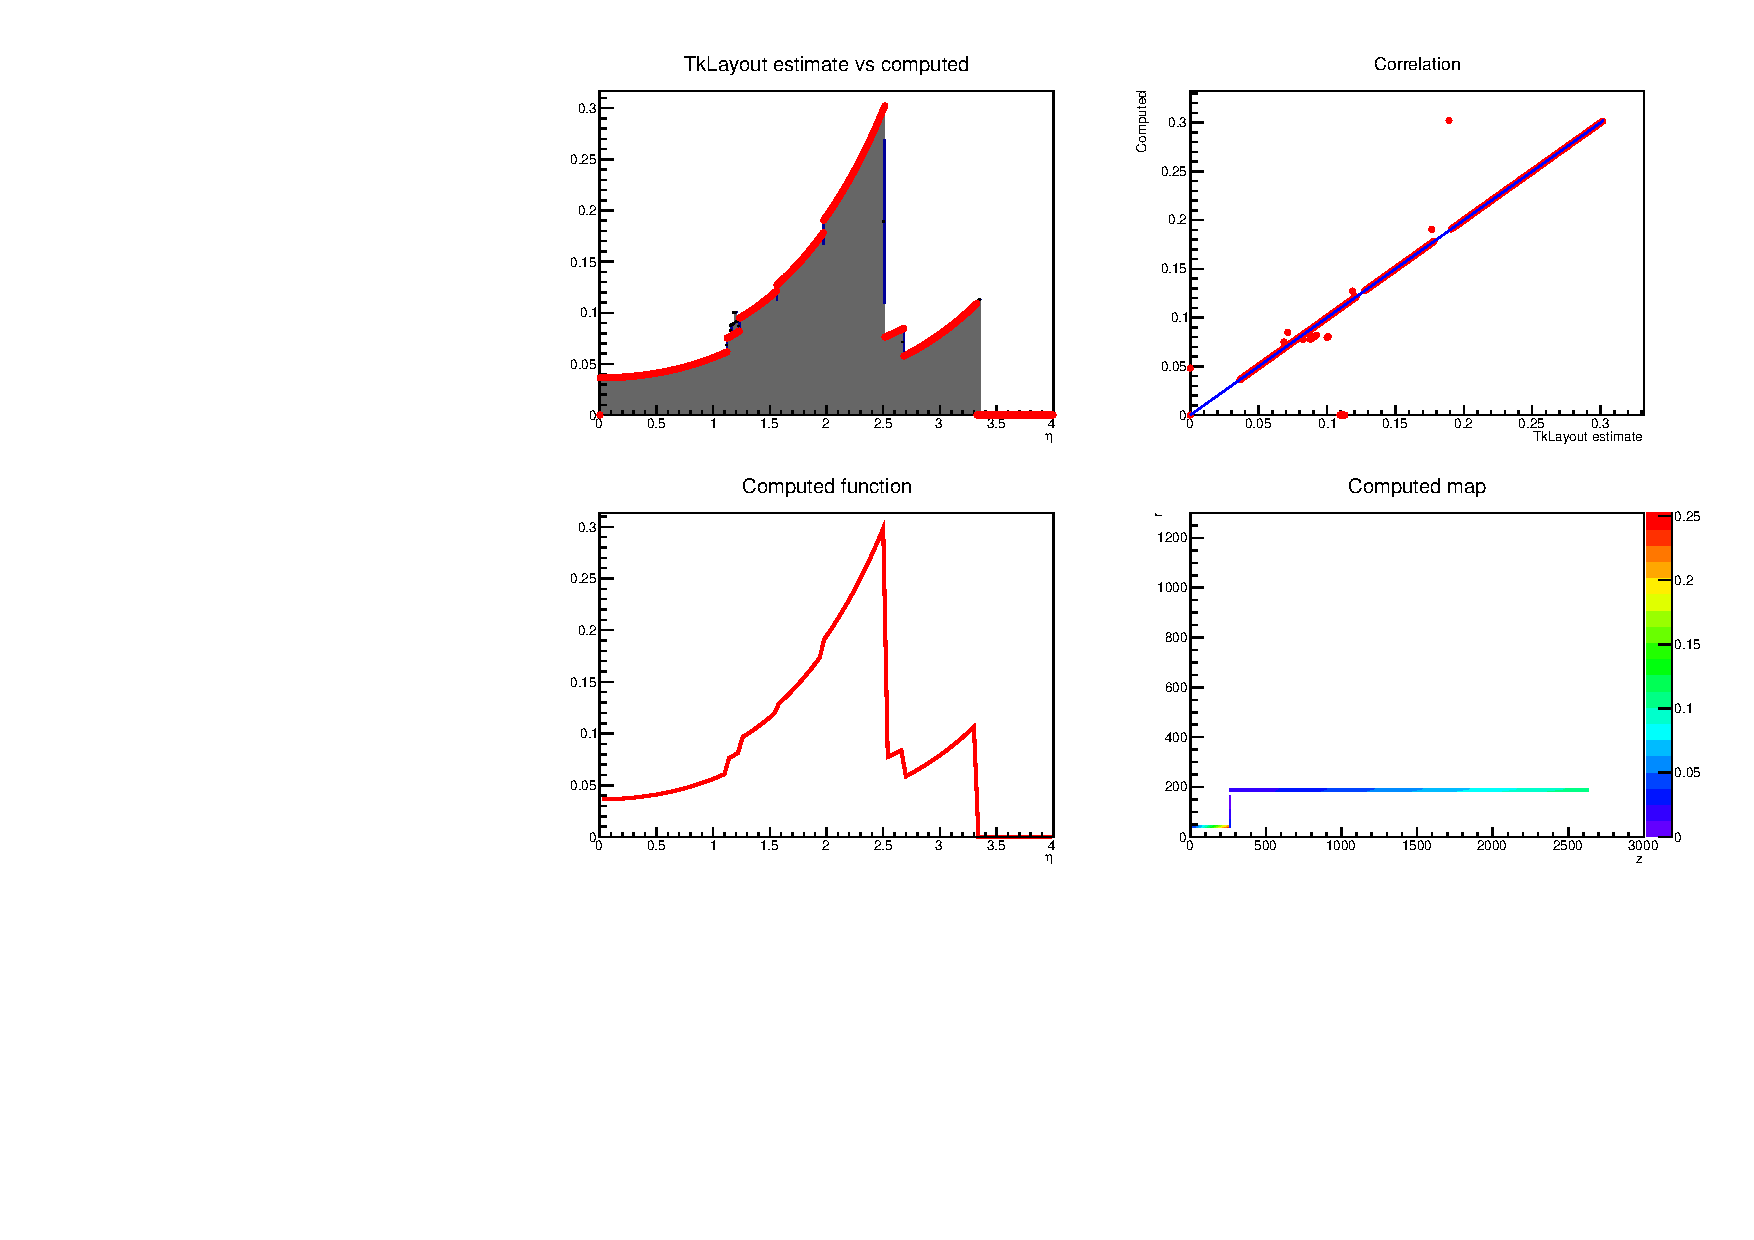
\includegraphics[width=9cm]{img/test1a.pdf}
  \end{center}
\end{frame}

\begin{frame}
  \begin{block}{Test1b}
    \alert{$100 g/m$} of \emph{Cu}  in the rods of the second layer of the pixel barrel
    \begin{itemize}
    \item \alert{24} rods
    \item \alert{$L=2400$} for every element
    \end{itemize}
  \end{block}
  \begin{center}
    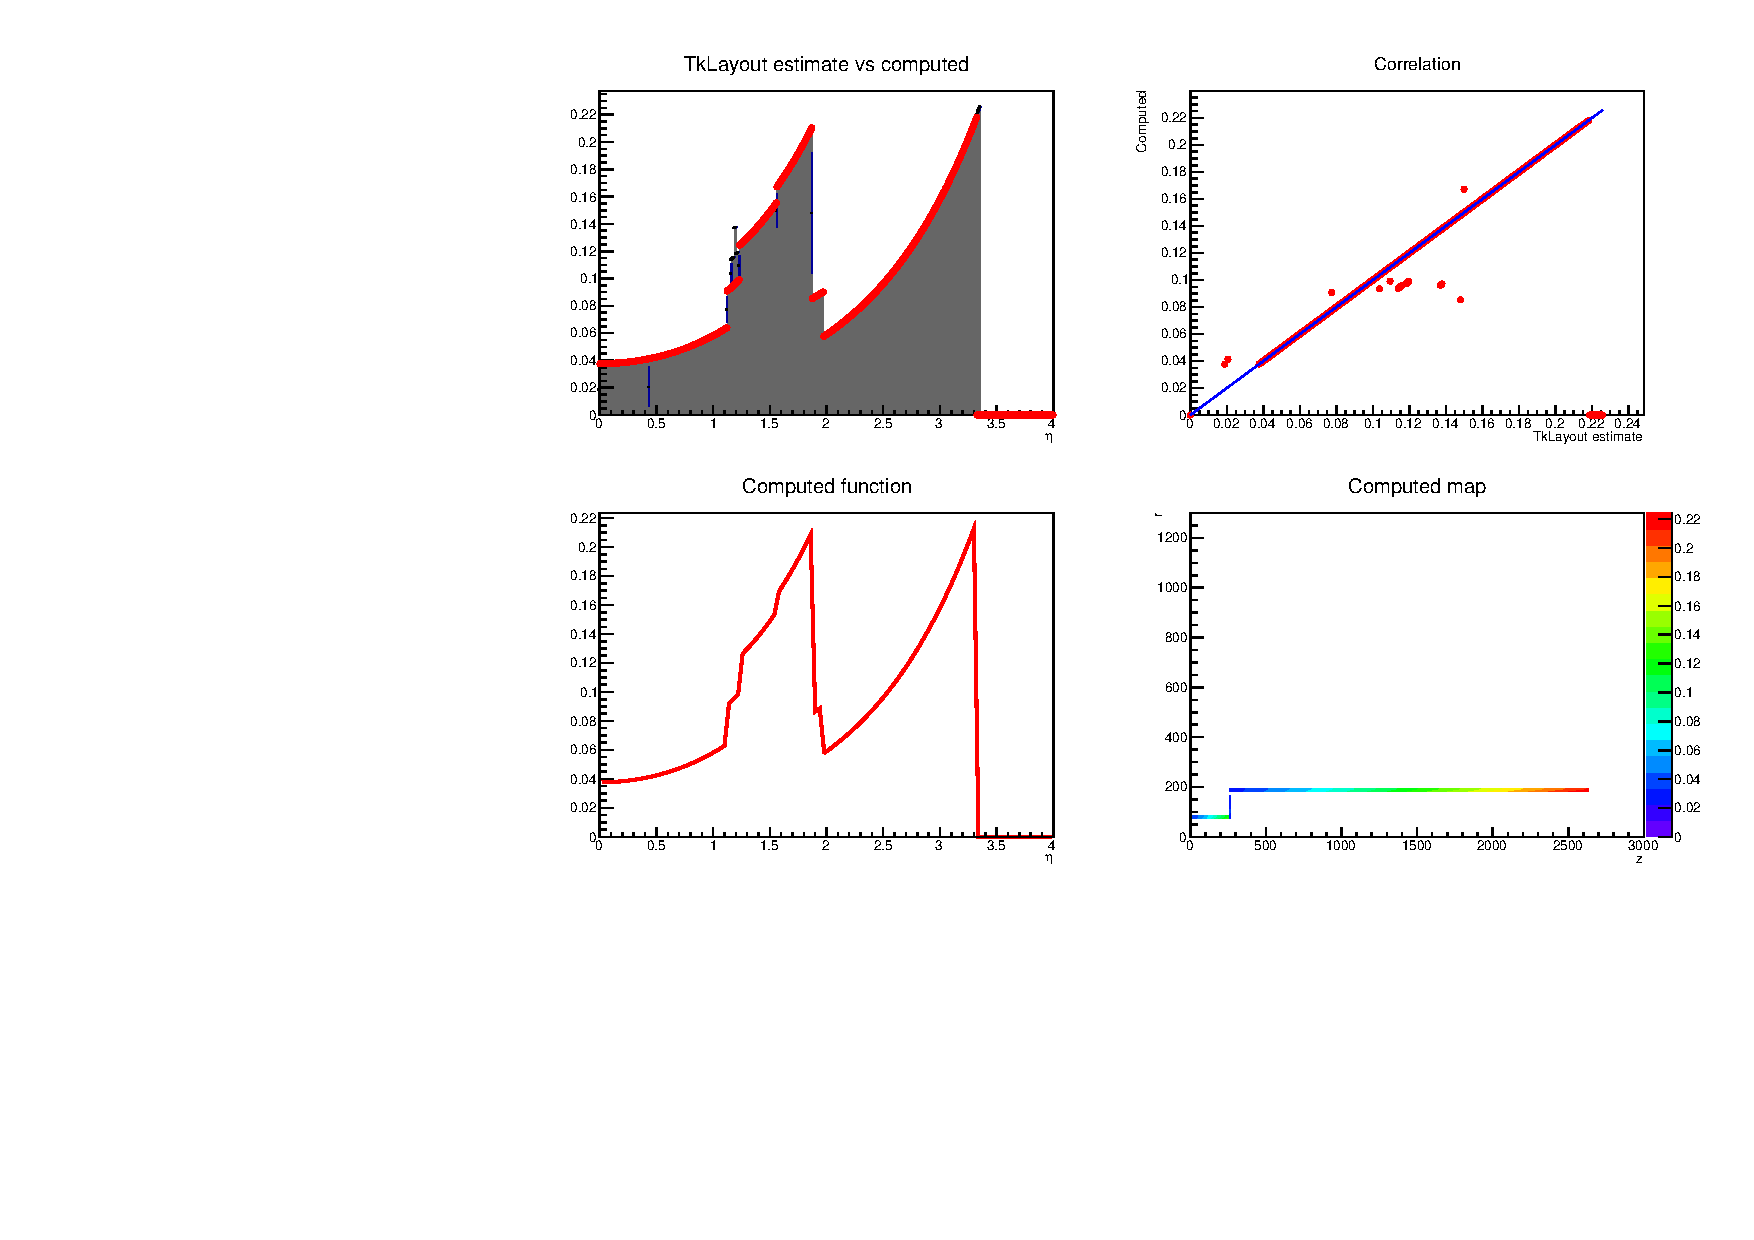
\includegraphics[width=9cm]{img/test1b.pdf}
  \end{center}
\end{frame}

\begin{frame}
  \begin{block}{Test1c}
    \alert{$100 g/m$} of \emph{Cu}  in the rods of the third layer of the pixel barrel
    \begin{itemize}
    \item \alert{36} rods
    \item \alert{$L=3600$} for every element
    \end{itemize}
  \end{block}
  \begin{center}
    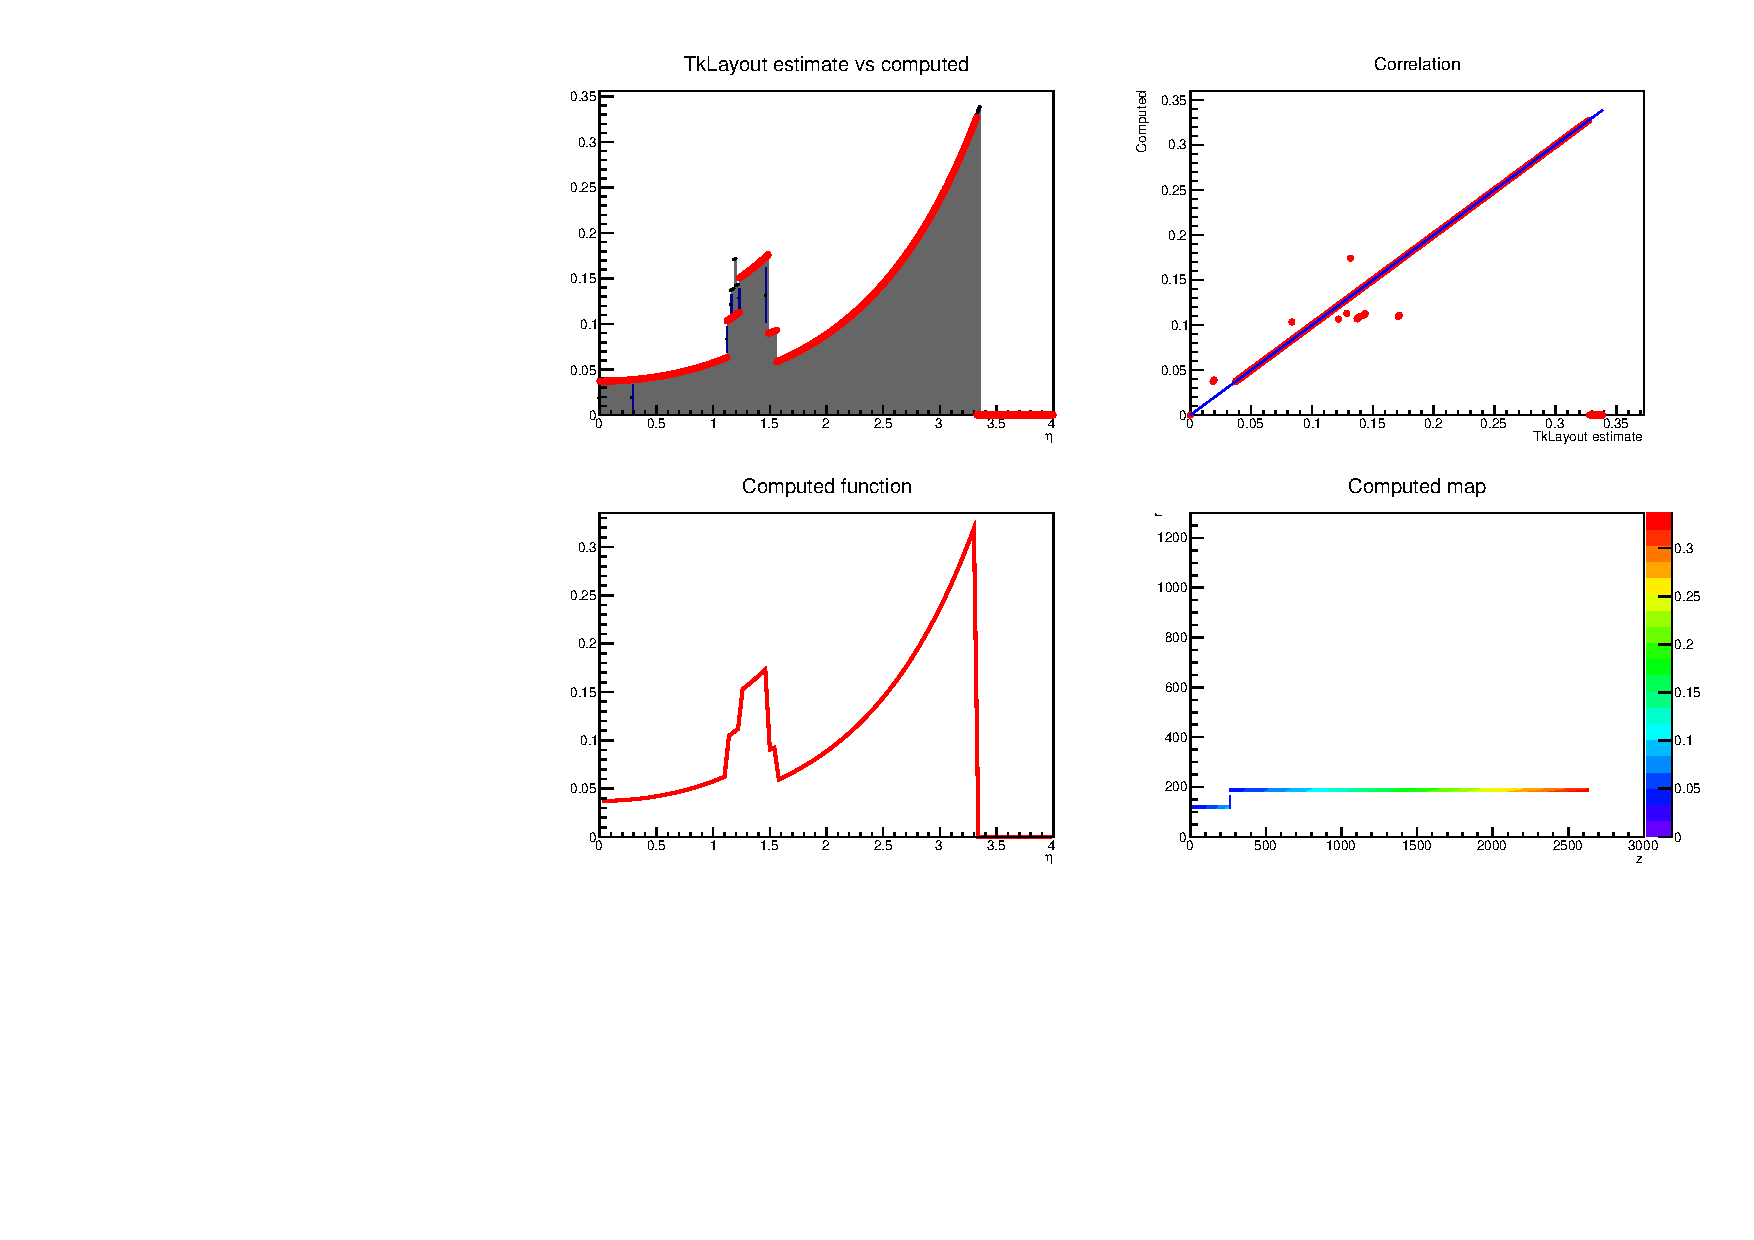
\includegraphics[width=9cm]{img/test1c.pdf}
  \end{center}
\end{frame}

\begin{frame}
  \begin{block}{Test1d}
    \alert{$100 g/m$} of \emph{Cu}  in the rods of the fourth layer of the pixel barrel
    \begin{itemize}
    \item \alert{52} rods
    \item \alert{$L=5200$} for every element
    \end{itemize}
  \end{block}
  \begin{center}
    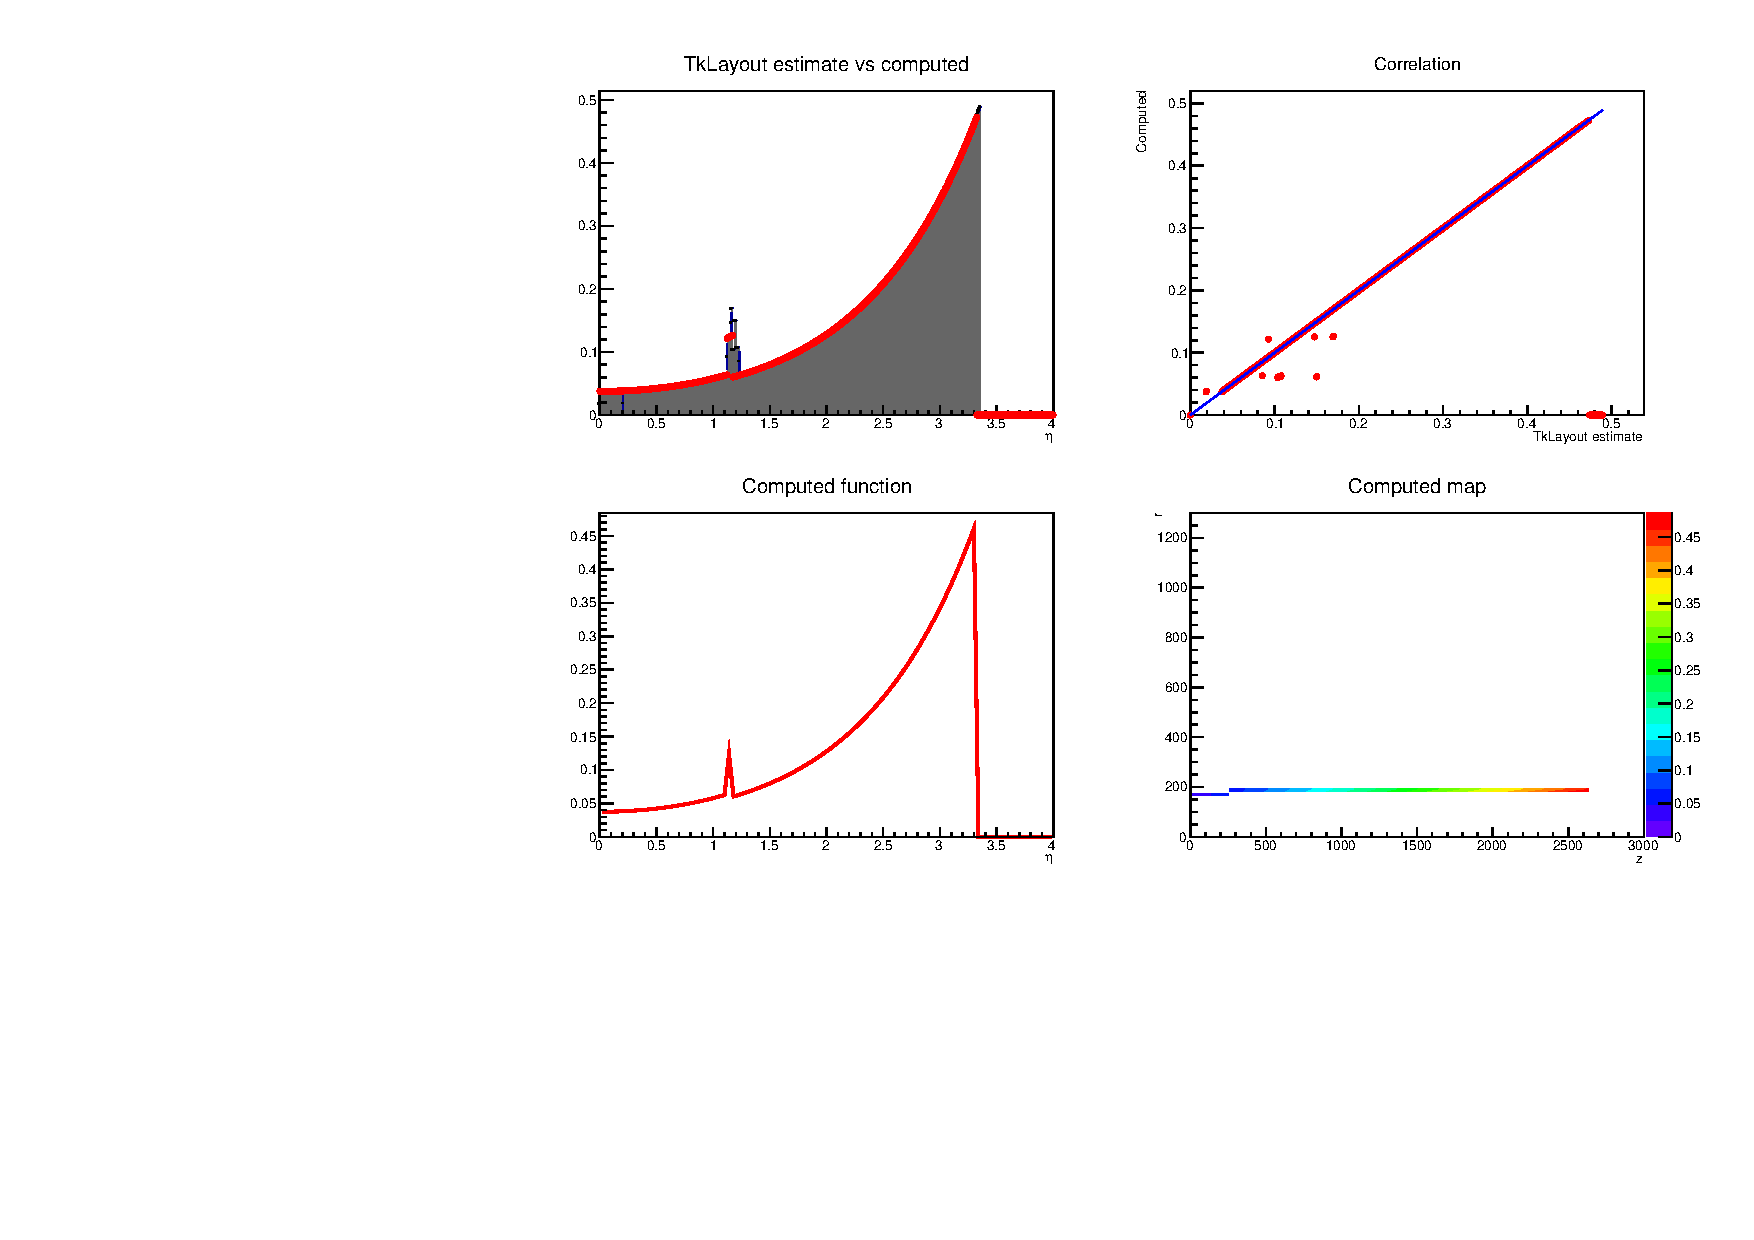
\includegraphics[width=9cm]{img/test1d.pdf}
  \end{center}
\end{frame}

\begin{frame}
  \begin{block}{Test2}
    \alert{$100 g/m$} of \emph{Cu}  in the rods of all the layers of the pixel barrel
    \begin{itemize}
    \item \alert{$L=rods*100$} for layers
    \item \alert{$L=L_{inLayer}+L_{inDisk}$} for disks and last cylinder
    \end{itemize}
  \end{block}
  \begin{center}
    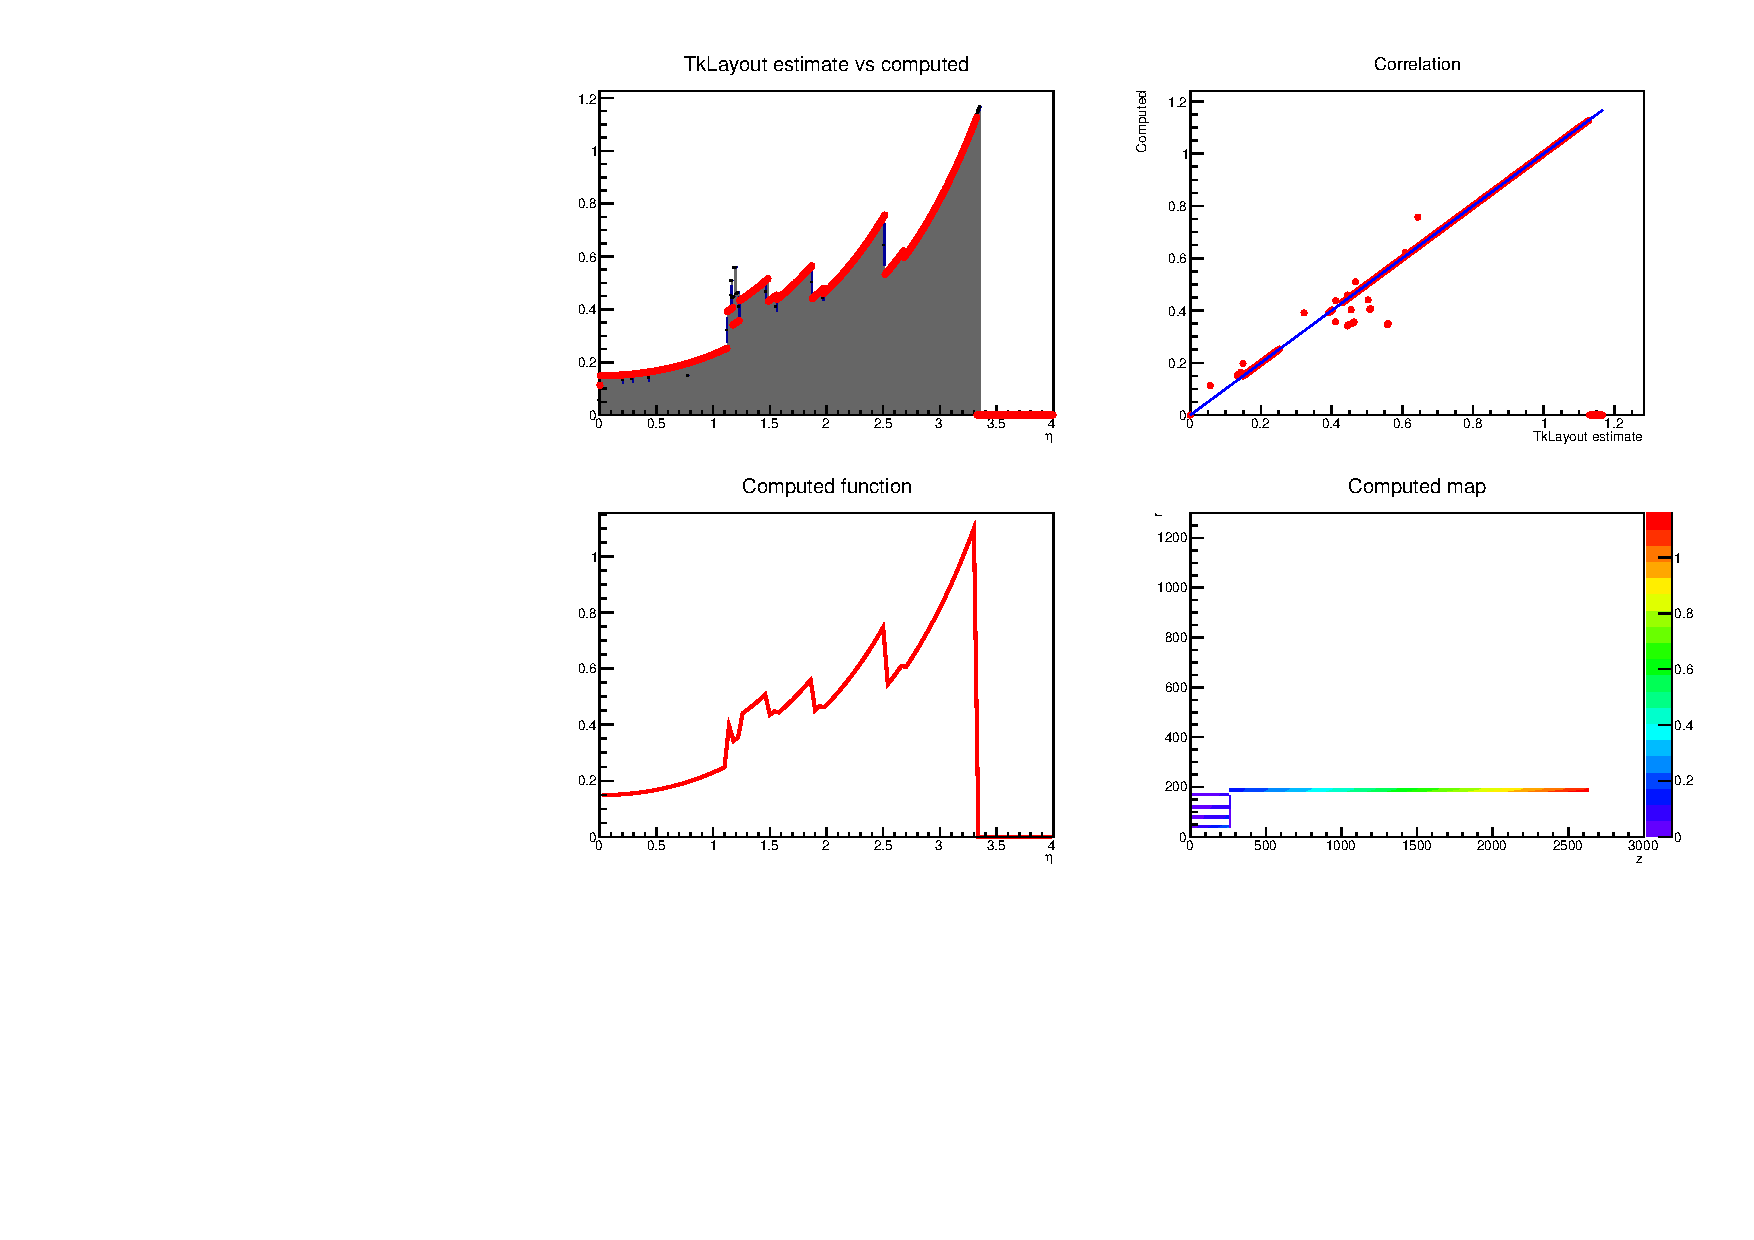
\includegraphics[width=9cm]{img/test2.pdf}
  \end{center}
\end{frame}

\begin{frame}
  \begin{block}{Test3}
    \alert{$0.1 mm$} of \emph{Cu}  in the rods of all the layers of the pixel barrel, exiting
    \begin{itemize}
    \item \alert{$L=0.1$} for layers
    \item \alert{$L=L_{inLayer}+L_{inDisk}$} for disks and last cylinder (\alert{deprecated feature})
    \end{itemize}
  \end{block}
  \begin{center}
    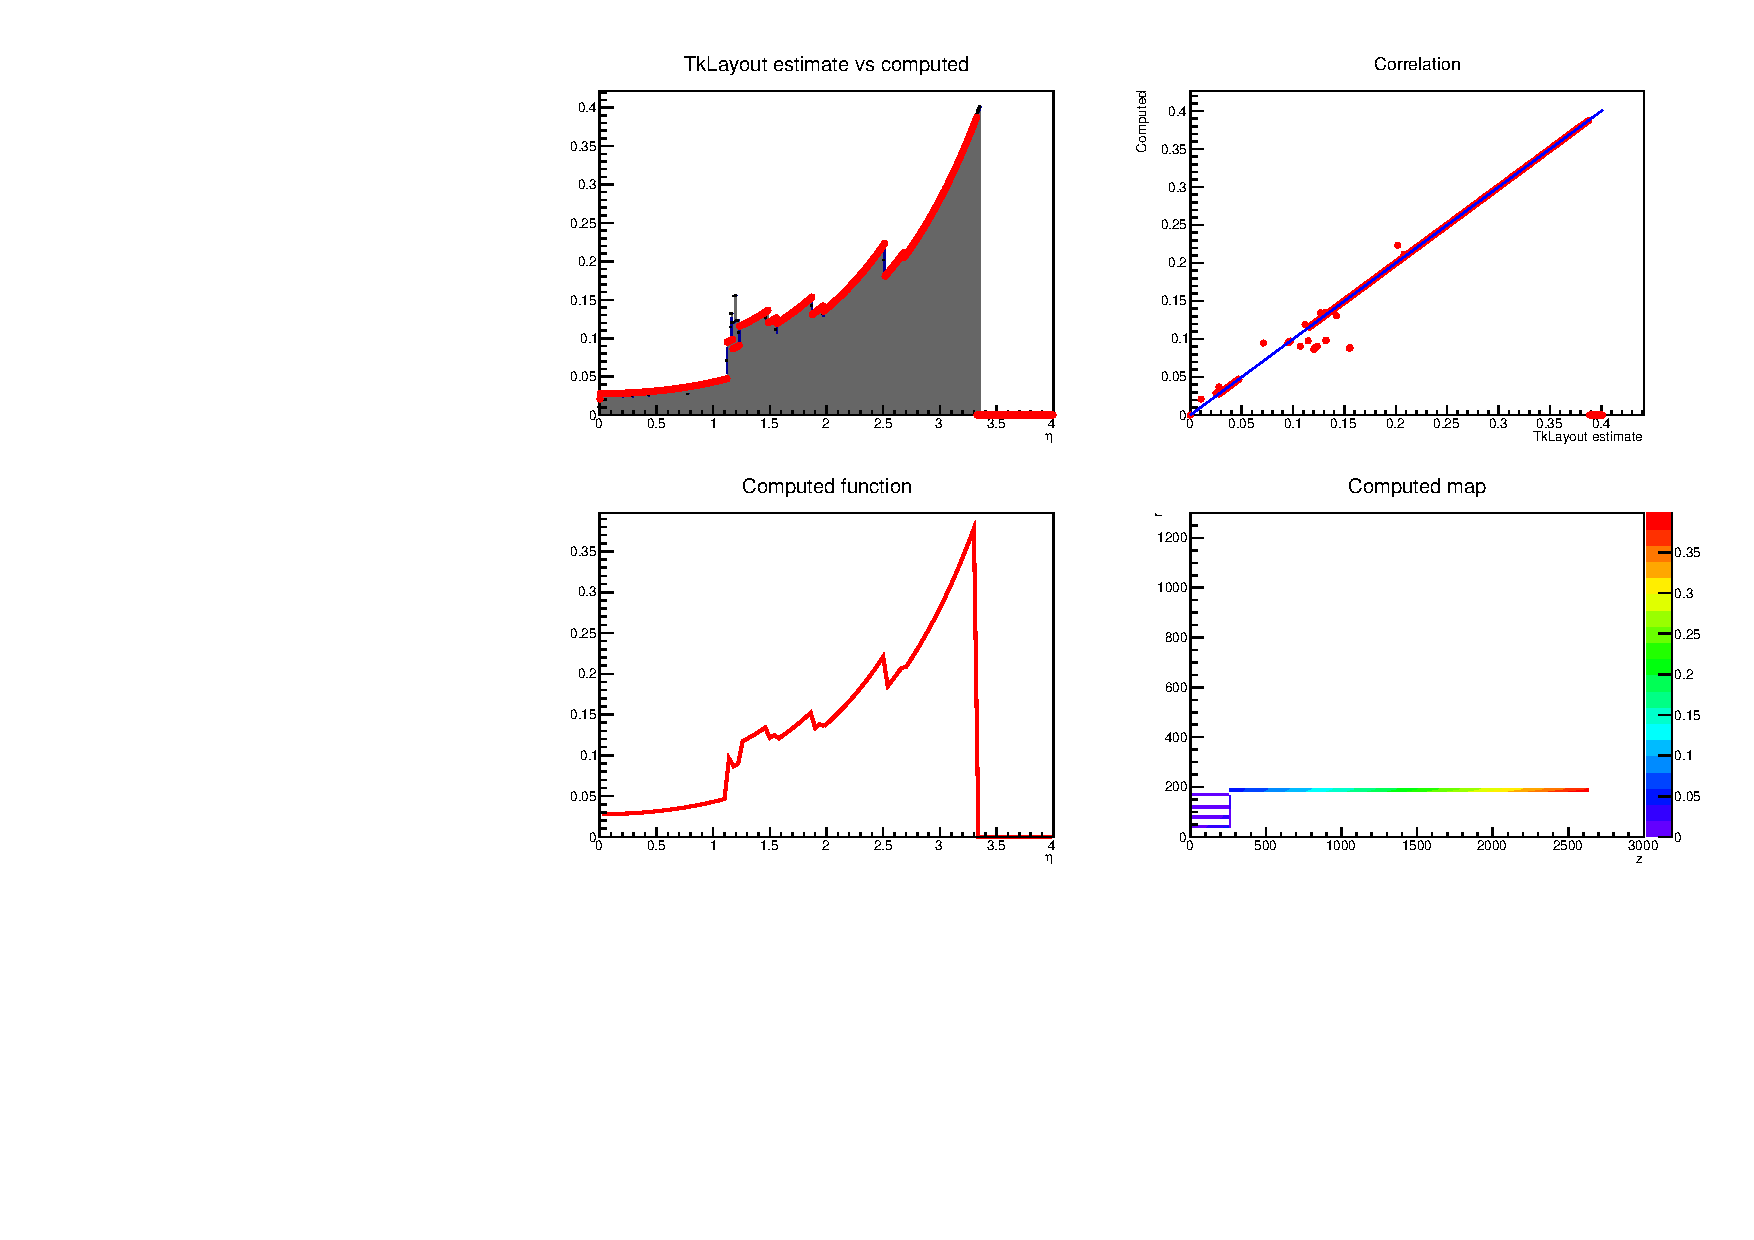
\includegraphics[width=9cm]{img/test3.pdf}
  \end{center}
\end{frame}

\begin{frame}
  \begin{block}{Test3bis}
    \alert{$0.1 mm$} of \emph{Cu}  in the rods of first layer of the pixel barrel, not exiting
    \begin{itemize}
    \item \alert{$L=0.1$} for all elements
    \end{itemize}
  \end{block}
  \begin{center}
    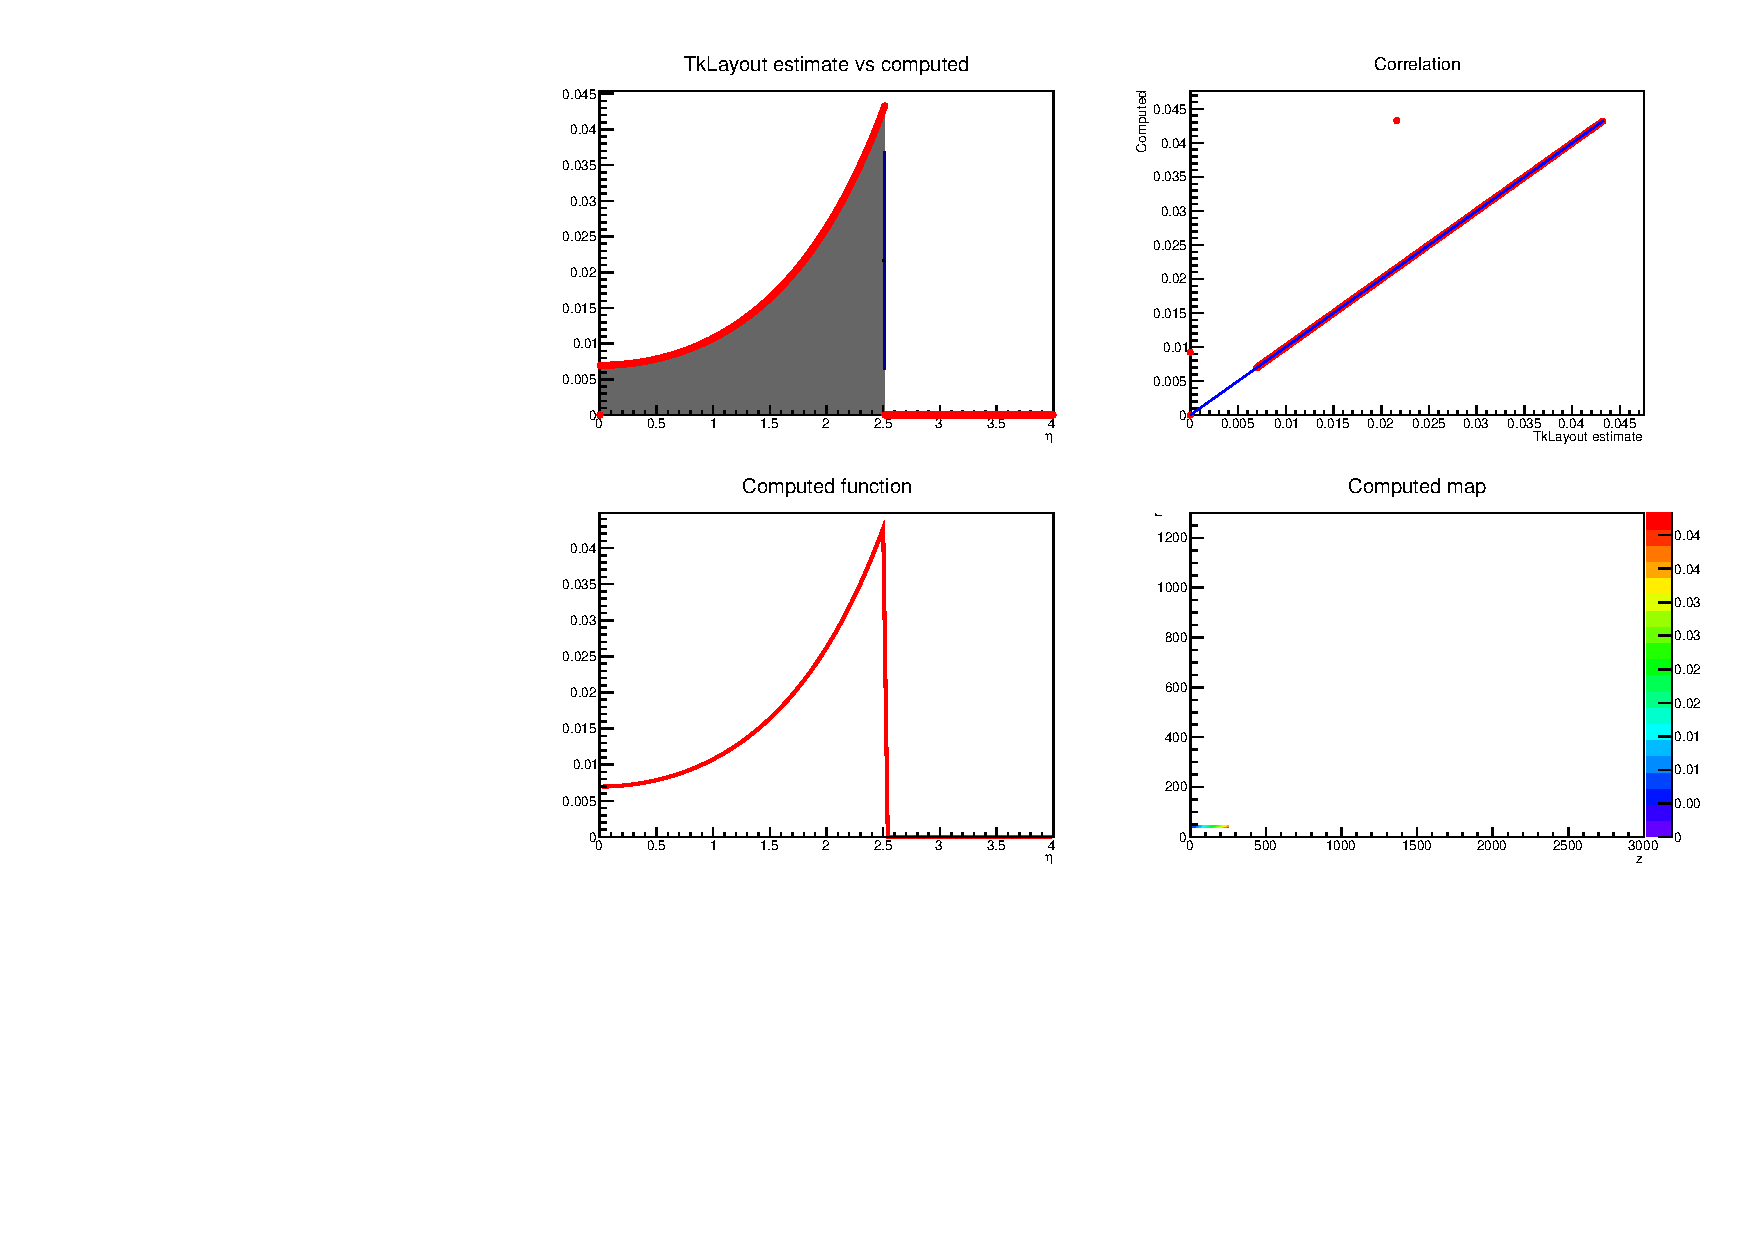
\includegraphics[width=9cm]{img/test3bis.pdf}
  \end{center}
\end{frame}

\begin{frame}
  \begin{block}{Test3ter}
    \alert{$0.1 mm$} of \emph{Cu}  in the rods of all the layers of the pixel barrel, not exiting
    \begin{itemize}
    \item \alert{$L=0.1$} for layers
    \end{itemize}
  \end{block}
  \begin{center}
    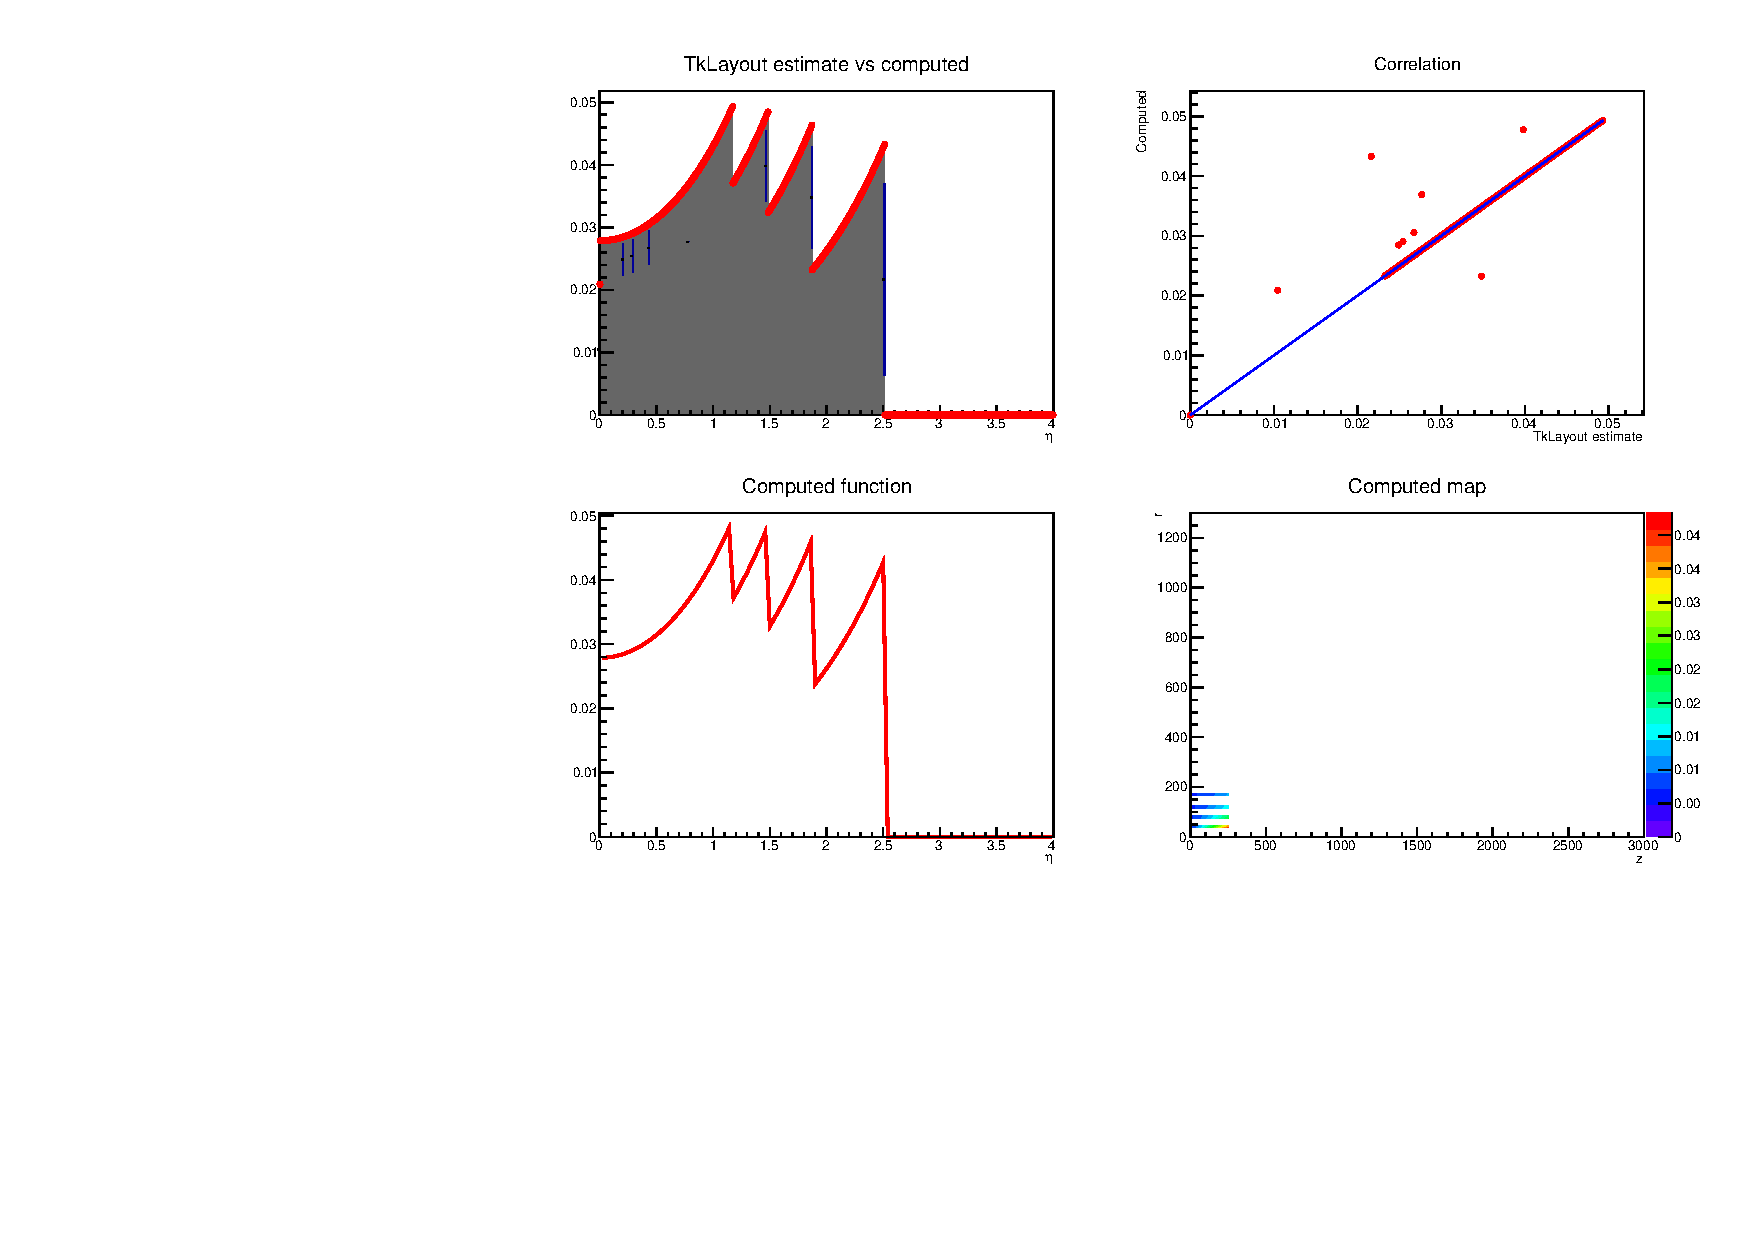
\includegraphics[width=9cm]{img/test3ter.pdf}
  \end{center}
\end{frame}

\begin{frame}
  \begin{block}{Test3quater}
    \alert{$0.1 mm$} of \emph{Cu}  in the rods of first layer of the pixel barrel, exiting
    \begin{itemize}
    \item \alert{$L=0.1$} for all elements
    \end{itemize}
  \end{block}
  \begin{center}
    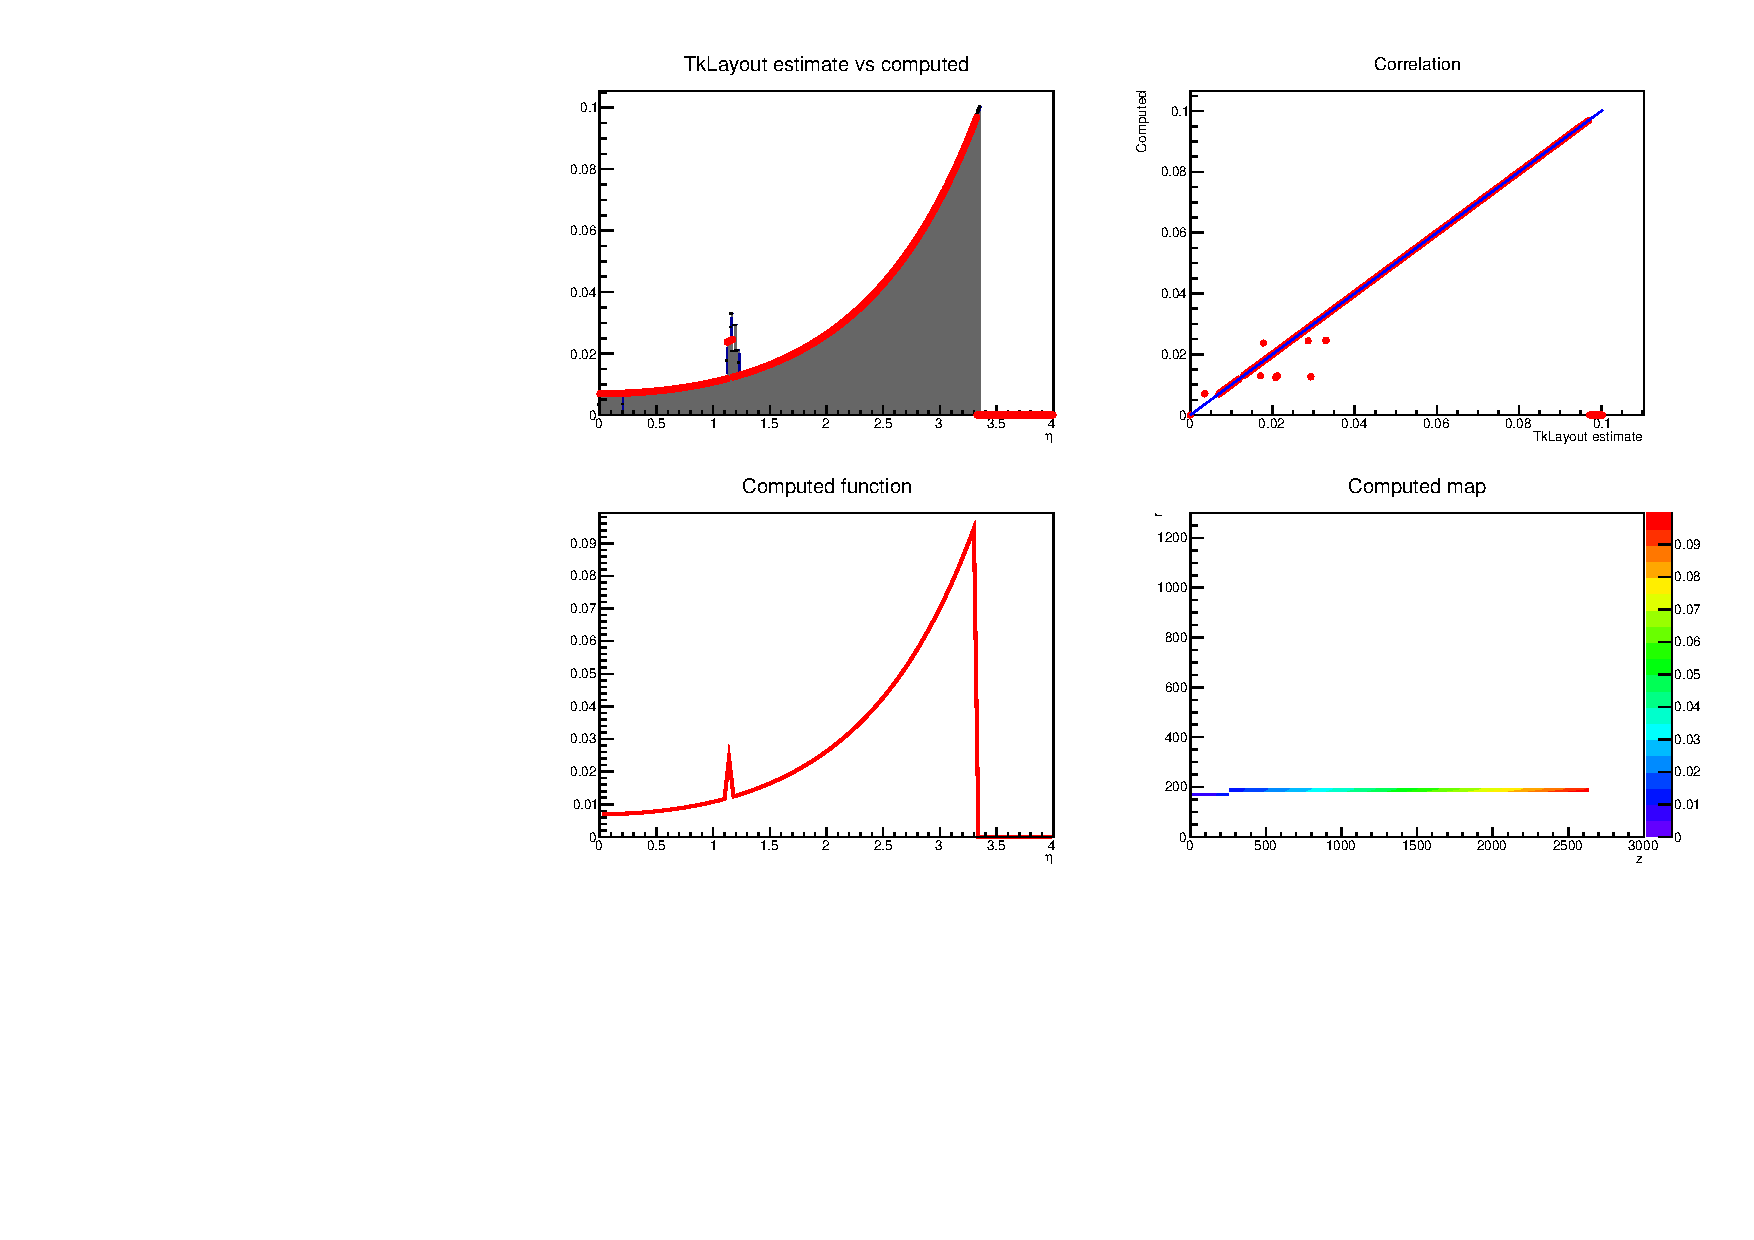
\includegraphics[width=9cm]{img/test3quater.pdf}
  \end{center}
\end{frame}

\begin{frame}
  \begin{block}{Test4}
    \alert{$100 g/m$} of \emph{Cu} exiting from modules of the first layer of the pixel barrel
    \begin{itemize}
    \item \alert{$L=(rods*100) + L_{previousCylinder}$} for cylinders
    \end{itemize}
  \end{block}
  \begin{center}
    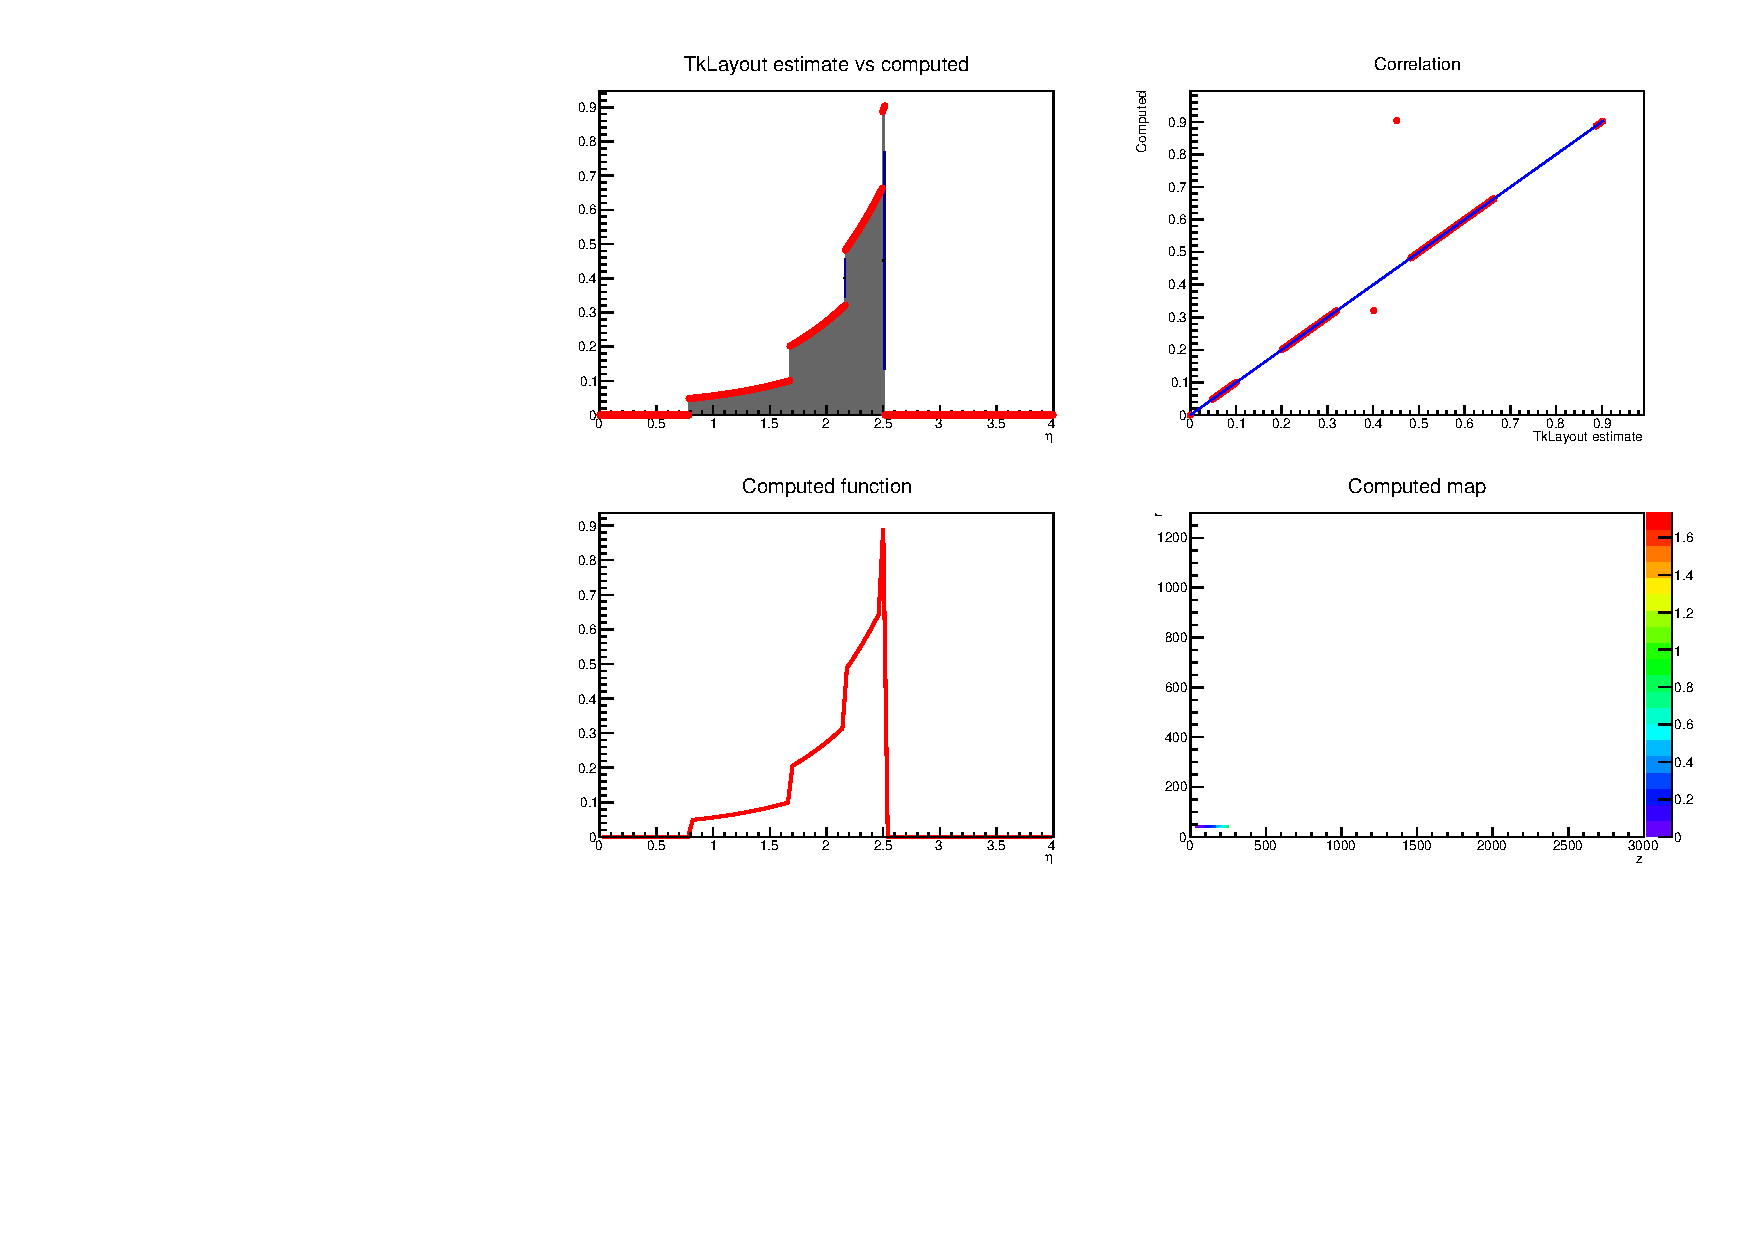
\includegraphics[width=9cm]{img/test4.pdf}
  \end{center}
\end{frame}

\begin{frame}
  \begin{block}{Test5}
    \alert{$100 g/m$} of \emph{Cu} exiting from modules and \alert{$150 g/m$} in the rods
    \begin{itemize}
    \item \alert{$L=(rods*100) + L_{previousCylinder}$} for cylinders
    \item \alert{$L=(rods*150)$} in layer
    \end{itemize}
  \end{block}
  \begin{center}
    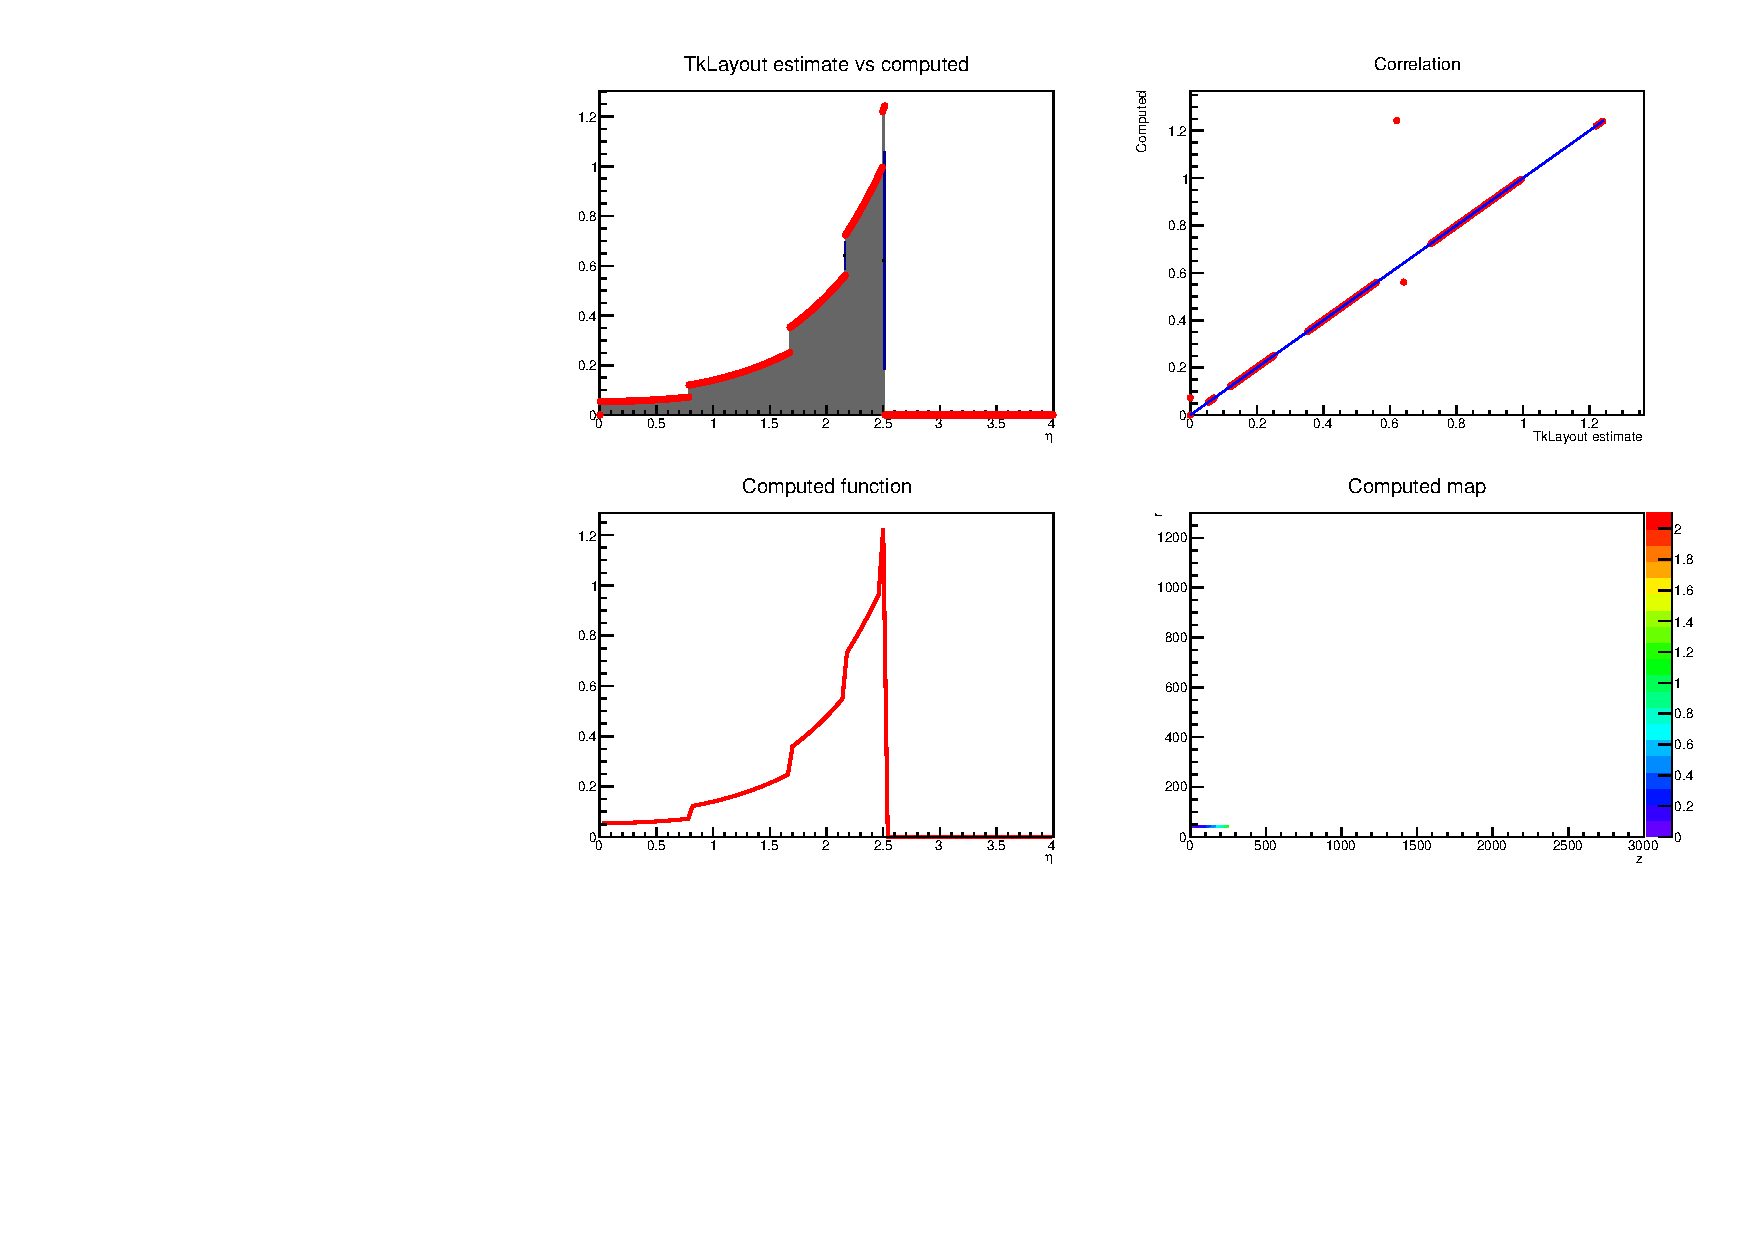
\includegraphics[width=9cm]{img/test5.pdf}
  \end{center}
\end{frame}

\begin{frame}
  \begin{block}{Test6}
    \alert{$100 g/m$} of \emph{Cu} in the first disk of pixel endcap
    \begin{itemize}
    \item \alert{$24$} modules on first ring of disk
    \item \alert{$L=(24*100)$} in every element
    \end{itemize}
  \end{block}
  \begin{center}
    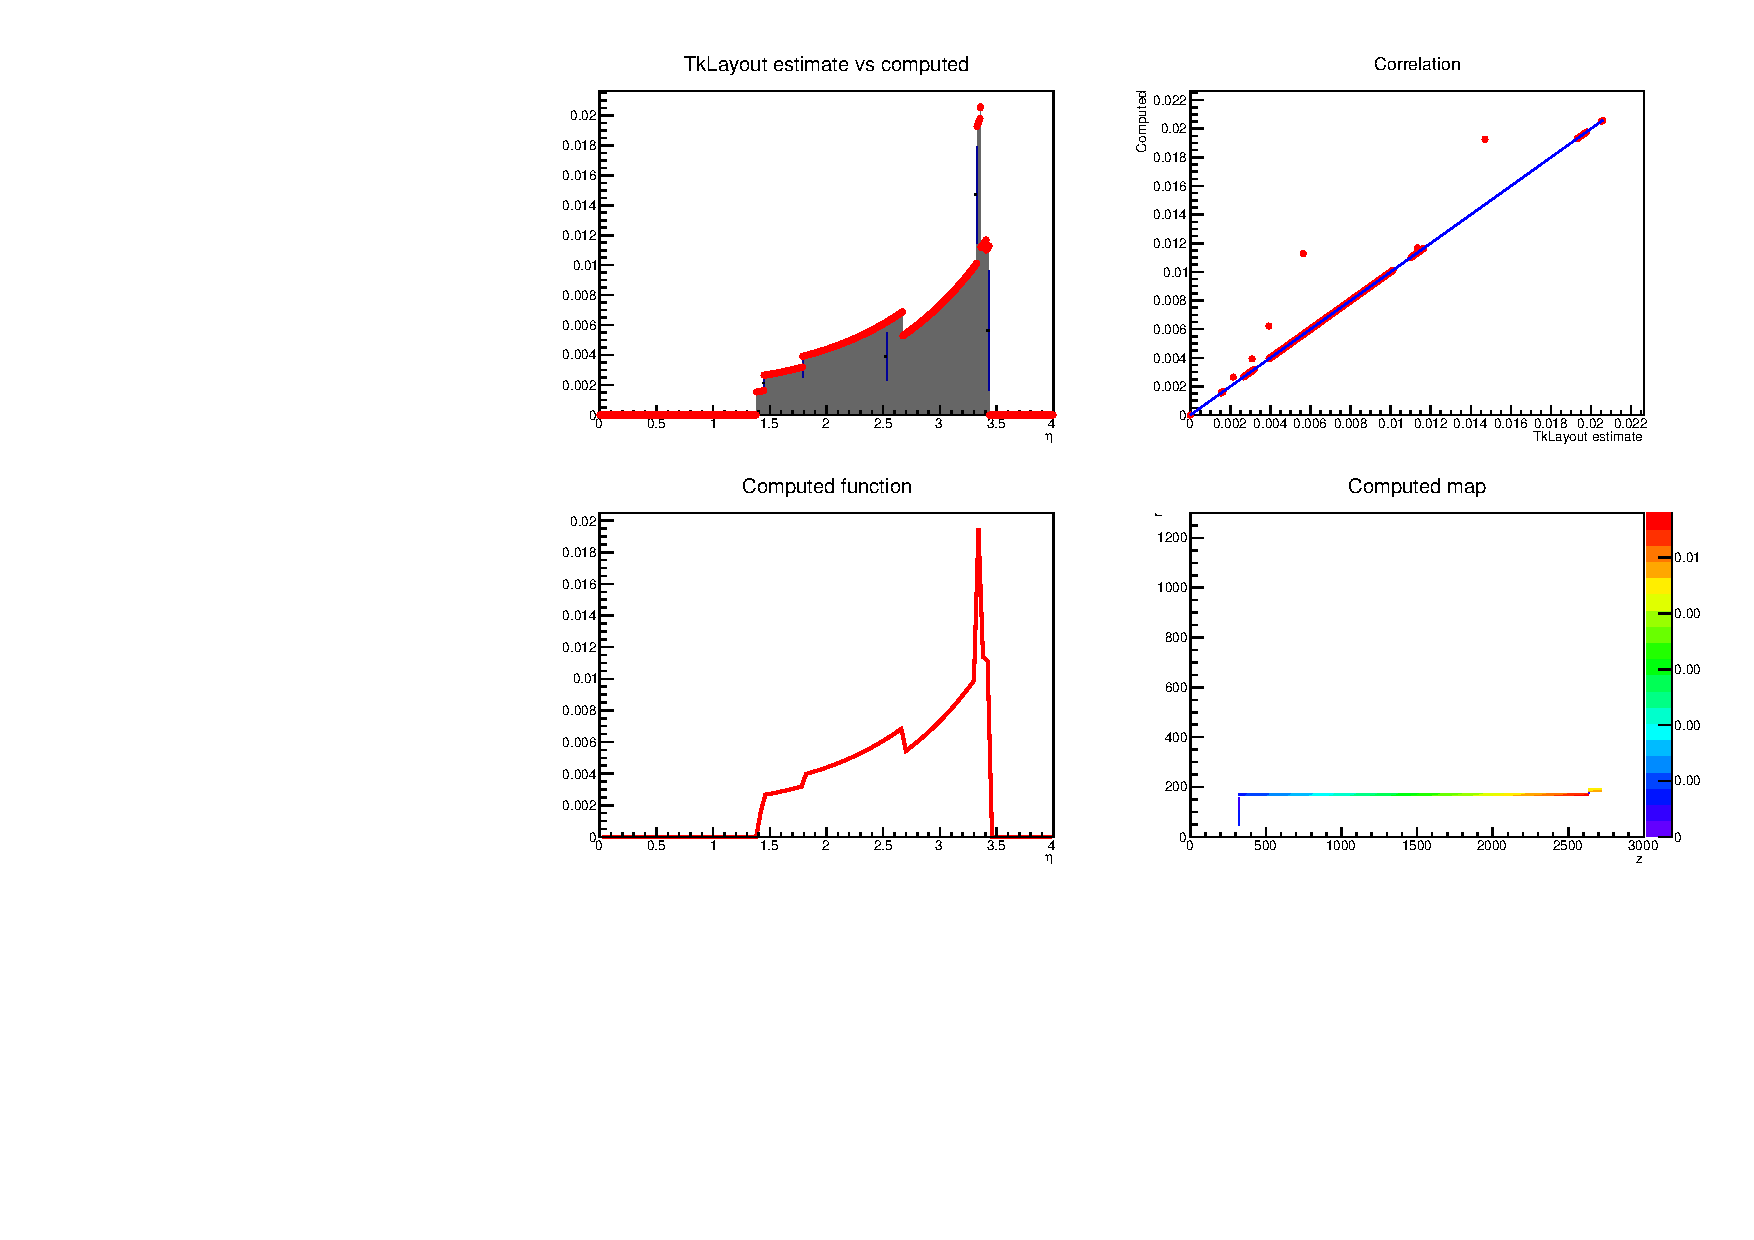
\includegraphics[width=9cm]{img/test6.pdf}
  \end{center}
\end{frame}

\begin{frame}
  \begin{block}{Test6bis}
    \alert{$100 g/m$} of \emph{Cu} exiting from the first disk modules of pixel endcap
    \begin{itemize}
    \item \alert{$24$} modules on first ring of disk, \alert{$36$} on second
    \item \alert{$L=(24*100)$} in service disk, \alert{$L=(60*100)$} in others
    \end{itemize}
  \end{block}
  \begin{center}
    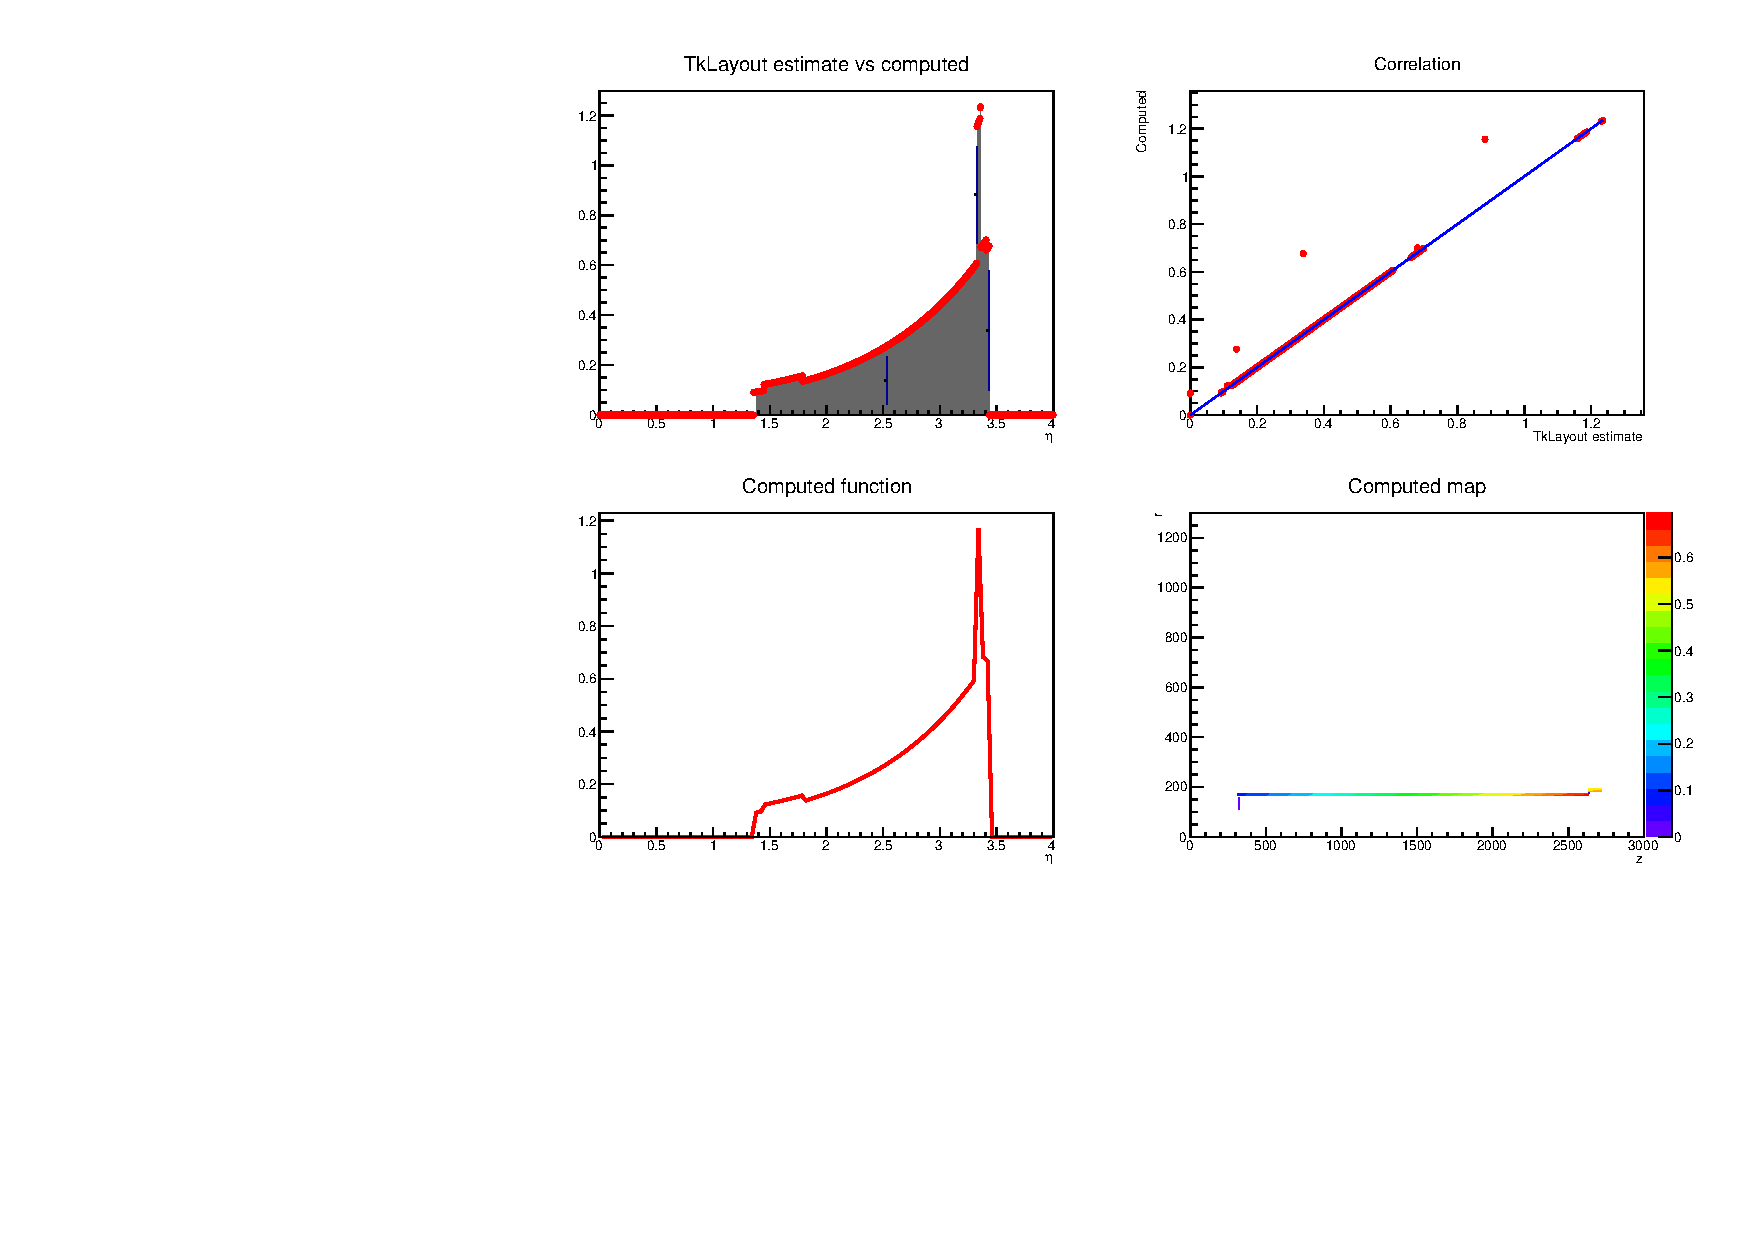
\includegraphics[width=9cm]{img/test6bis.pdf}
  \end{center}
\end{frame}

\begin{frame}
  \begin{block}{Test7}
    \alert{$100 g/m$} of \emph{Cu} in the fourth layer and conversion \alert{$1g/m\to 0.1g$ locally}
    \begin{itemize}
    \item \alert{$L=(rods*100)$} in layer
    \item \alert{$L=(rods*100*0.1)$} in flange
    \end{itemize}
  \end{block}
  \begin{center}
    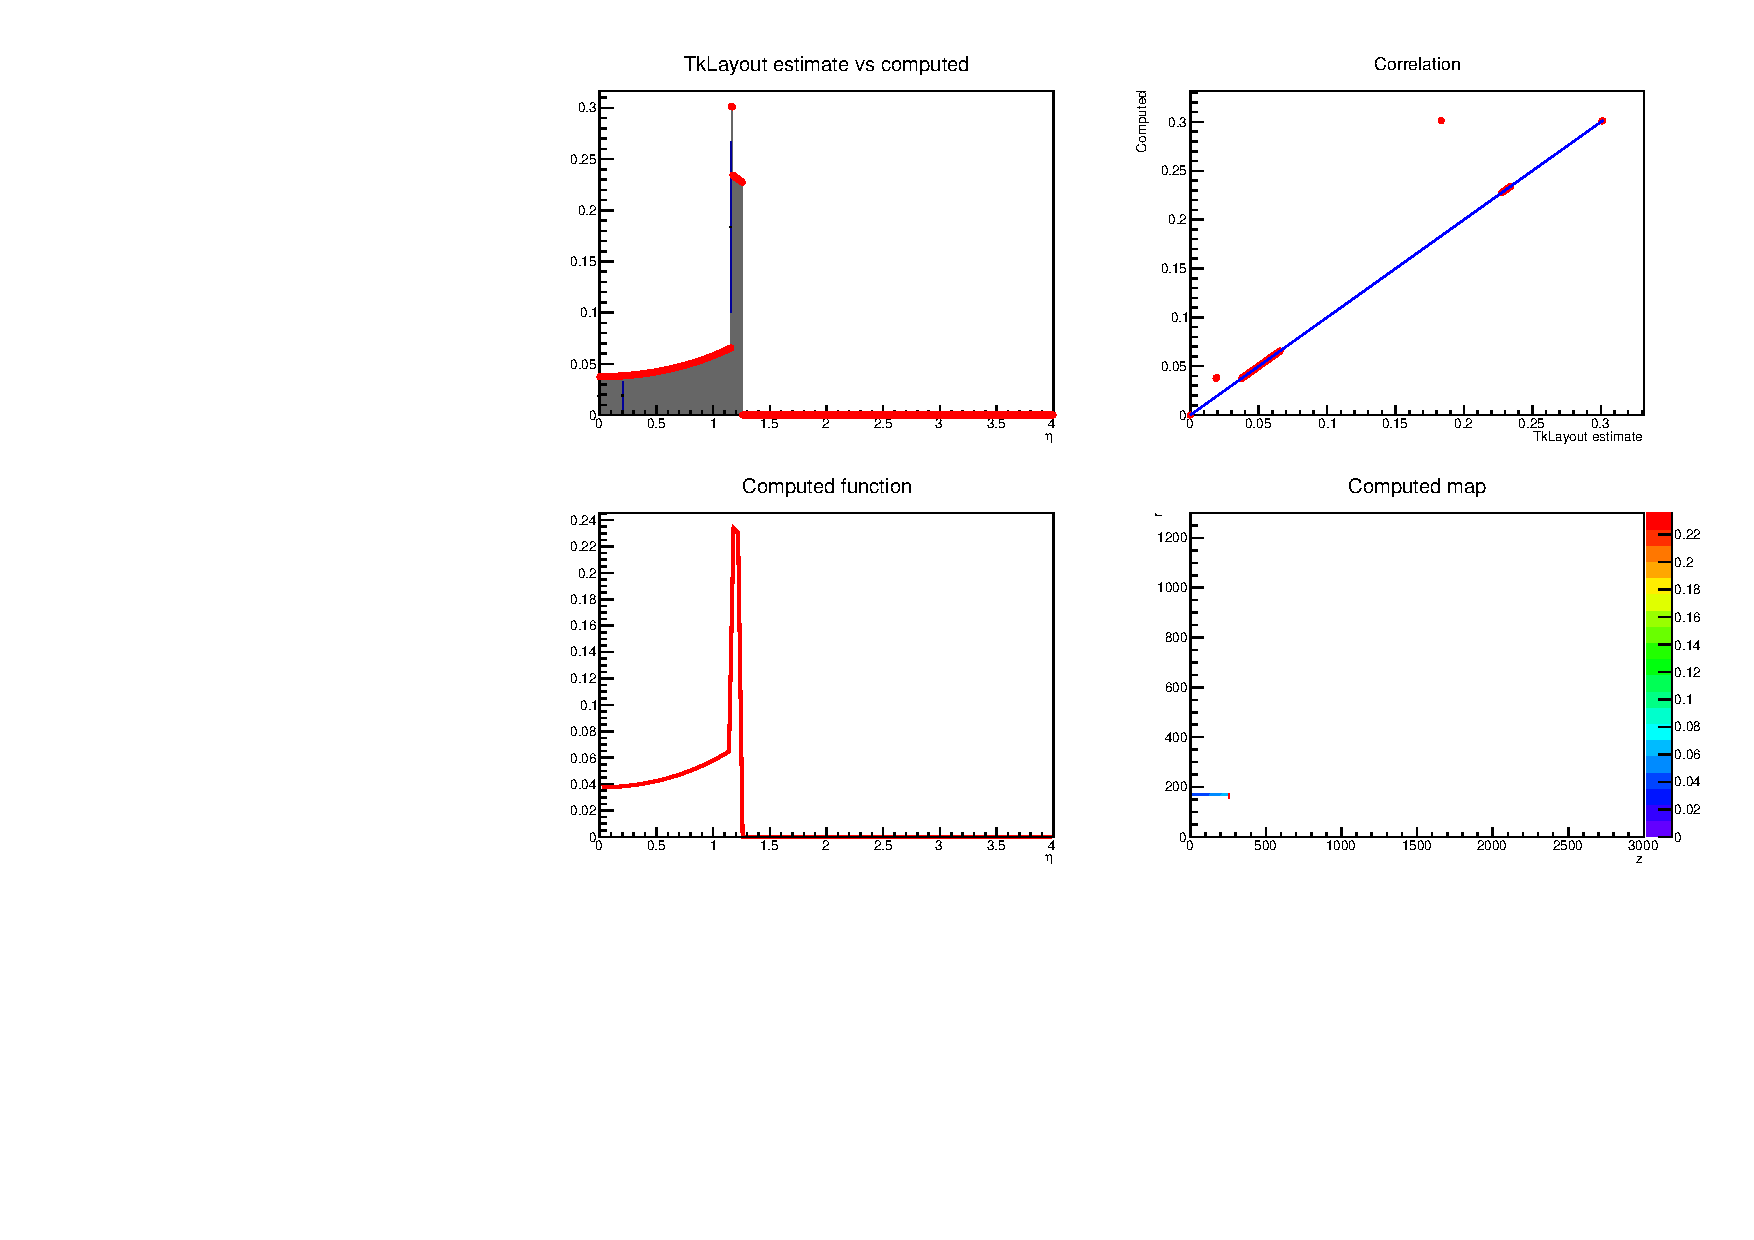
\includegraphics[width=9cm]{img/test7.pdf}
  \end{center}
\end{frame}

\begin{frame}
  \begin{block}{Test8}
    \alert{$100 g/m$} of \emph{Cu} in the fourth layer and conversion \alert{$1g/m\to 1.5g/m$ exiting}
    \begin{itemize}
    \item \alert{$L=(rods*100)$} in layer
    \item \alert{$L=(rods*150)$} in second cylinder
    \end{itemize}
  \end{block}
  \begin{center}
    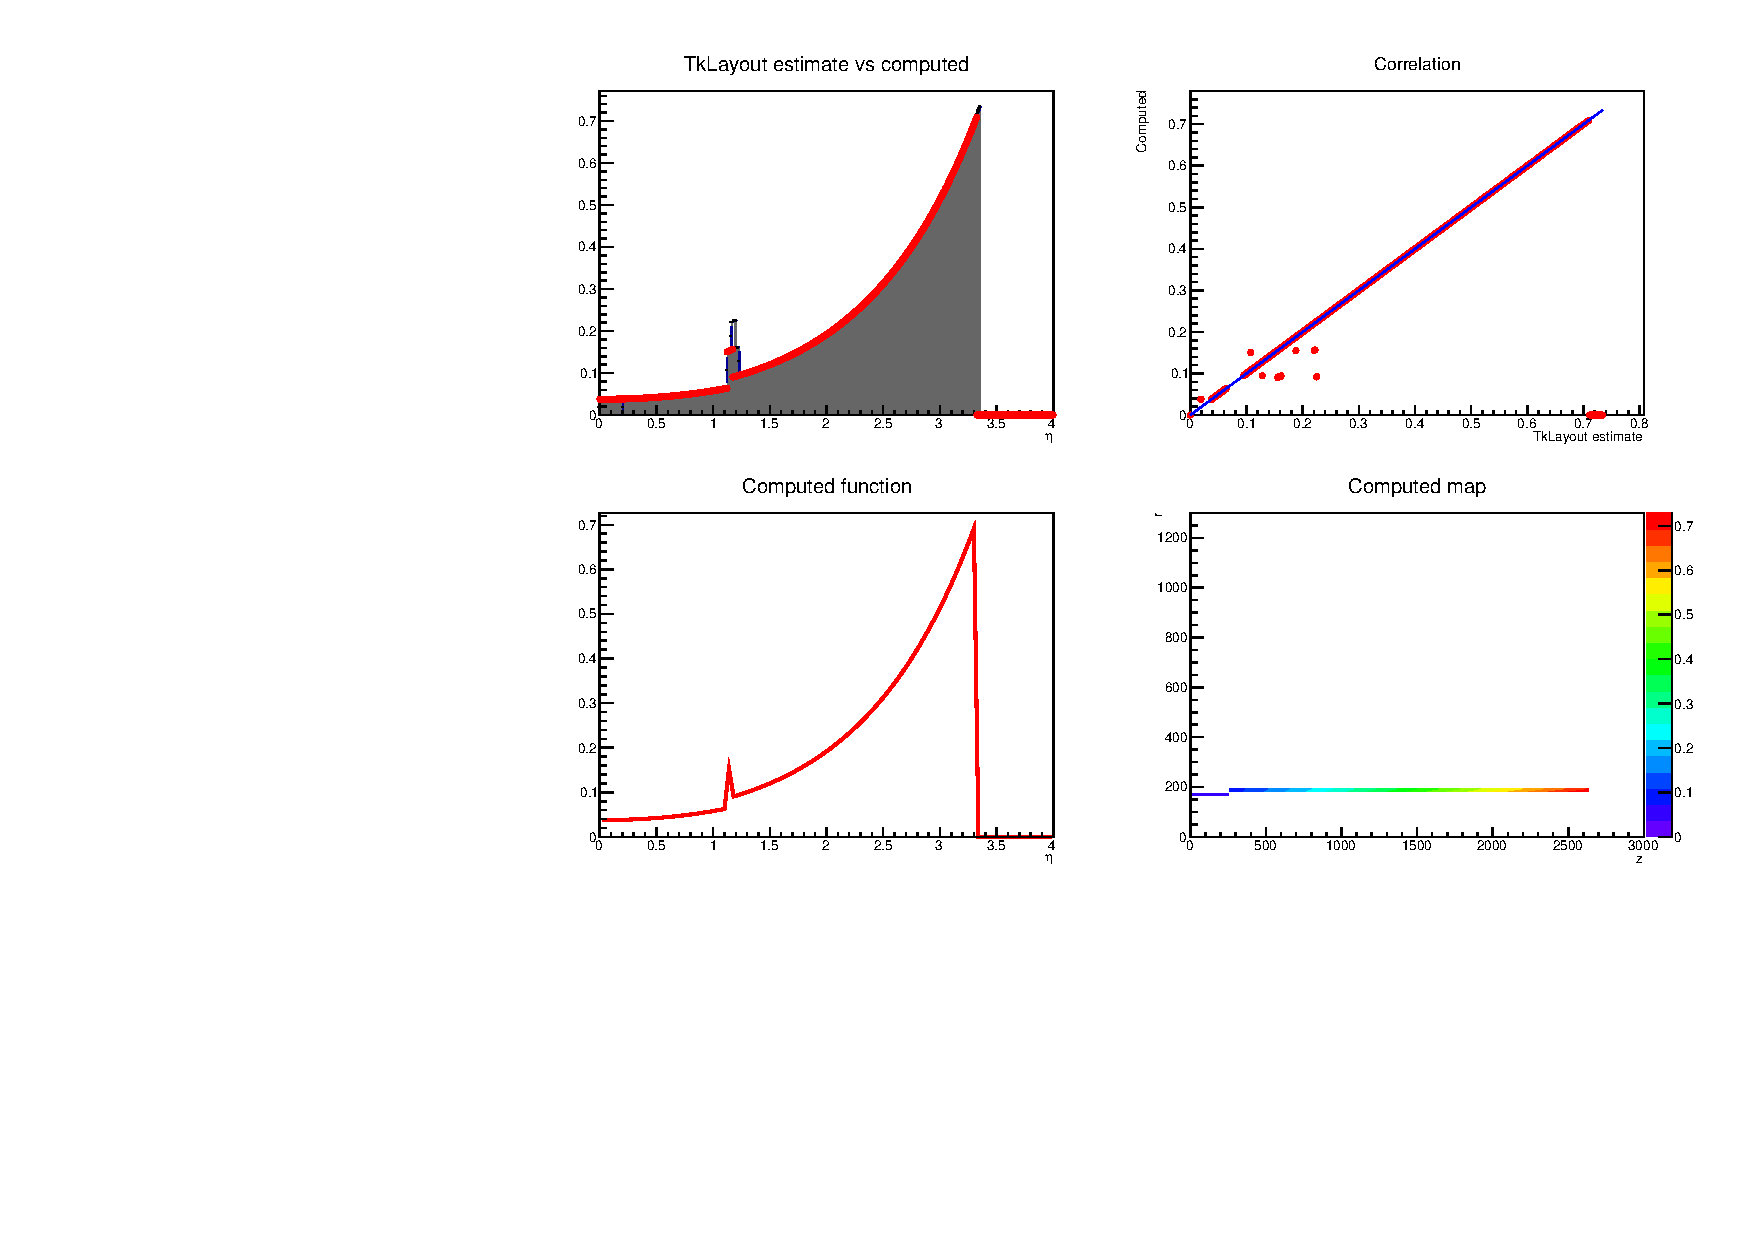
\includegraphics[width=9cm]{img/test8.pdf}
  \end{center}
\end{frame}

\begin{frame}
  \begin{block}{Test9}
    \alert{$100 g/m$} of \emph{Cu} and \alert{$150 g/m$} of \emph{Al} in the fourth layer and conversions
    \begin{itemize}
    \item \alert{$1g/m Cu\to 2g/m Cu$} exiting
    \item \alert{$0.1g/m Al\to 0.15g/m Al$} exiting
    \end{itemize}
  \end{block}
  \begin{center}
    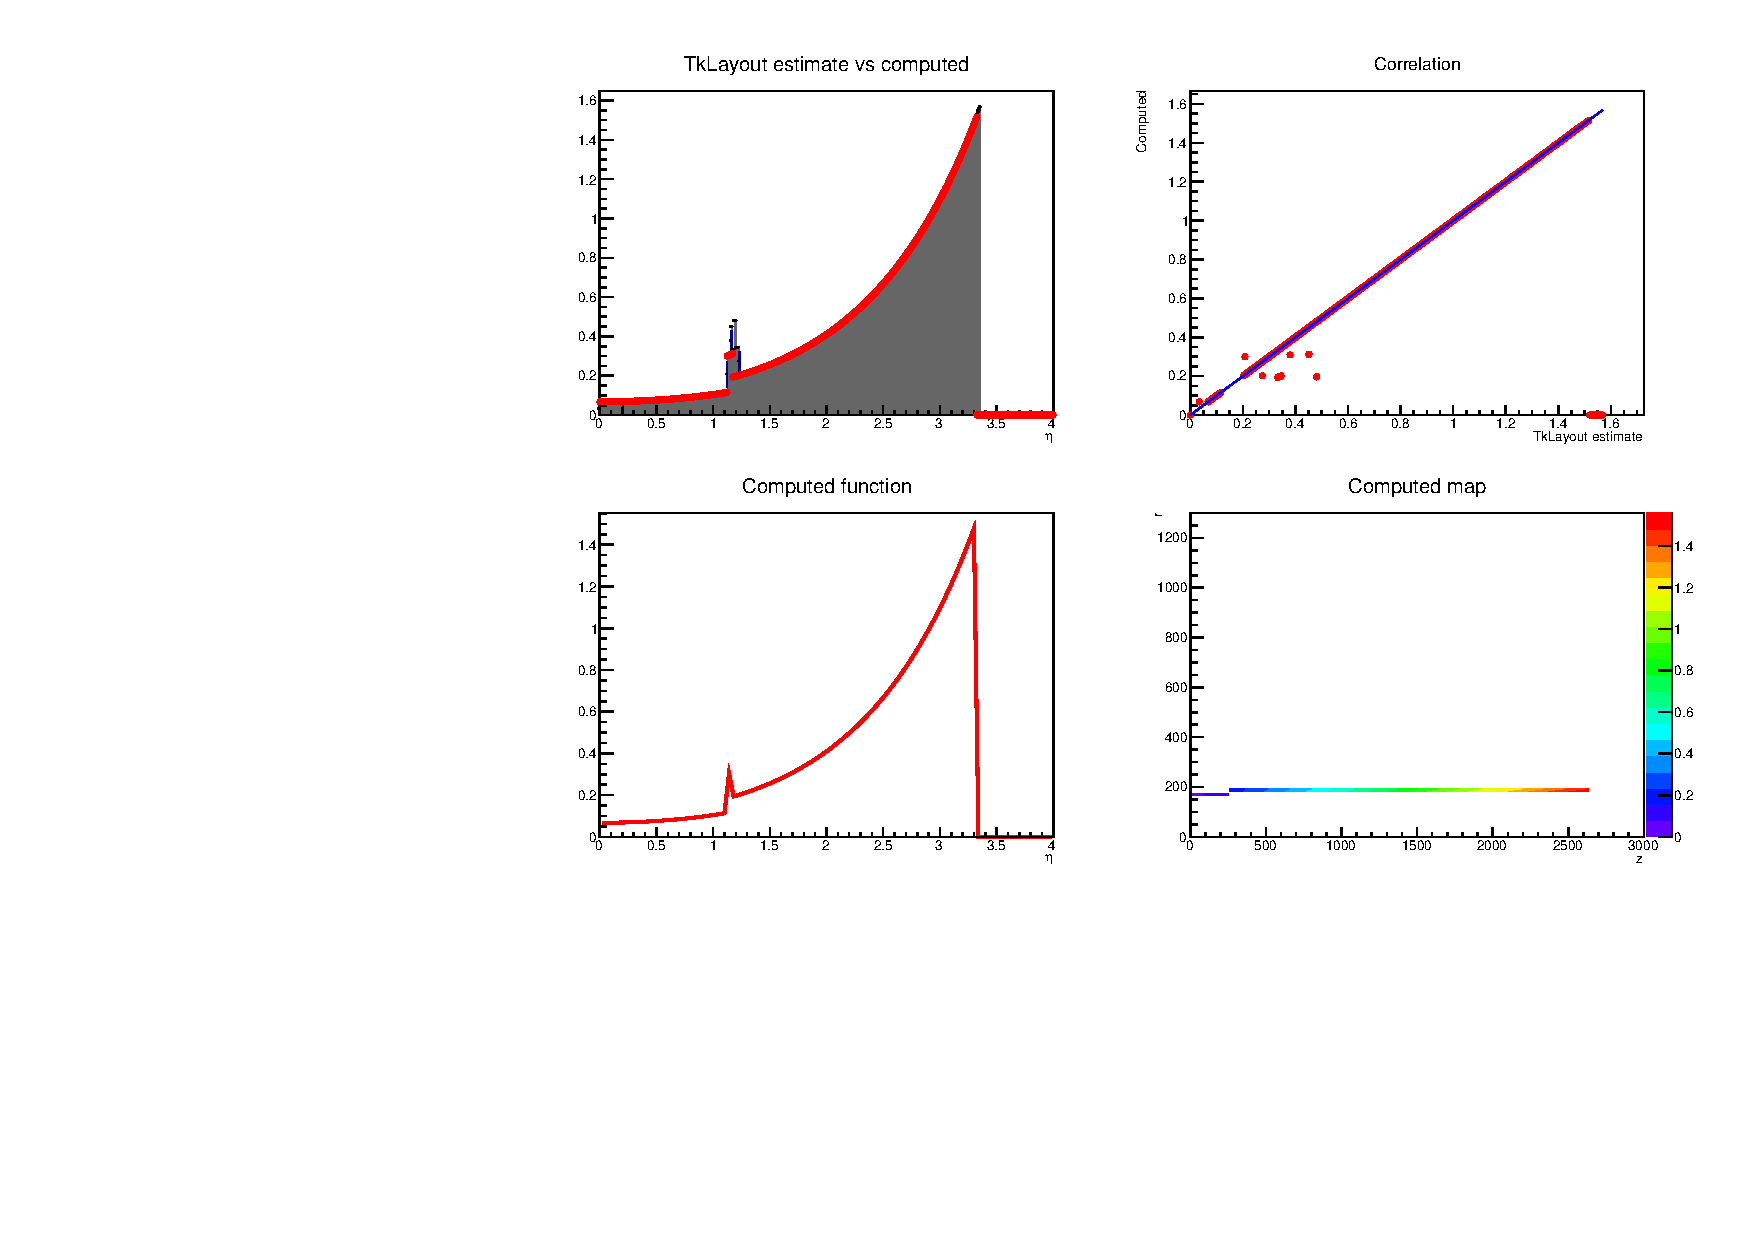
\includegraphics[width=9cm]{img/test9.pdf}
  \end{center}
\end{frame}

\begin{frame}
  \begin{block}{Test10}
    \alert{$100 g/m$} of \emph{Cu} in the fourth layer and conversions
    \begin{itemize}
    \item \alert{$1g/m\to 1g/m$} exiting in the flange
    \item \alert{$1g/m\to 0.1g$} local in the second level
    \end{itemize}
  \end{block}
  \begin{center}
    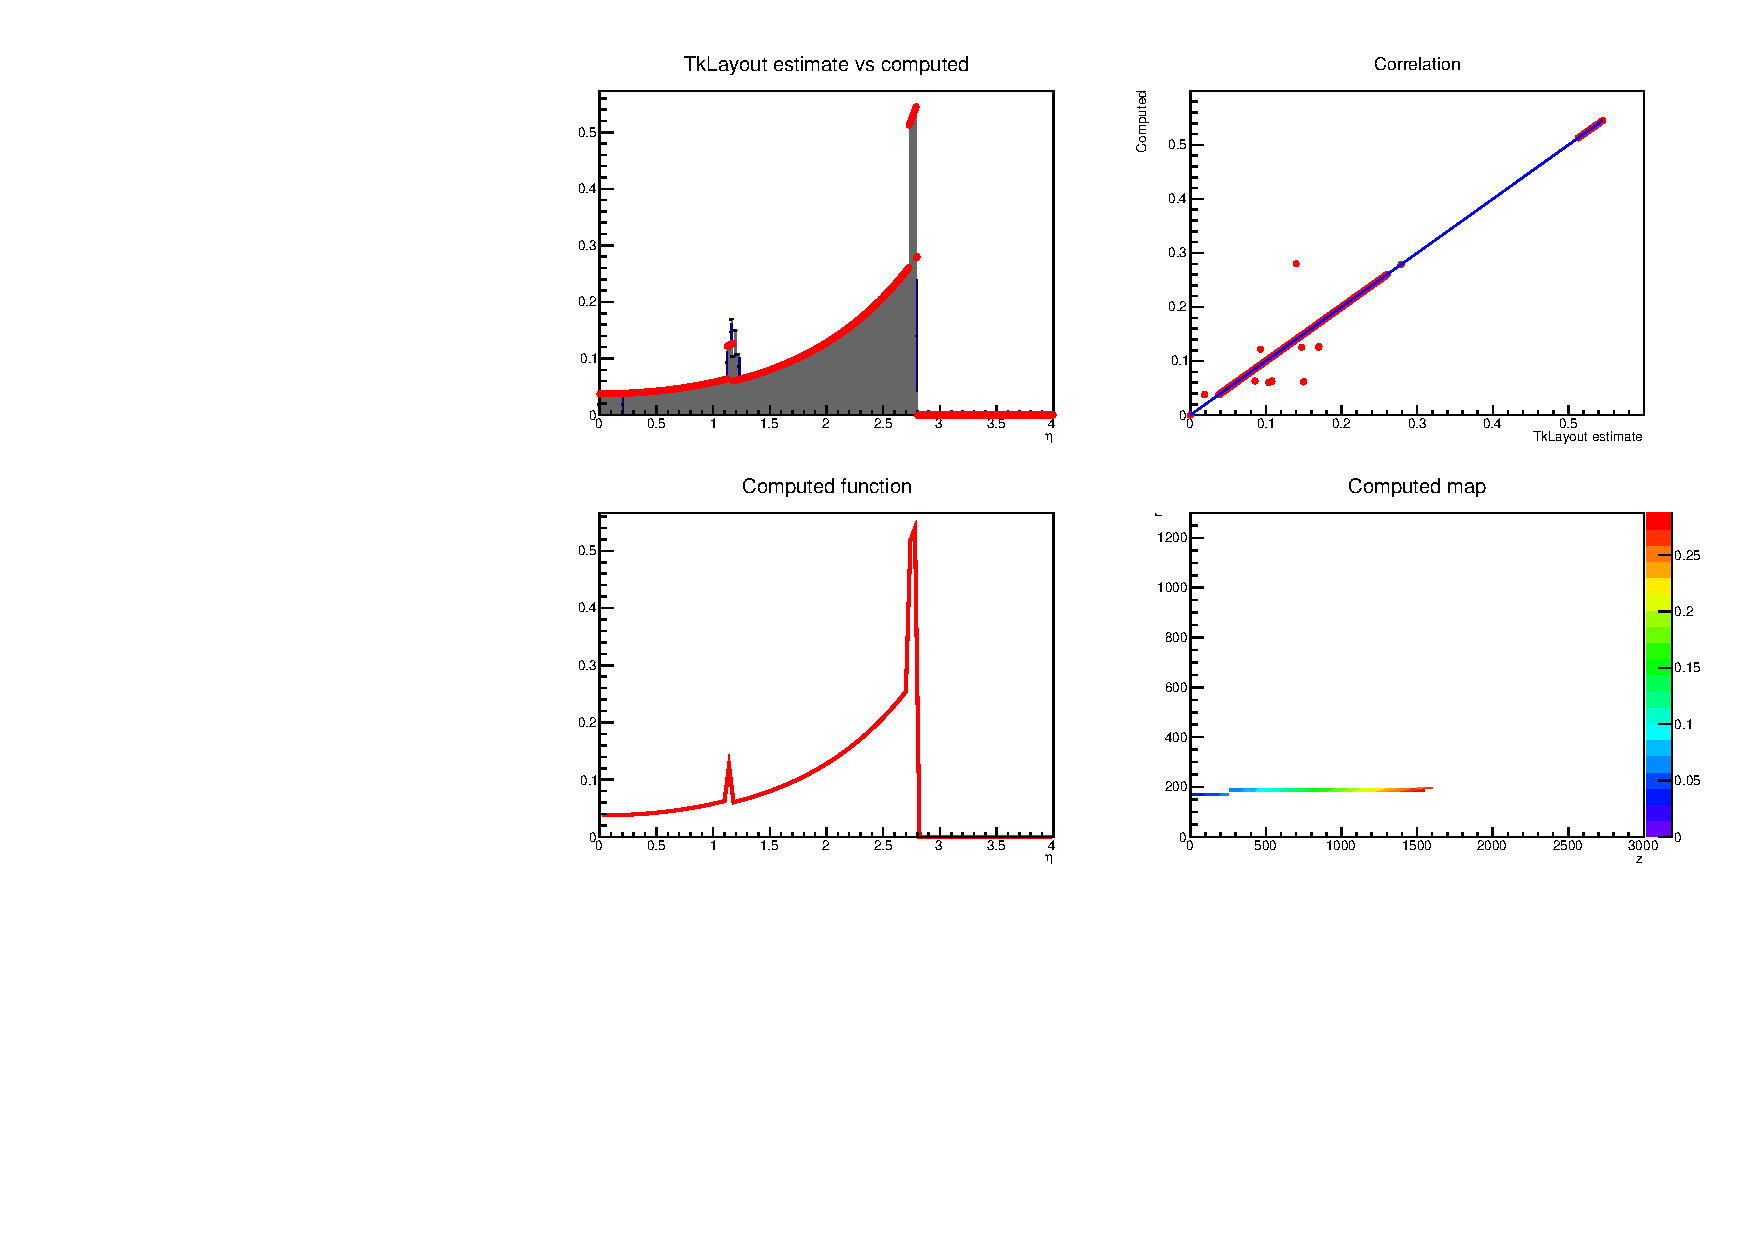
\includegraphics[width=9cm]{img/test10.pdf}
  \end{center}
\end{frame}

\begin{frame}
  \begin{block}{Test10bis}
    \alert{$100 g/m$} of \emph{Cu} in the fourth layer and conversions
    \begin{itemize}
    \item \alert{$1g/m\to 1g/m$} exiting in the flange
    \item \alert{$1g/m\to 0.1g$} local \alert{$+ 1.5g/m$} exiting in the second level
    \end{itemize}
  \end{block}
  \begin{center}
    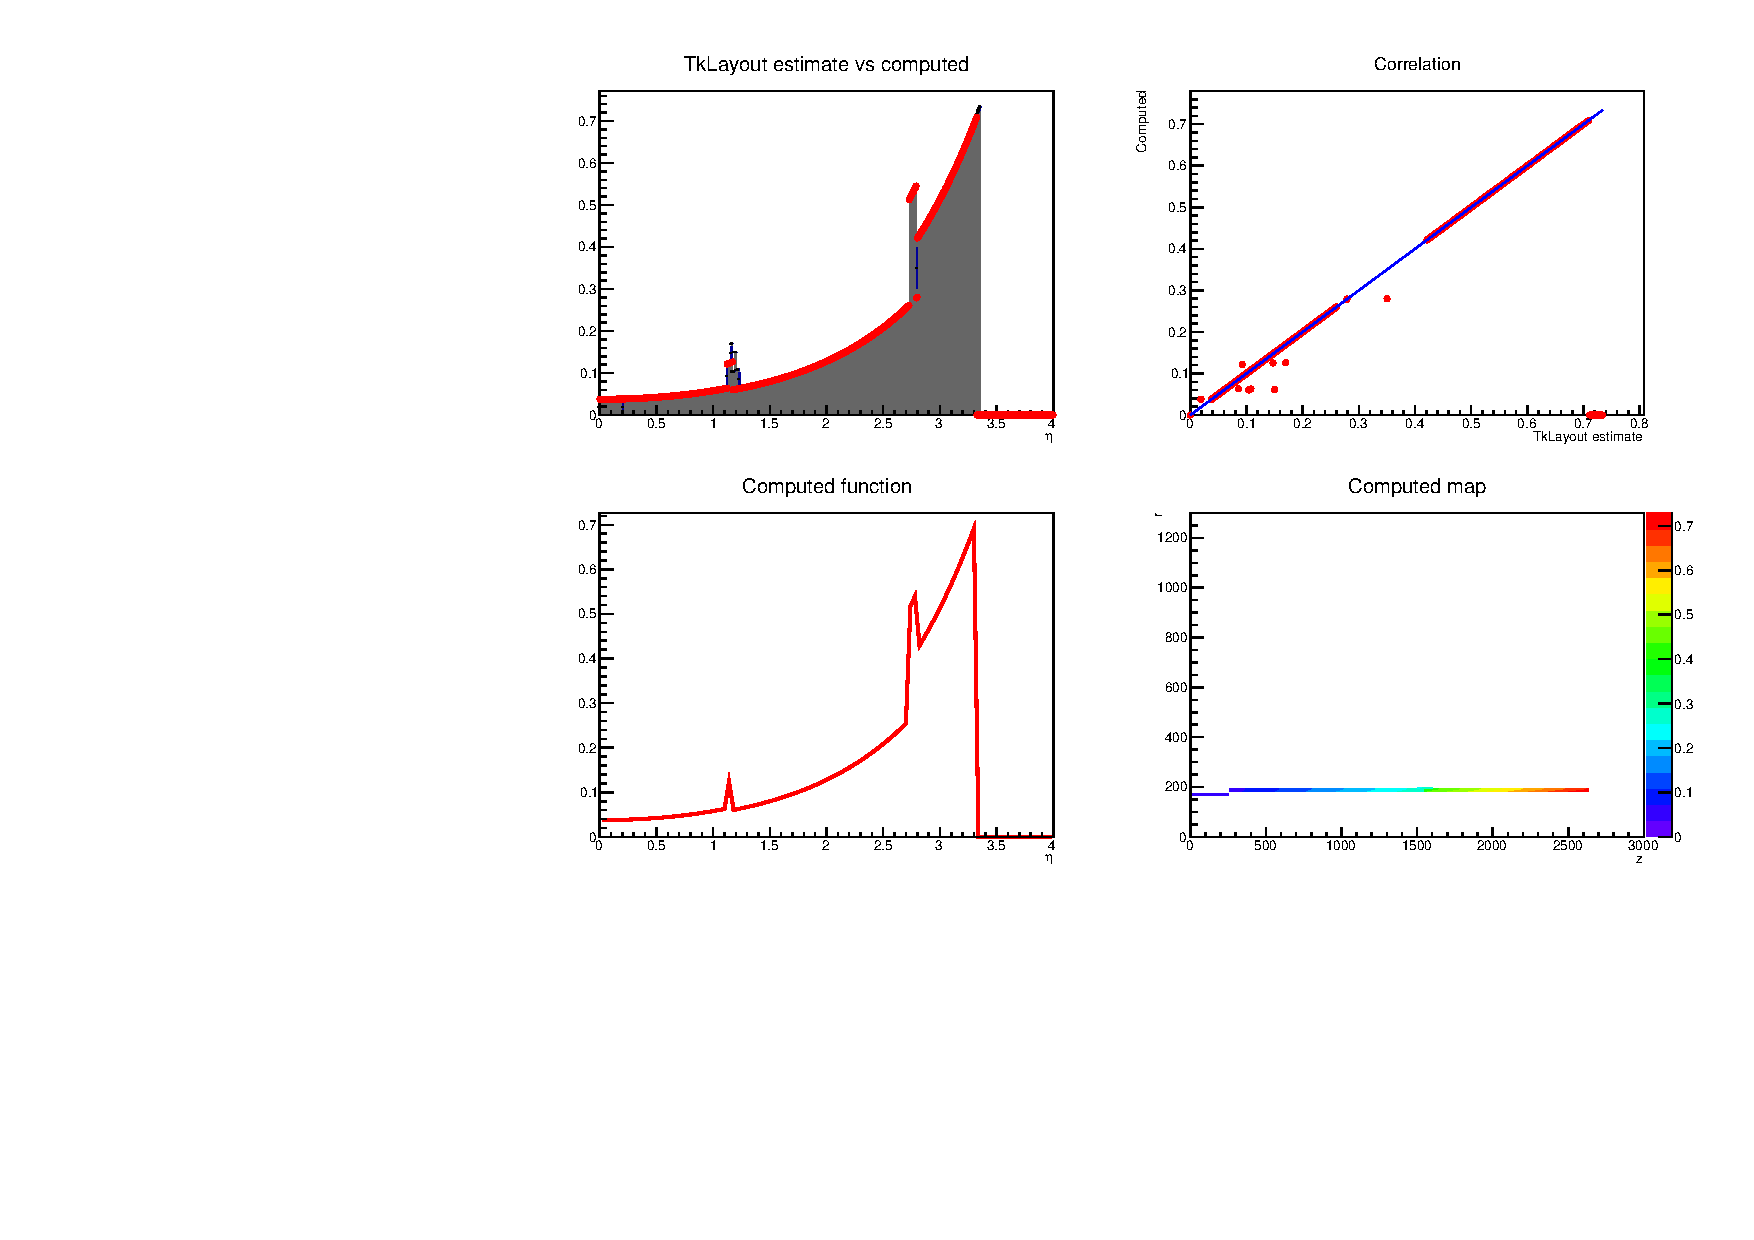
\includegraphics[width=9cm]{img/test10bis.pdf}
  \end{center}
\end{frame}

\begin{frame}
  \begin{block}{Test10ter}
    Same as test10bis plus \alert{$100 g/m$} of \emph{Cu}
    in the third layer with no destination for second level conversion
  \end{block}
  \begin{center}
    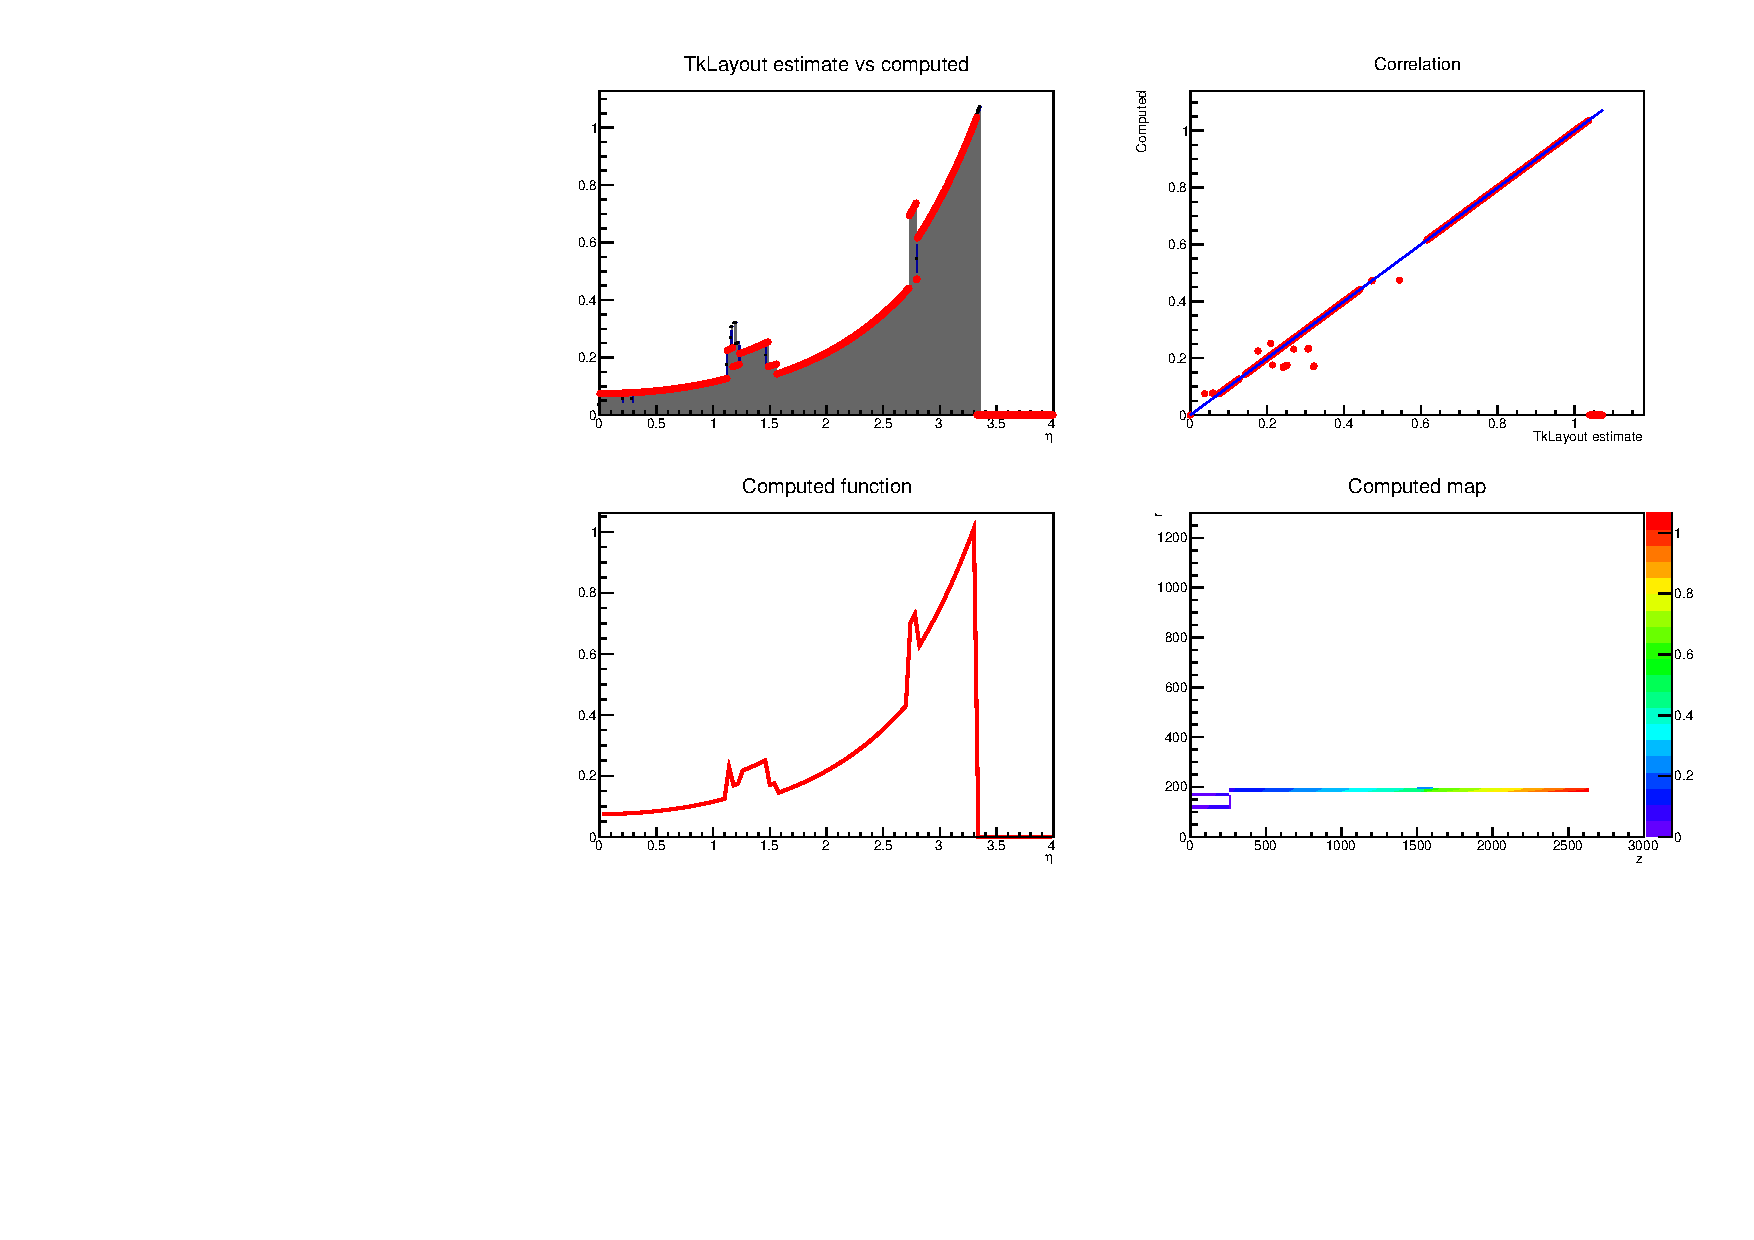
\includegraphics[width=9cm]{img/test10ter.pdf}
  \end{center}
\end{frame}

\begin{frame}
  \begin{block}{Test11}
    \alert{$100 g/m$} of \emph{Cu} exiting from modules of first layer with
    \begin{itemize}
    \item \alert{scaling} with reference \alert{strip numbers} halved
    \end{itemize}
  \end{block}
  \begin{center}
    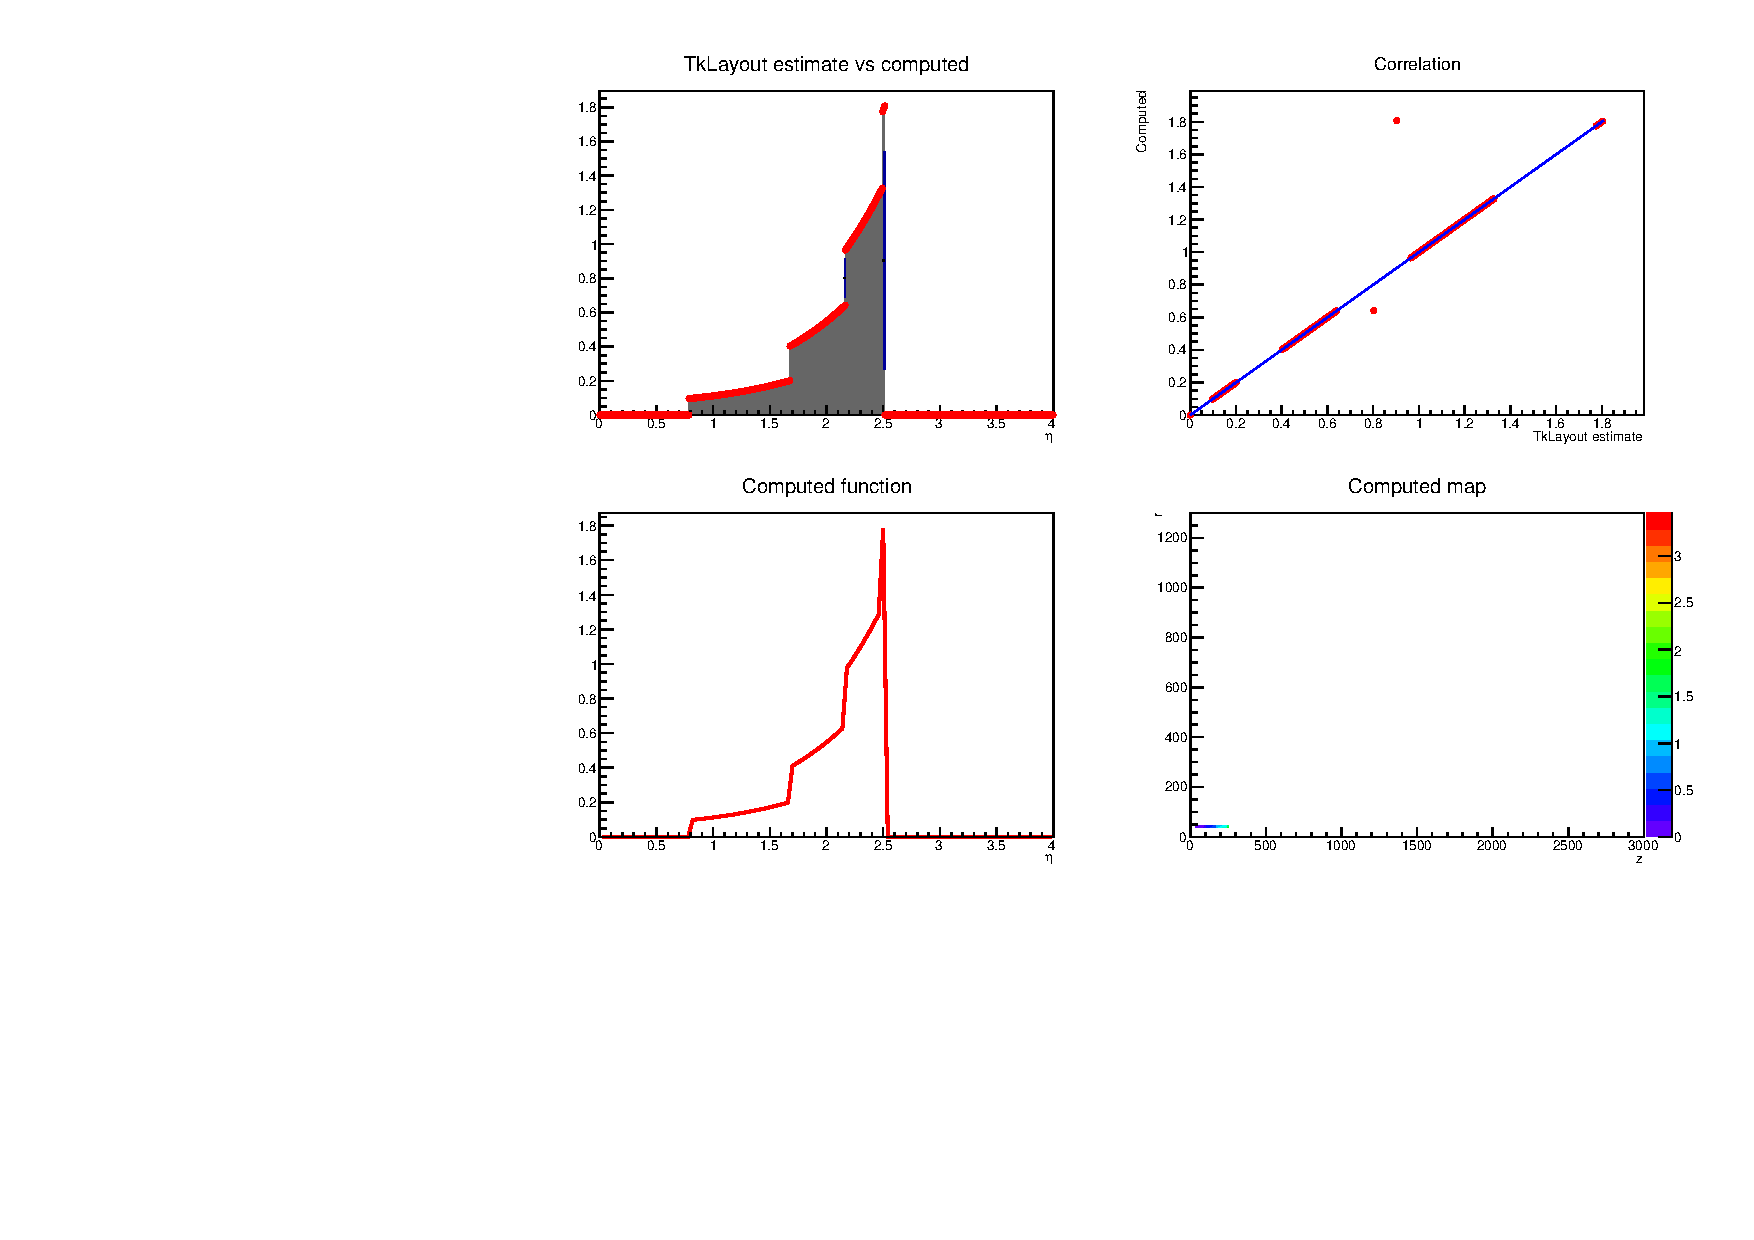
\includegraphics[width=9cm]{img/test11.pdf}
  \end{center}
\end{frame}

\begin{frame}
  \begin{block}{Test11bis}
    \alert{$100 g/m$} of \emph{Cu} exiting from modules of first layer with
    \begin{itemize}
    \item \alert{scaling} with reference \alert{segment numbers} halved
    \end{itemize}
  \end{block}
  \begin{center}
    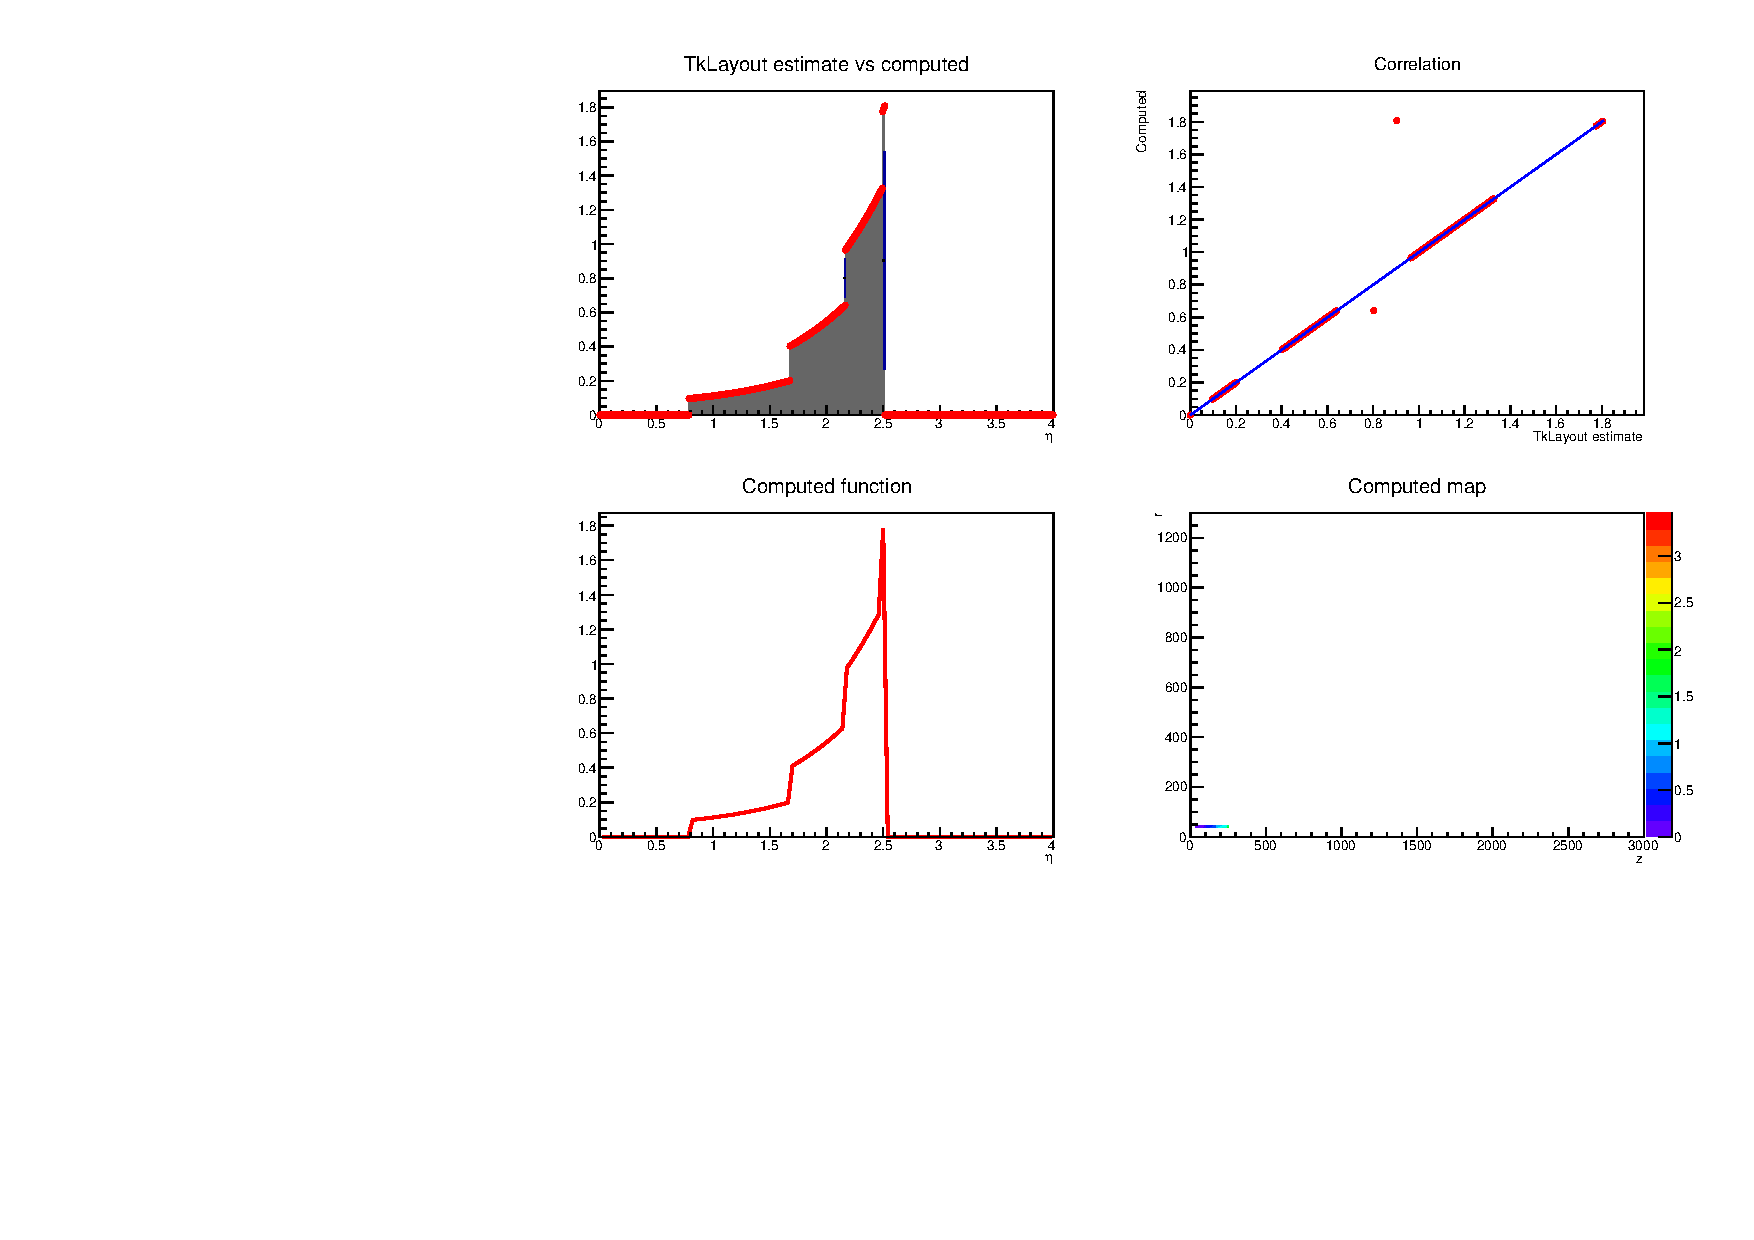
\includegraphics[width=9cm]{img/test11bis.pdf}
  \end{center}
\end{frame}

\begin{frame}
  \begin{block}{Test12}
    \alert{$0.1 mm$} of \emph{Cu} in the disks
    \begin{itemize}
    \item \alert{service} true
    \end{itemize}
  \end{block}
  \begin{center}
    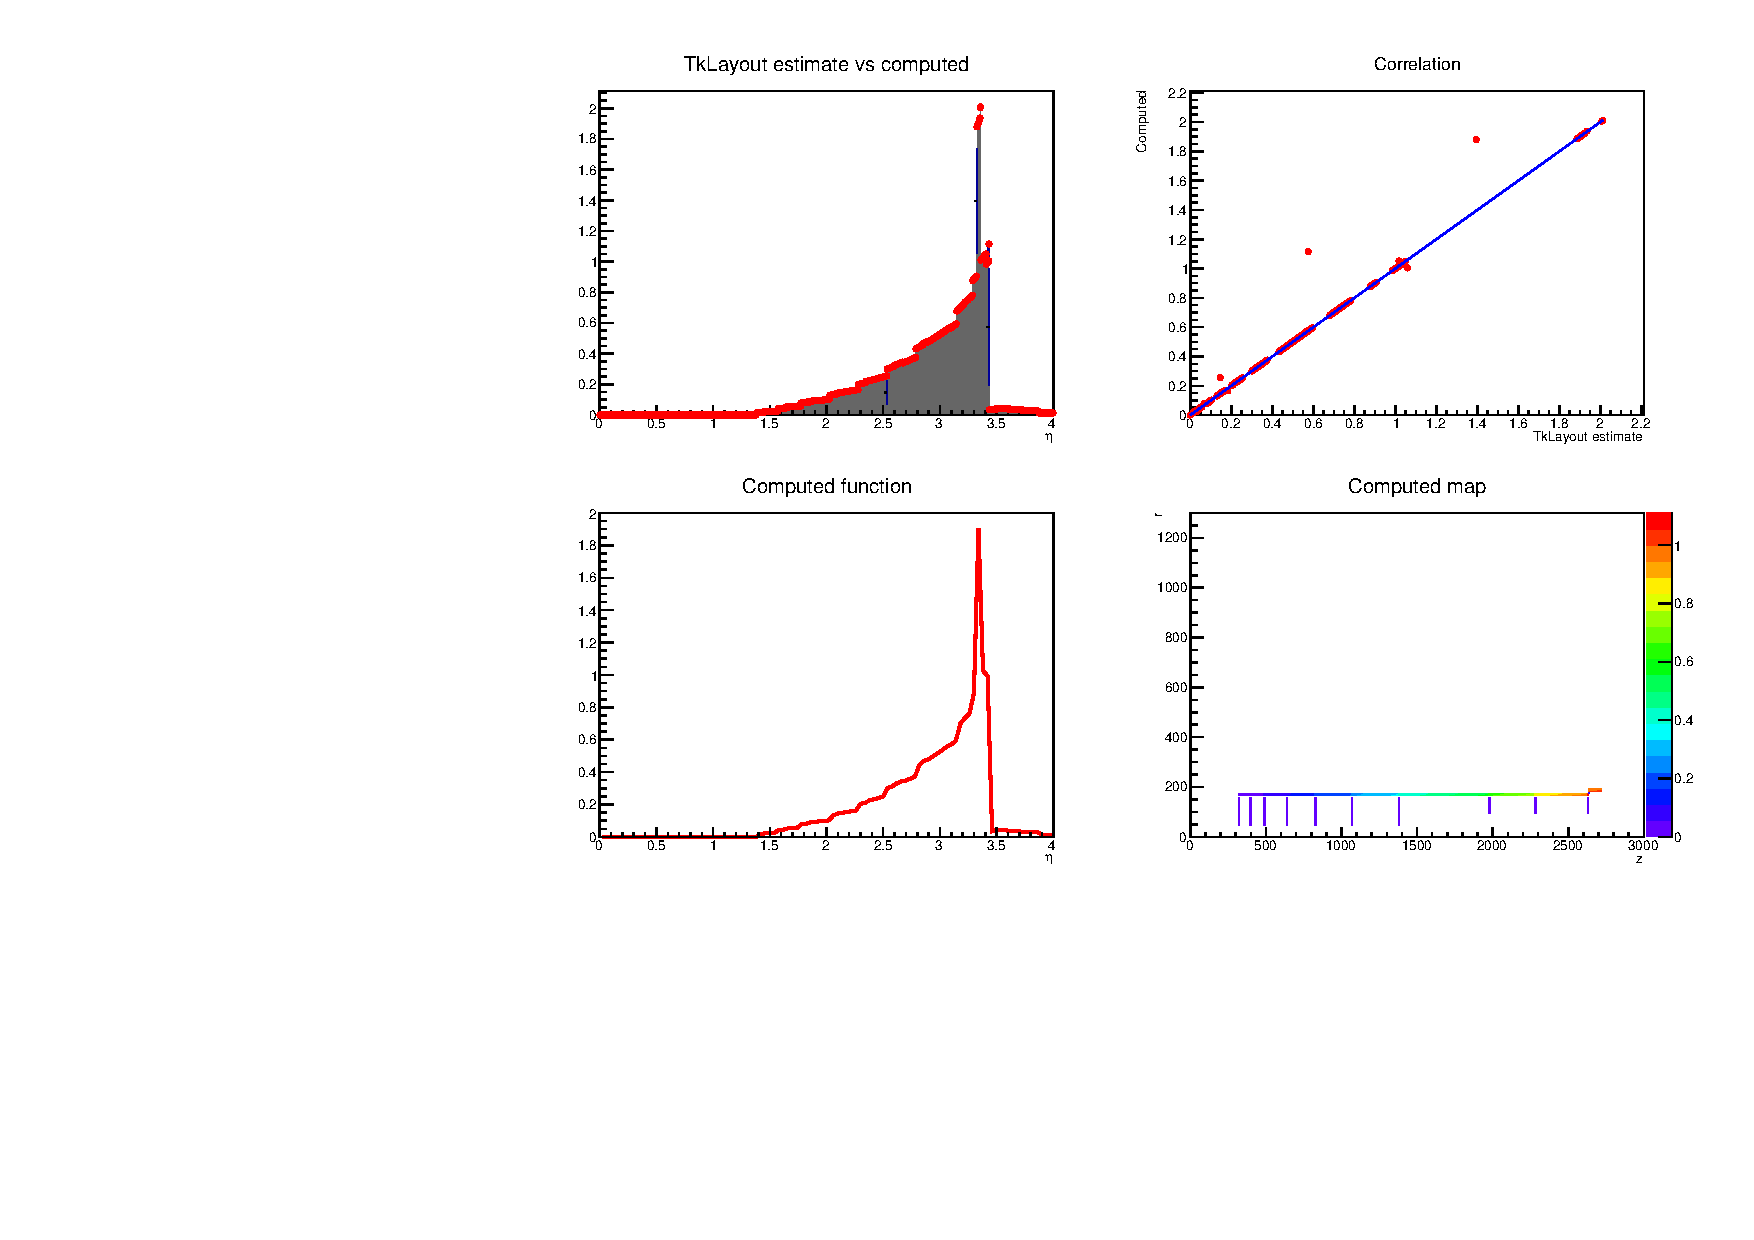
\includegraphics[width=9cm]{img/test12.pdf}
  \end{center}
\end{frame}

\begin{frame}
  \begin{block}{Test12bis}
    \alert{$0.1 mm$} of \emph{Cu} in the disks
    \begin{itemize}
    \item \alert{service} false
    \end{itemize}
  \end{block}
  \begin{center}
    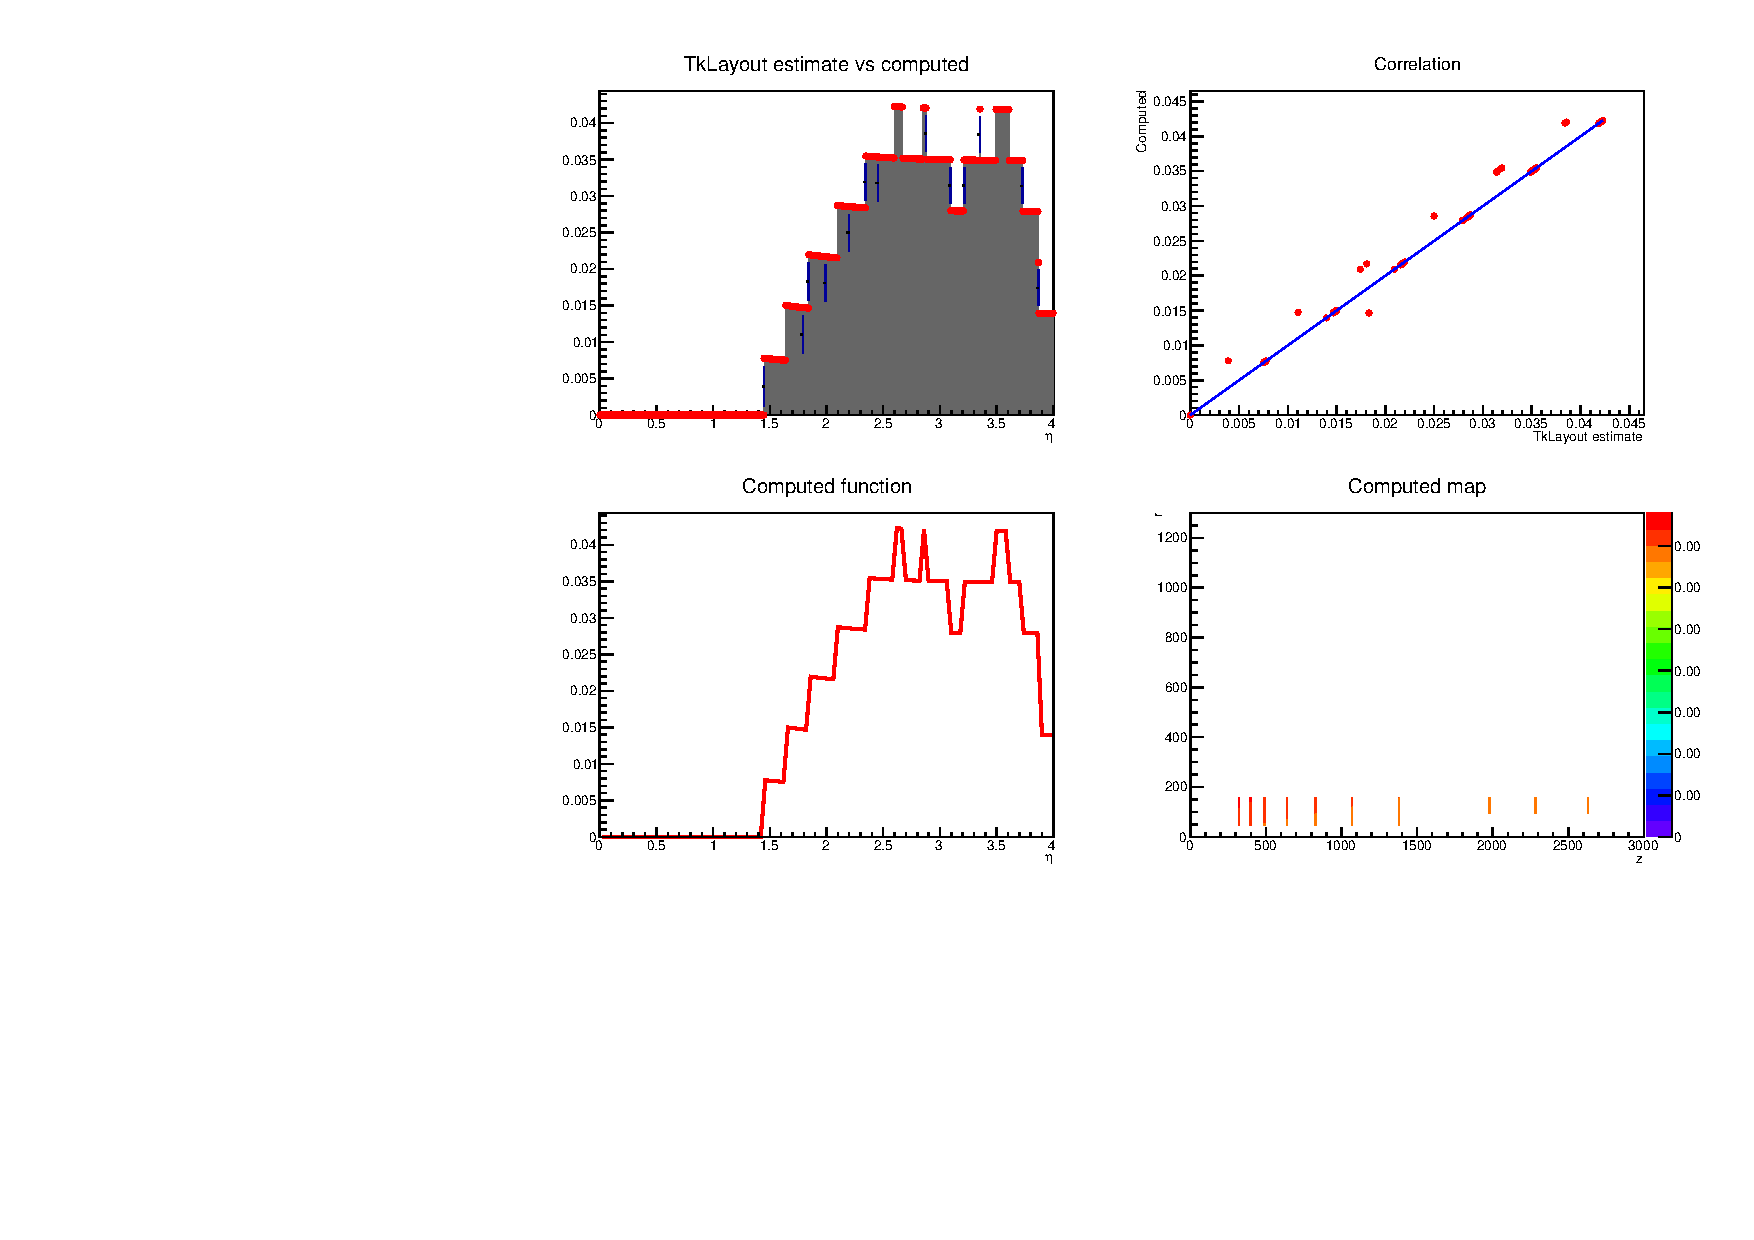
\includegraphics[width=9cm]{img/test12bis.pdf}
  \end{center}
\end{frame}

\begin{frame}
  \begin{block}{Test13}
    \alert{$0.1 mm$} of \emph{Cu} from the modules of disks
    \begin{itemize}
    \item \alert{service} true
    \end{itemize}
  \end{block}
  \begin{center}
    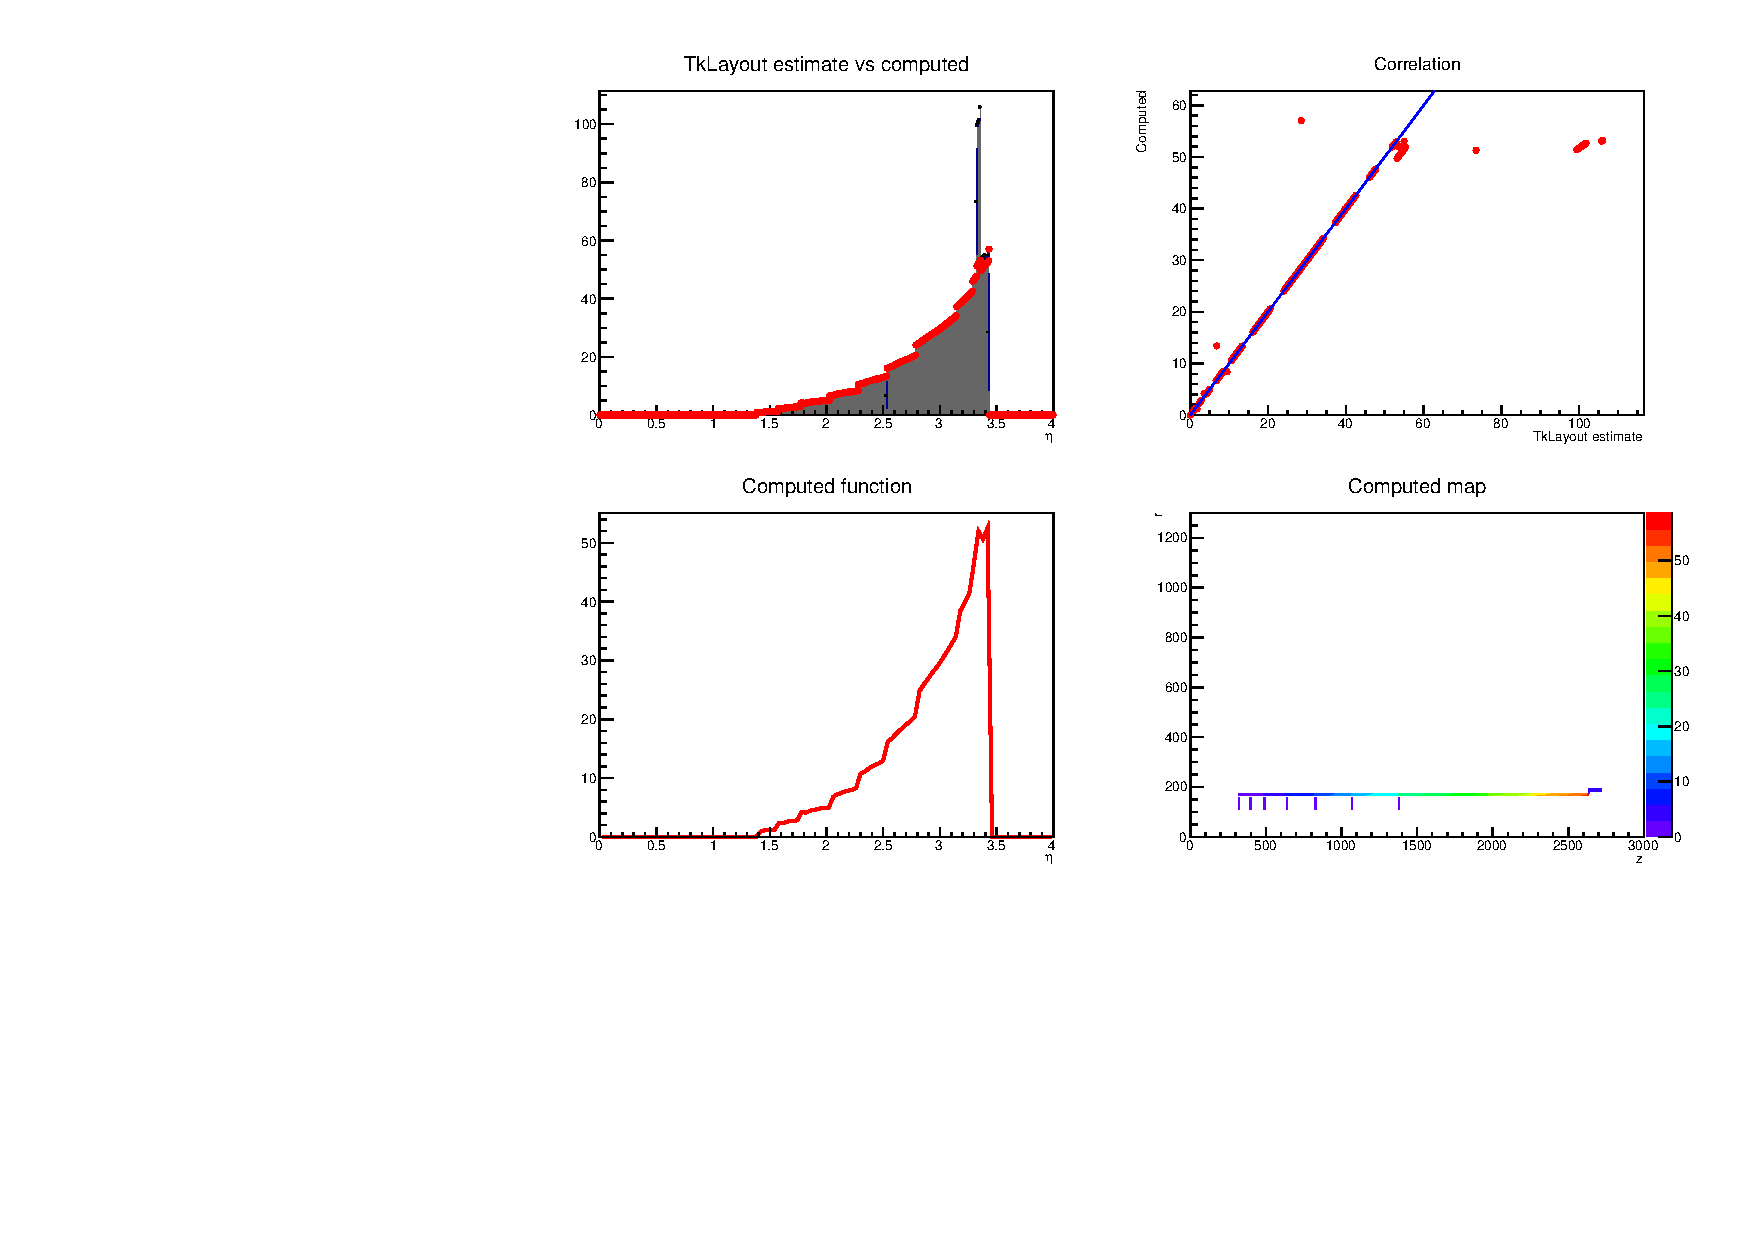
\includegraphics[width=9cm]{img/test13.pdf}
  \end{center}
\end{frame}

%% \begin{frame}
%%   \begin{block}{Test13bis}
%%     \alert{$0.1 mm$} of \emph{Cu} from the modules of the first disks
%%     \begin{itemize}
%%     \item \alert{service} true
%%     \end{itemize}
%%   \end{block}
%%   \begin{center}
%%     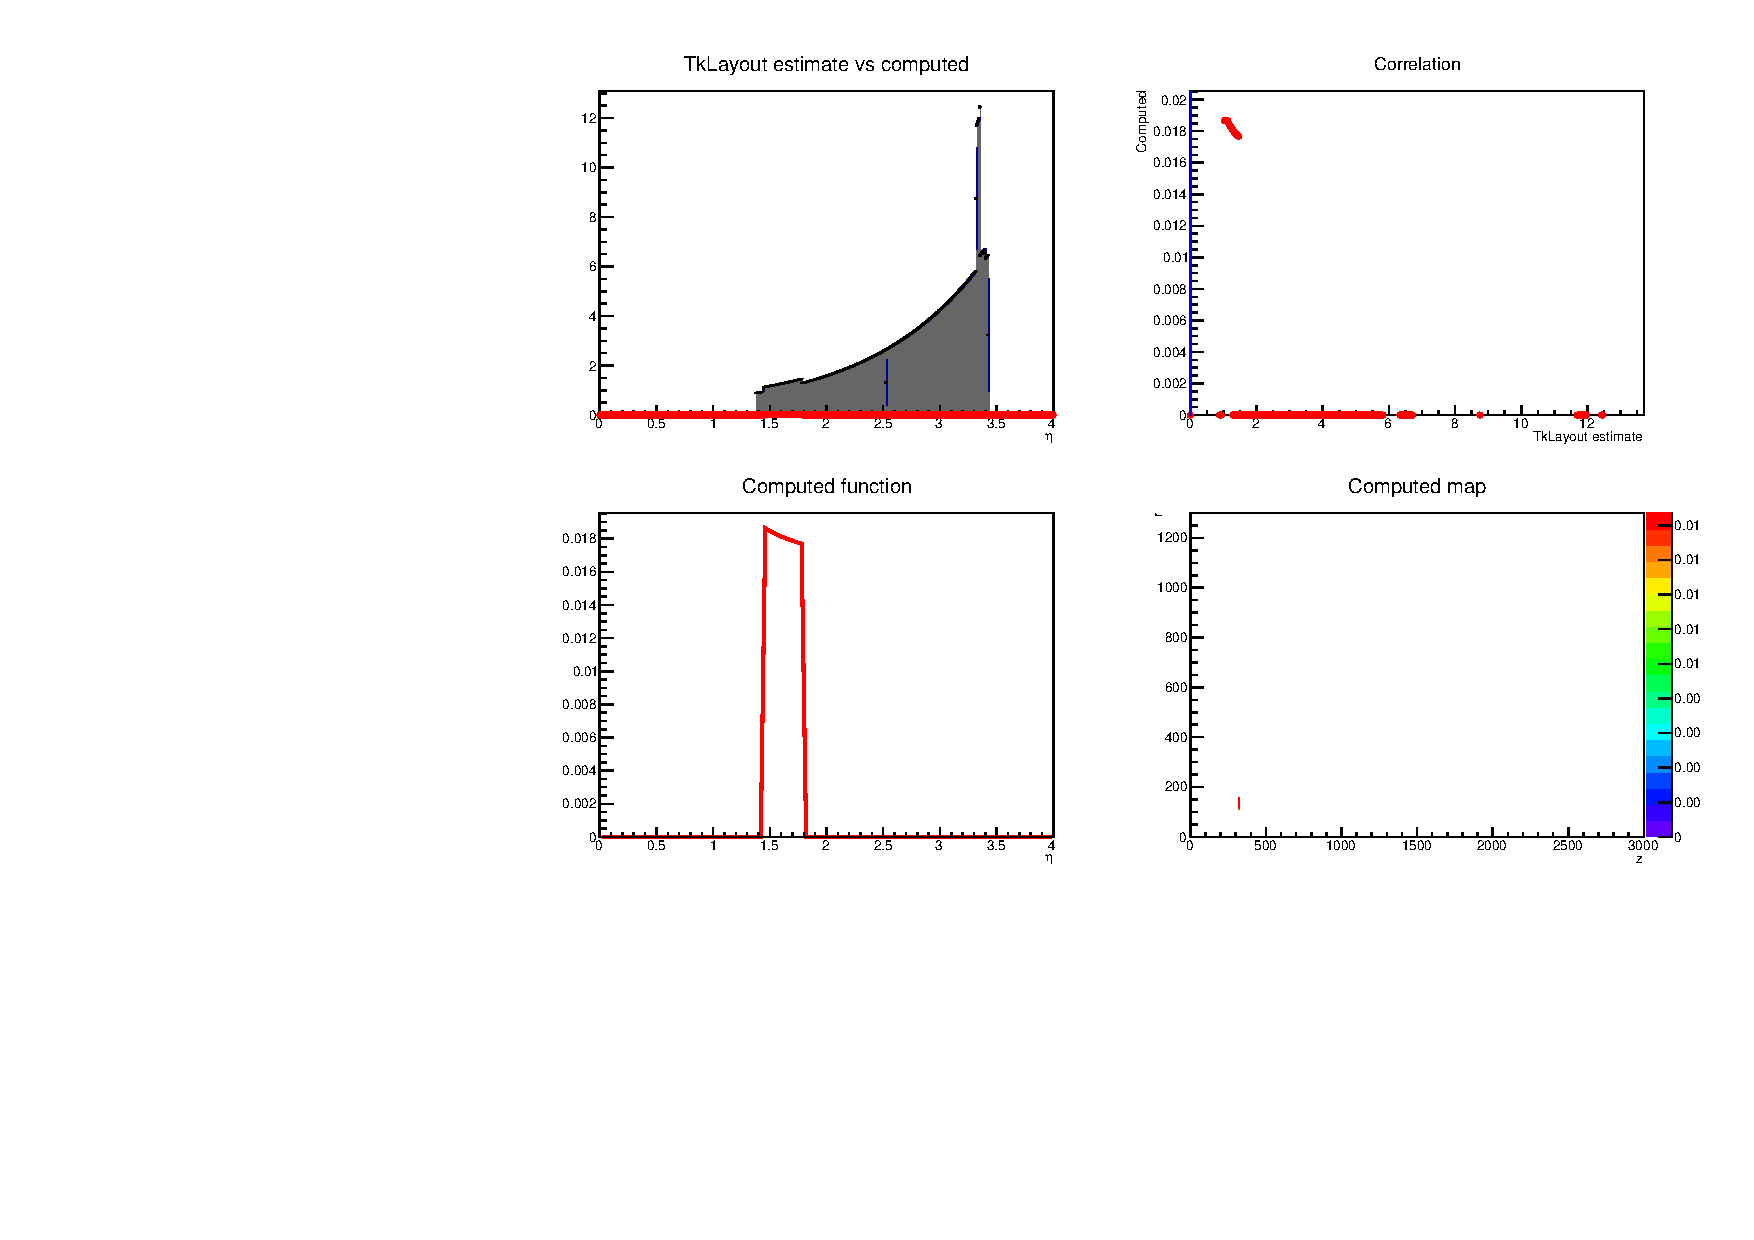
\includegraphics[width=9cm]{img/test13bis.pdf}
%%   \end{center}
%% \end{frame}

\begin{frame}
  \begin{block}{Test13b}
    \alert{$0.1 mm$} of \emph{Cu} from the modules of the first layer
    \begin{itemize}
    \item \alert{service} true
    \end{itemize}
  \end{block}
  \begin{center}
    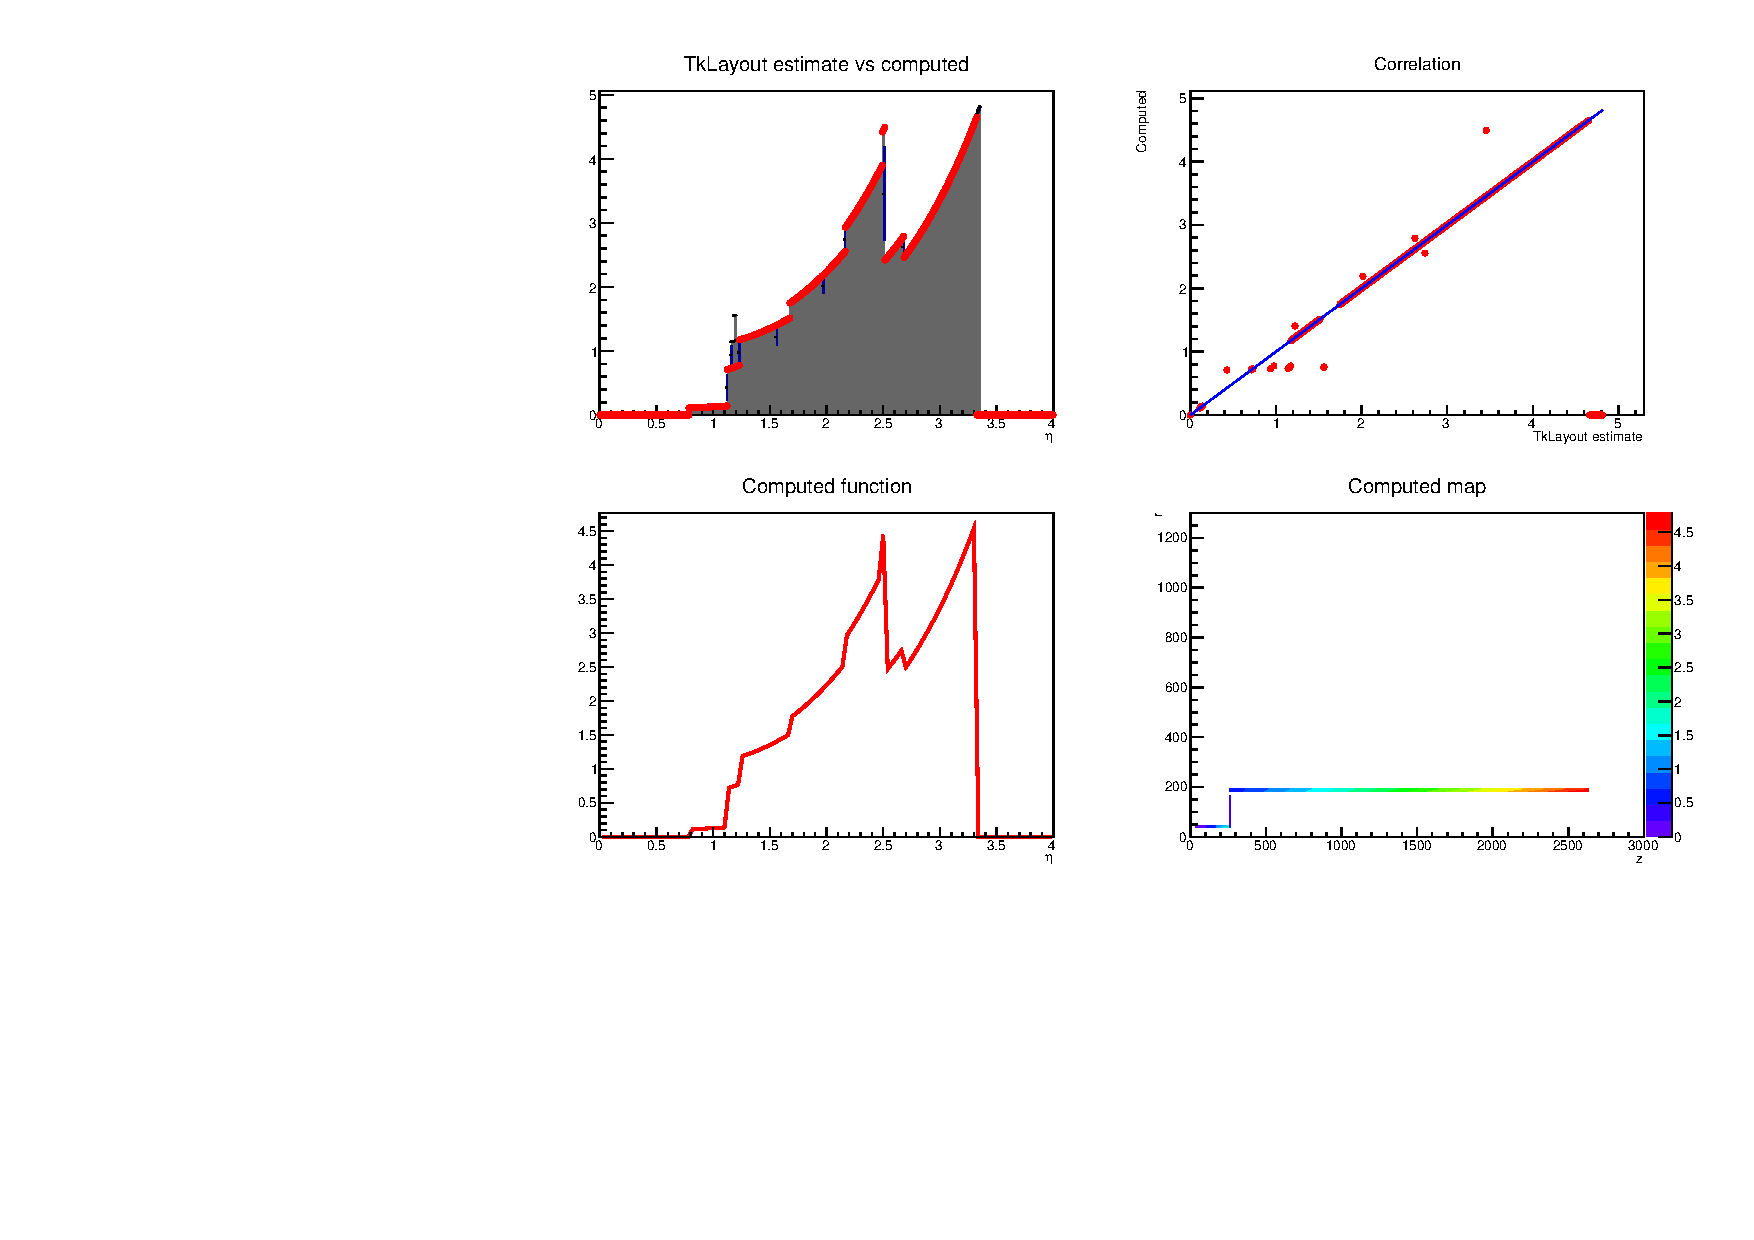
\includegraphics[width=9cm]{img/test13b.pdf}
  \end{center}
\end{frame}

\begin{frame}
  \begin{block}{Test14}
    \alert{$100 g/m$} of \emph{Cu} from the modules of the first disk
    \begin{itemize}
    \item \alert{service} true
    \end{itemize}
  \end{block}
  \begin{center}
    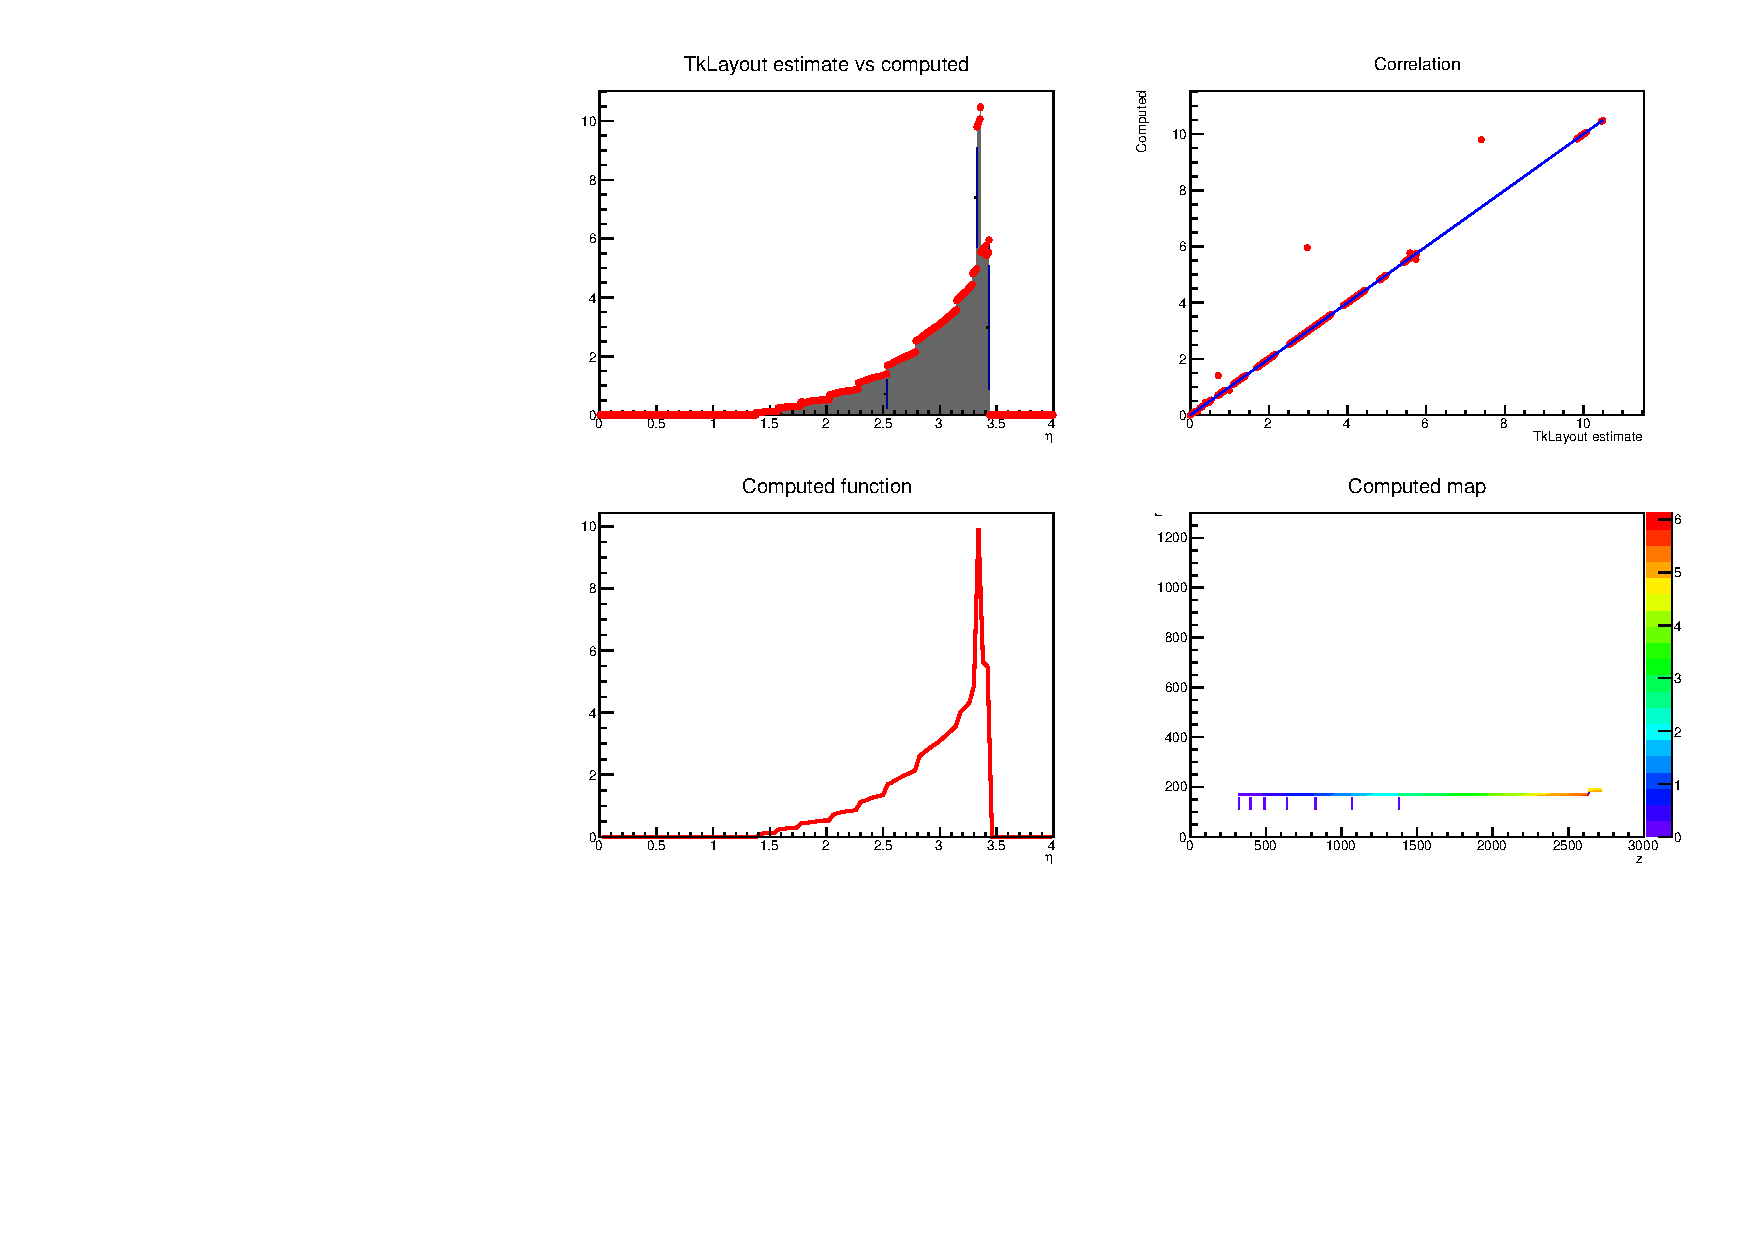
\includegraphics[width=9cm]{img/test14.pdf}
  \end{center}
\end{frame}

\begin{frame}
  \begin{block}{Test15}
    \alert{$100 g/m$} of \emph{Cu} in the disk of endcap
    \begin{itemize}
    \item \alert{service} true
    \end{itemize}
  \end{block}
  \begin{center}
    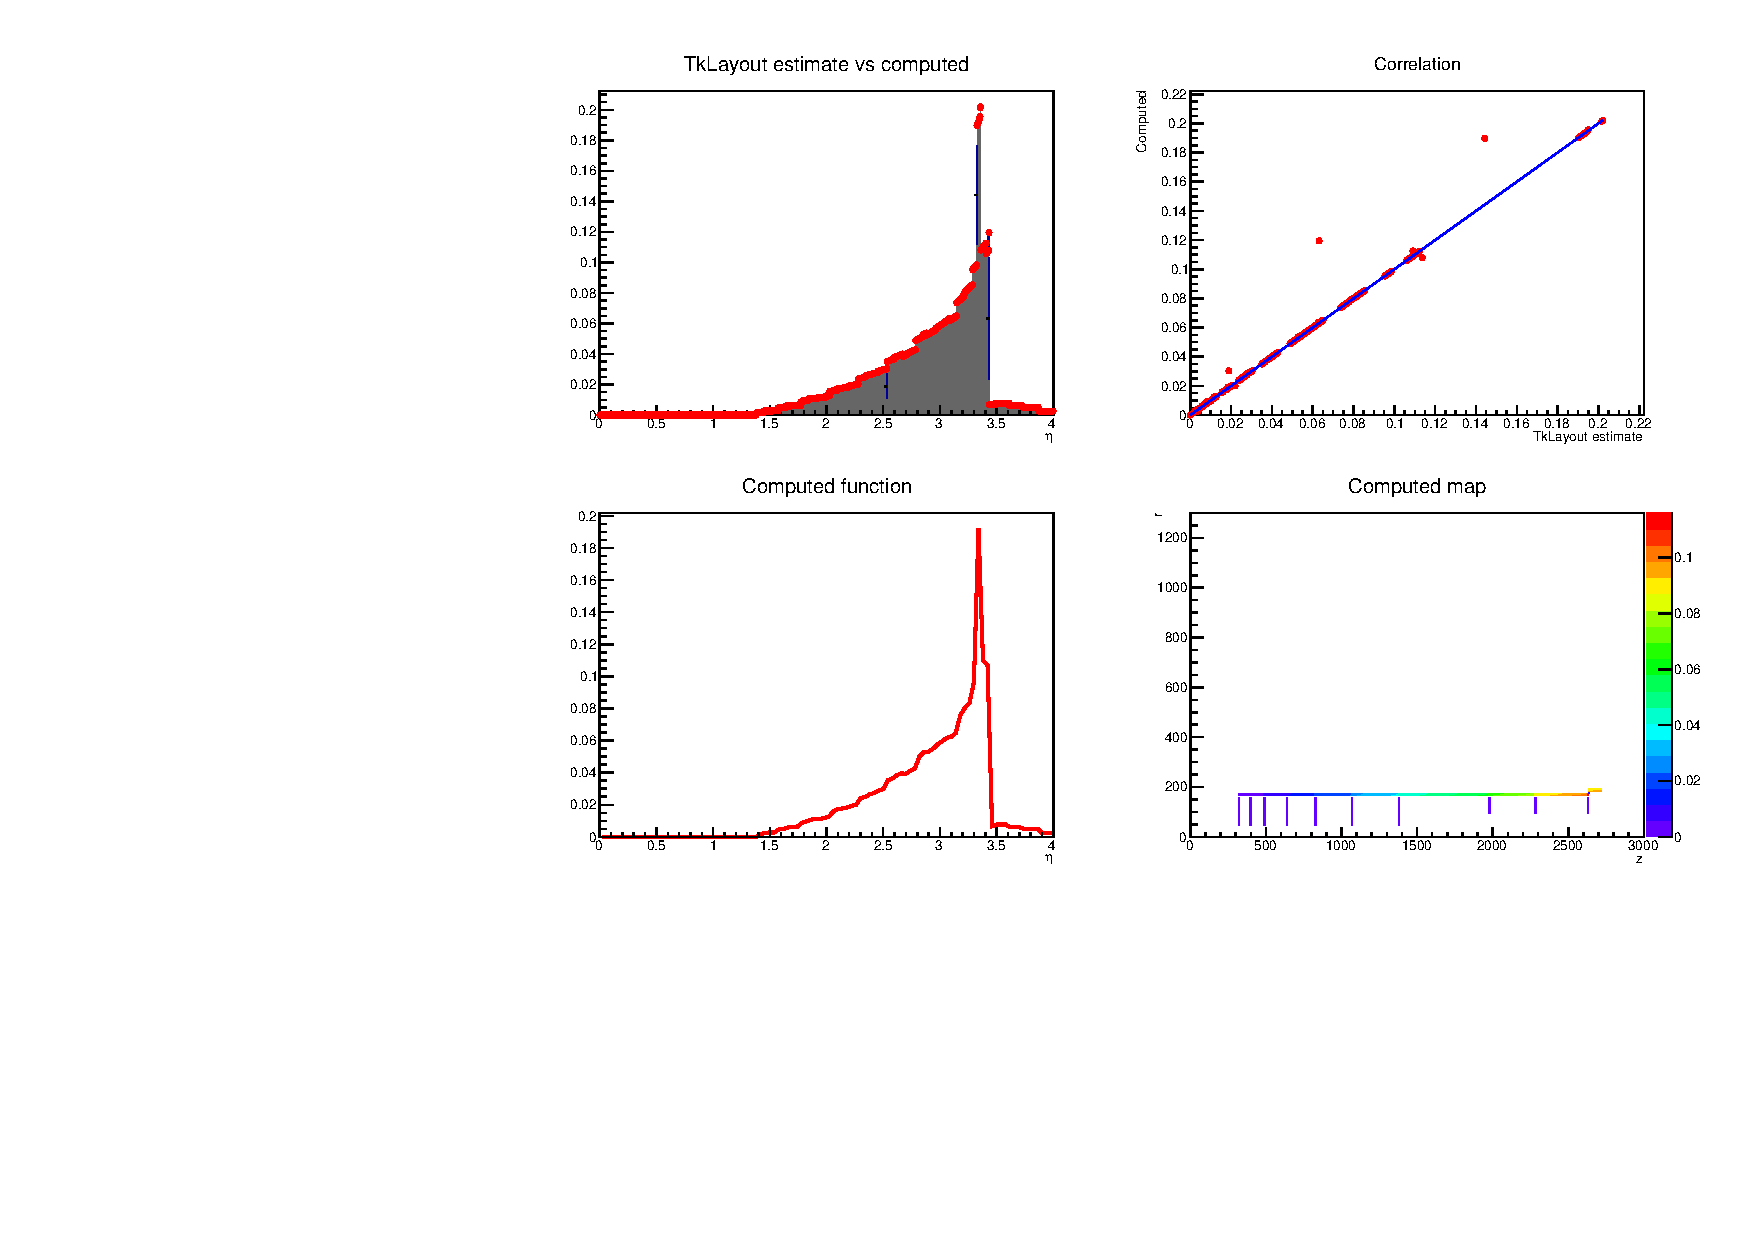
\includegraphics[width=9cm]{img/test15.pdf}
  \end{center}
\end{frame}

\begin{frame}
  \begin{block}{Test15bis}
    \alert{$100 g/m$} of \emph{Cu} in the disk of endcap
    \begin{itemize}
    \item \alert{service} false
    \end{itemize}
  \end{block}
  \begin{center}
    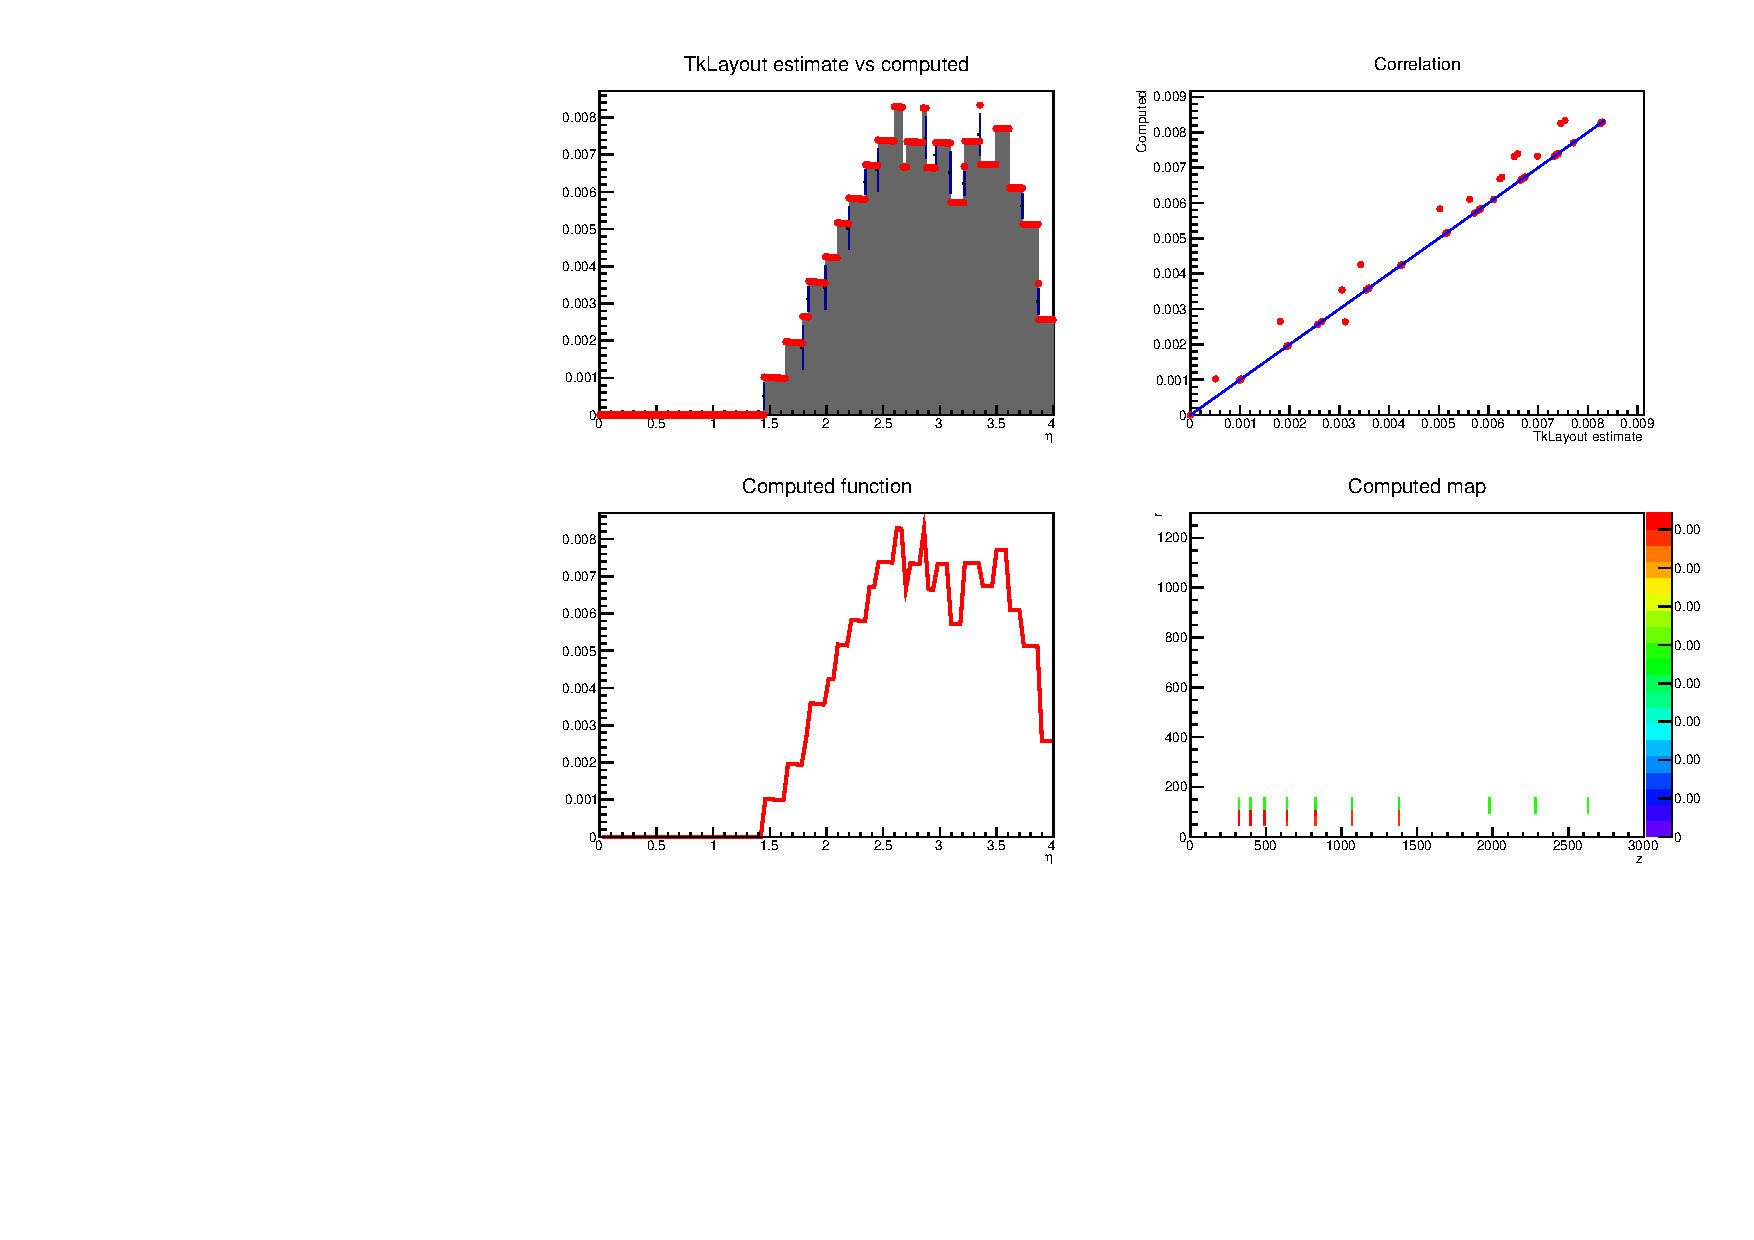
\includegraphics[width=9cm]{img/test15bis.pdf}
  \end{center}
\end{frame}

\begin{frame}
  \begin{block}{Test16}
    \alert{$10 g$} of \emph{Cu} in the disk of endcap
    \begin{itemize}
    \item \alert{service} false
    \end{itemize}
  \end{block}
  \begin{center}
    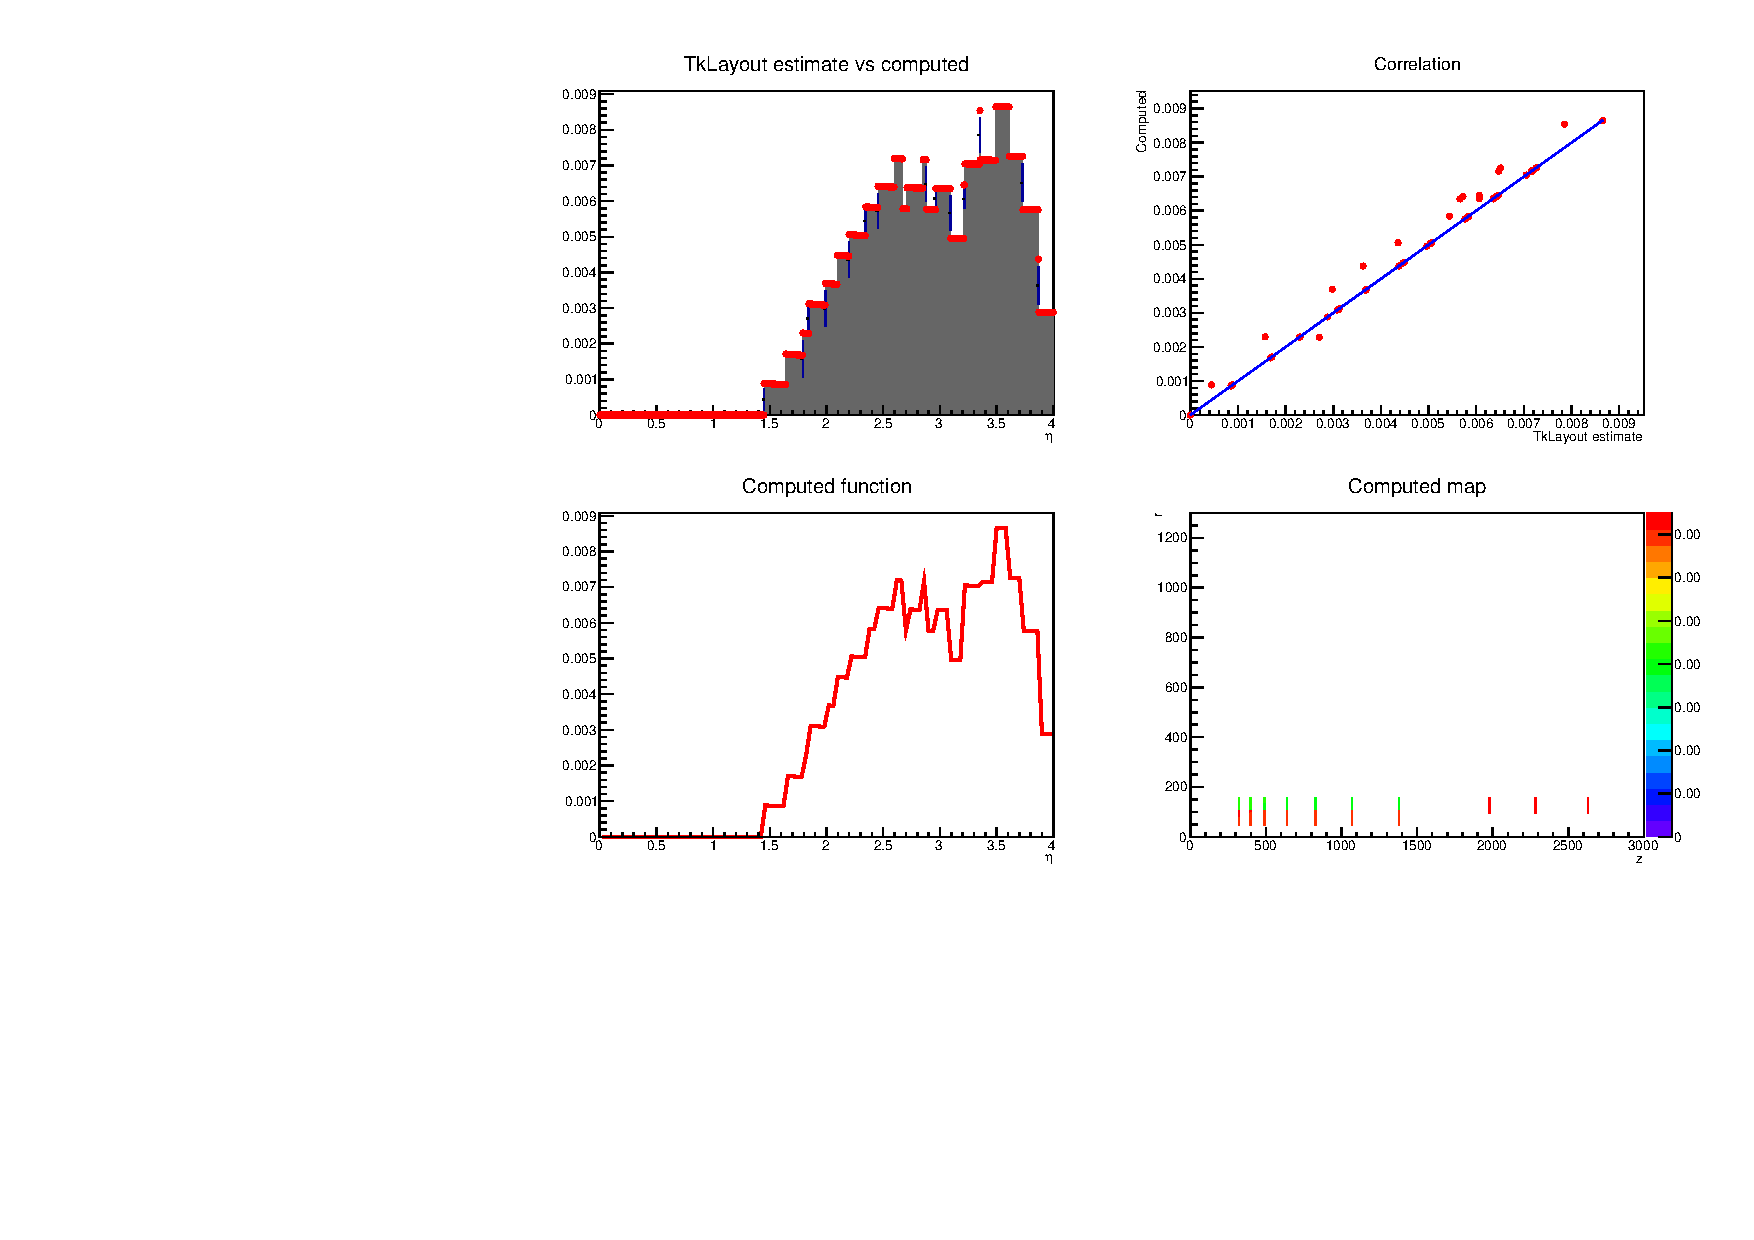
\includegraphics[width=9cm]{img/test16.pdf}
  \end{center}
\end{frame}

\begin{frame}
  \begin{block}{Test17}
    \alert{$10 g$} of \emph{Cu} in the layers of barrel
    \begin{itemize}
    \item \alert{service} false
    \end{itemize}
  \end{block}
  \begin{center}
    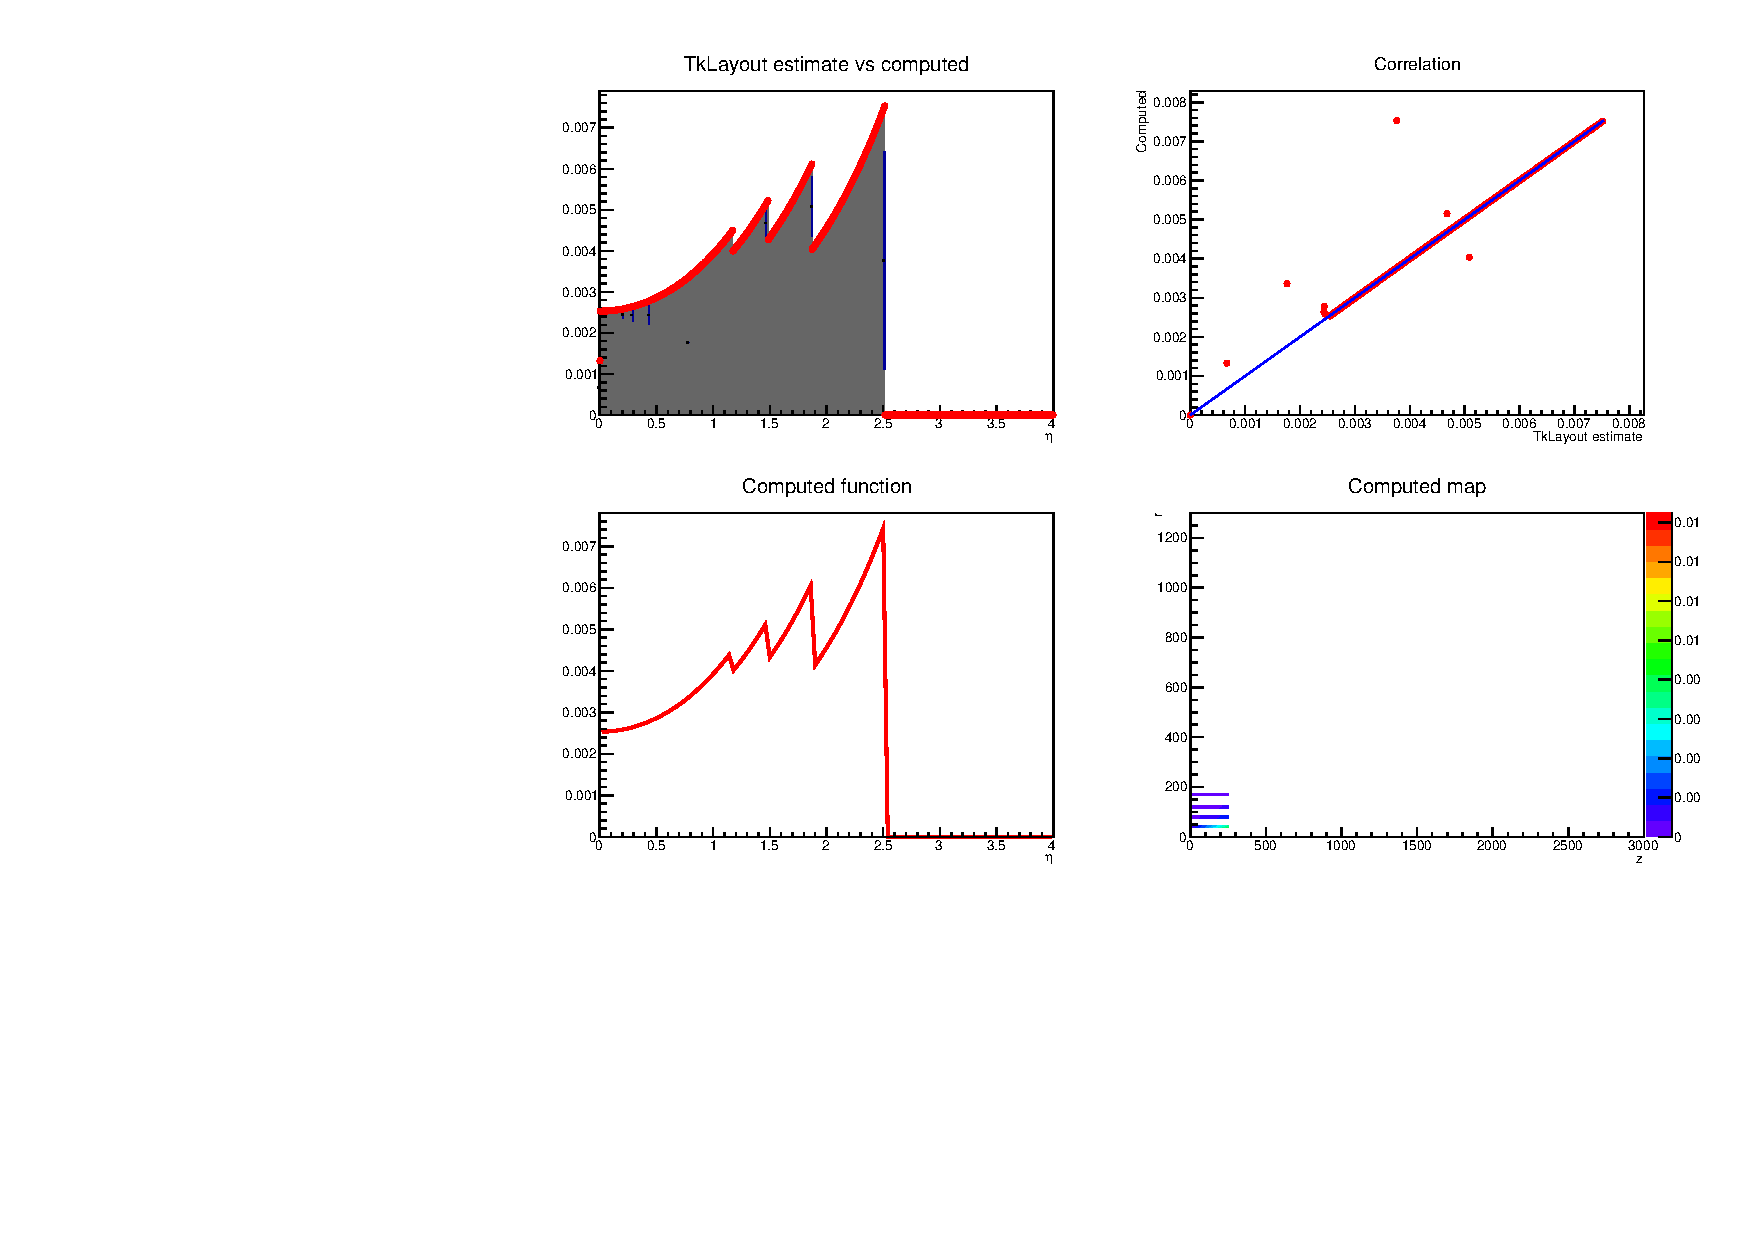
\includegraphics[width=9cm]{img/test17.pdf}
  \end{center}
\end{frame}

\begin{frame}
  \begin{block}{Test18}
    \alert{$0.1 mm$} of \emph{Cu} in the layers of barrel
    \begin{itemize}
    \item \alert{service} false
    \end{itemize}
  \end{block}
  \begin{center}
    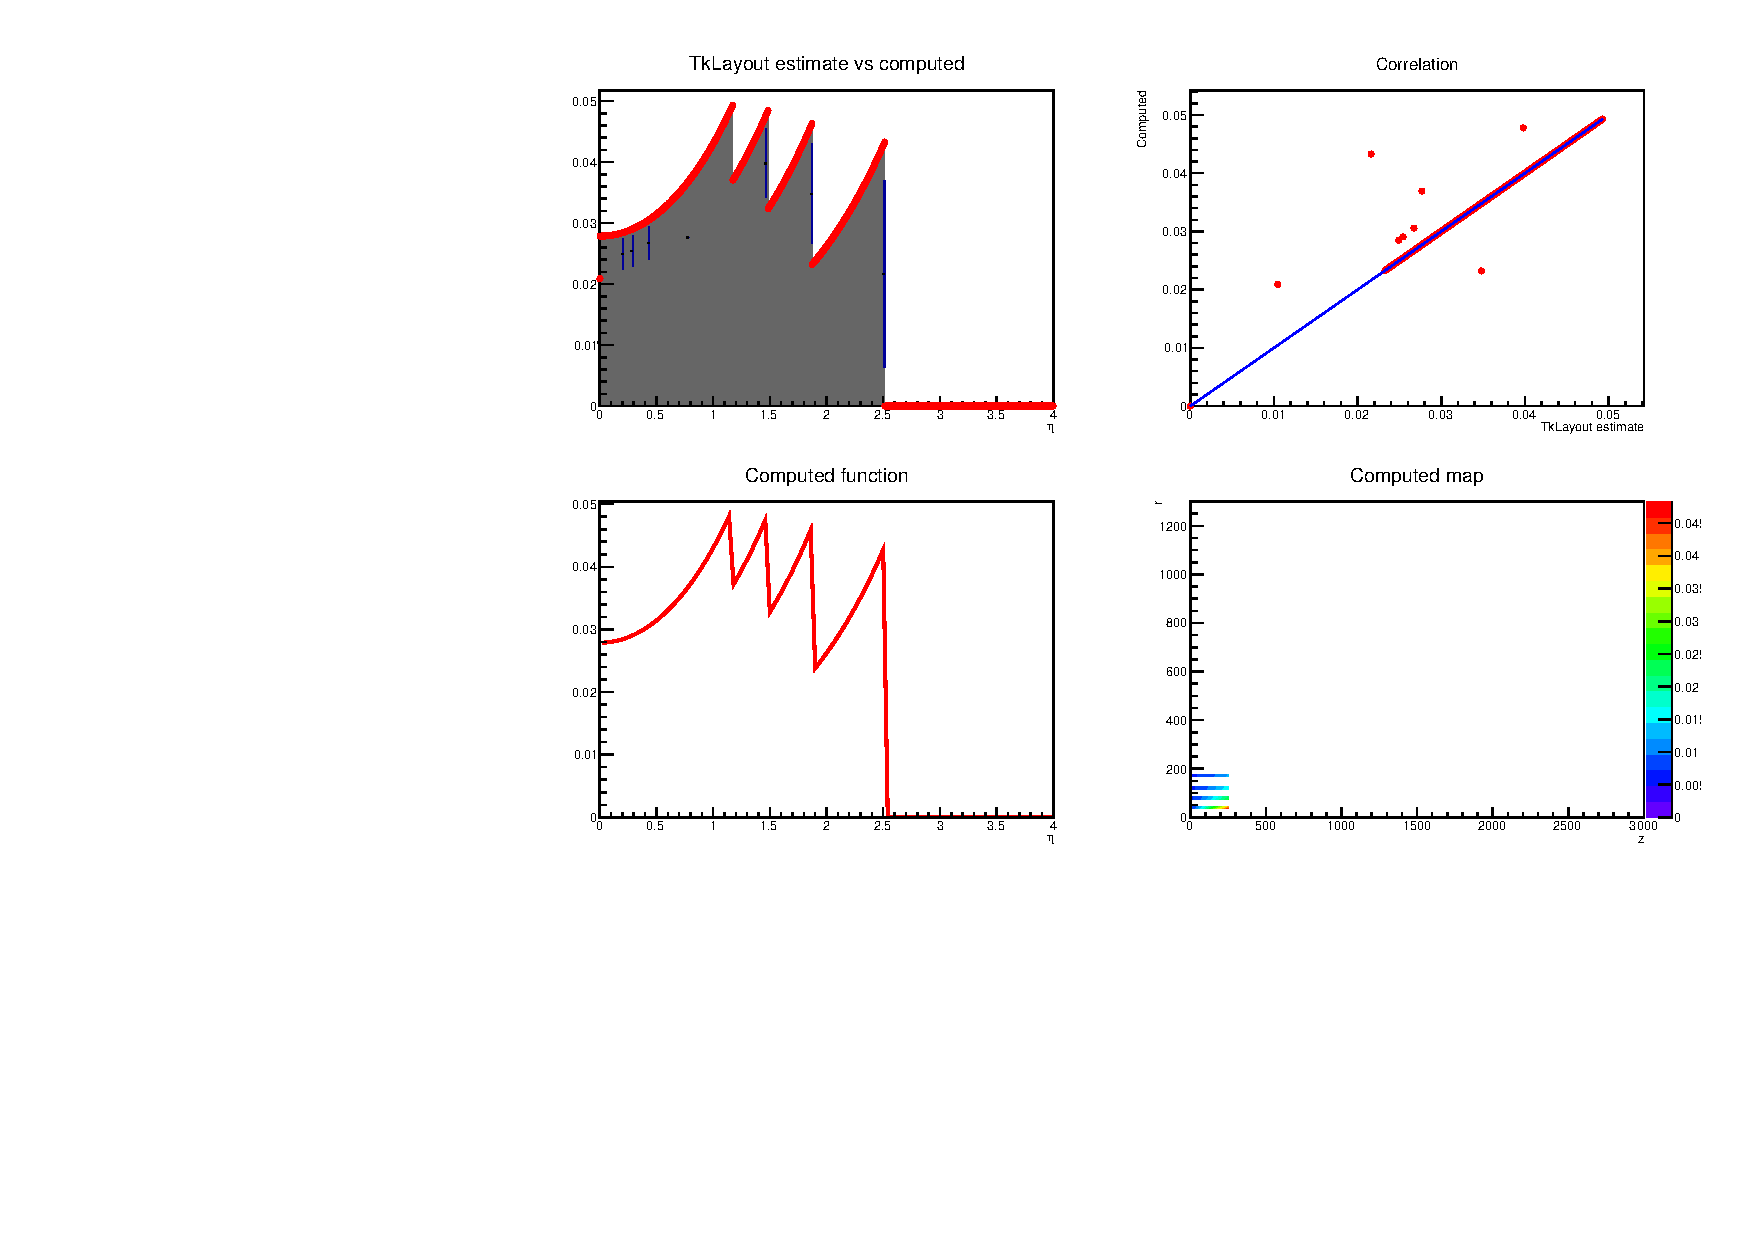
\includegraphics[width=9cm]{img/test18.pdf}
  \end{center}
\end{frame}

\begin{frame}
  \begin{block}{Test18bis}
    \alert{$0.1 mm$} of \emph{Cu} in the layers of barrel
    \begin{itemize}
    \item \alert{service} true
    \end{itemize}
  \end{block}
  \begin{center}
    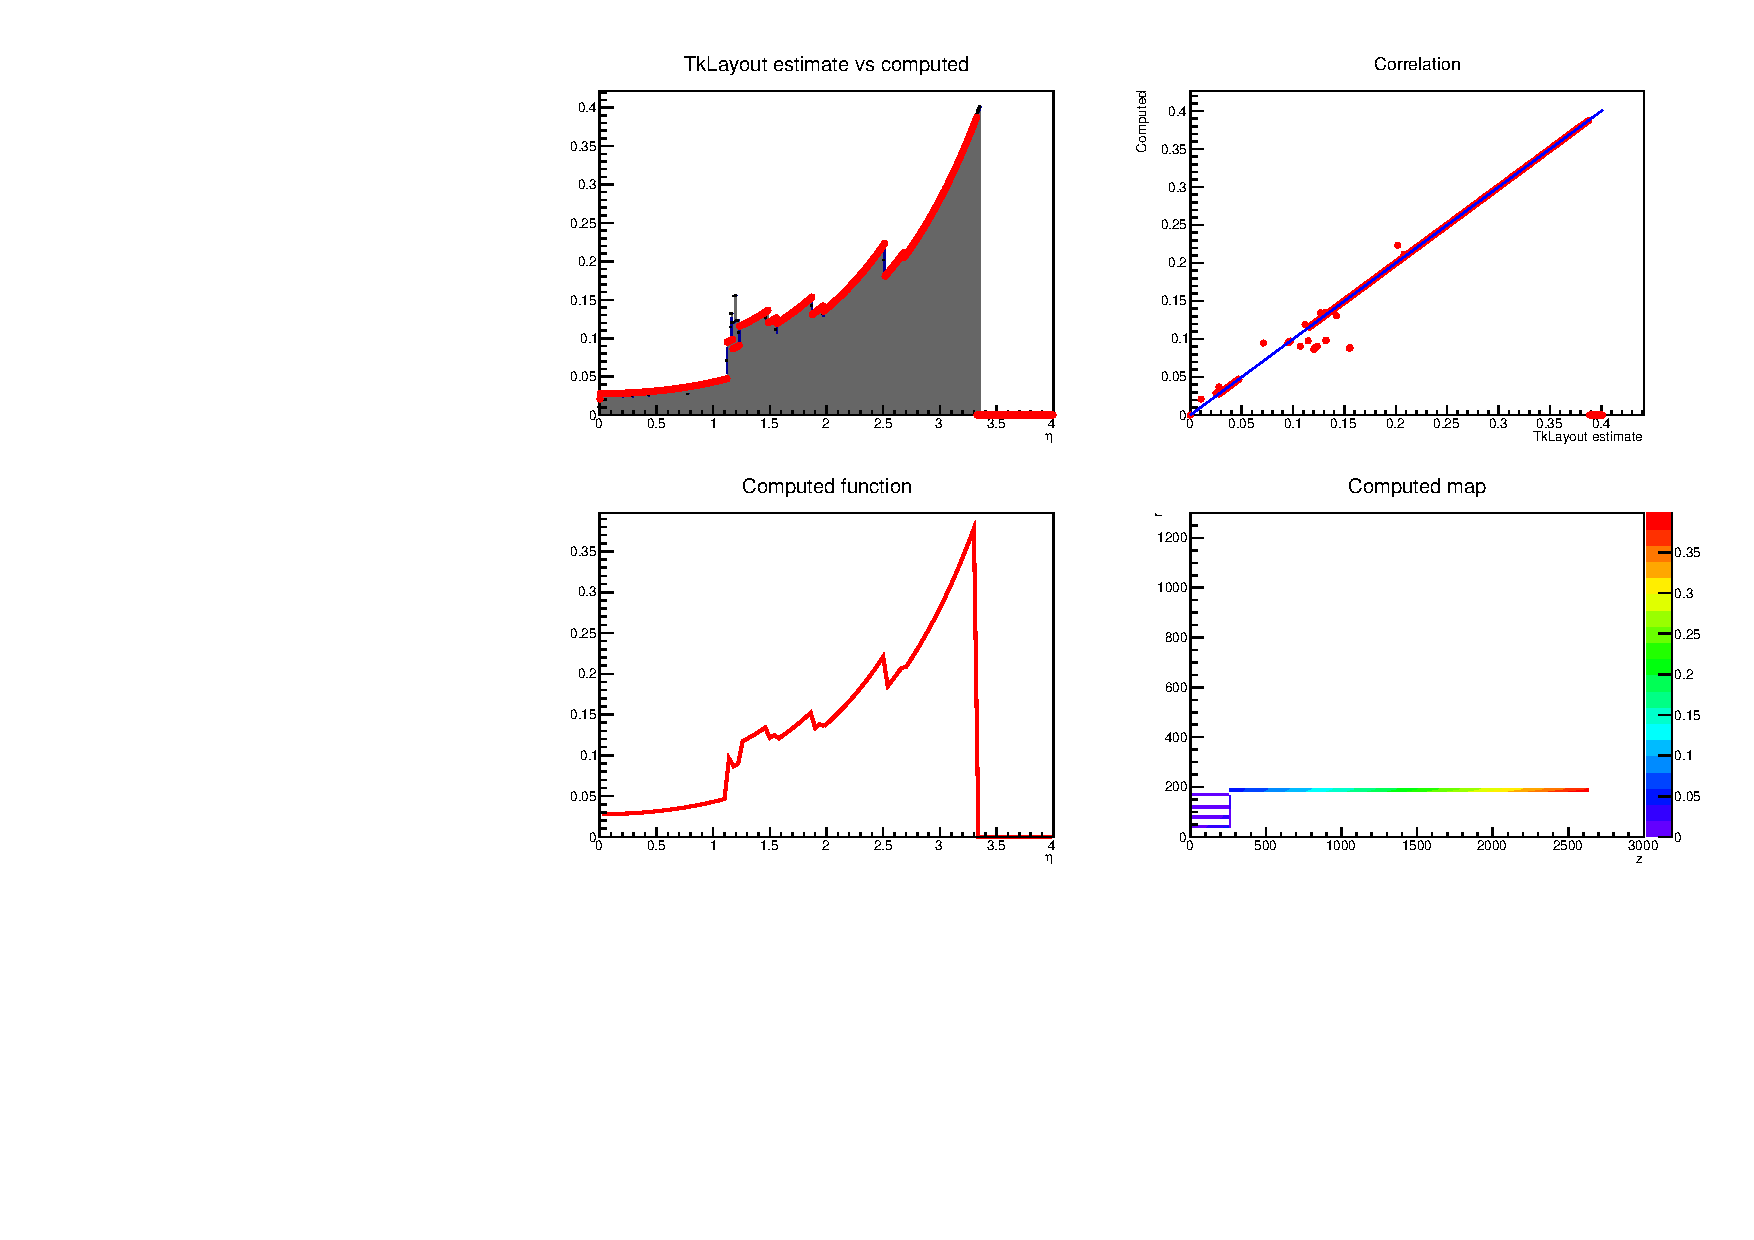
\includegraphics[width=9cm]{img/test18bis.pdf}
  \end{center}
\end{frame}

\begin{frame}
  \begin{block}{Test19}
    \alert{$100 g/m$} of \emph{Cu} in the layers of barrel
    \begin{itemize}
    \item \alert{service} false
    \end{itemize}
  \end{block}
  \begin{center}
    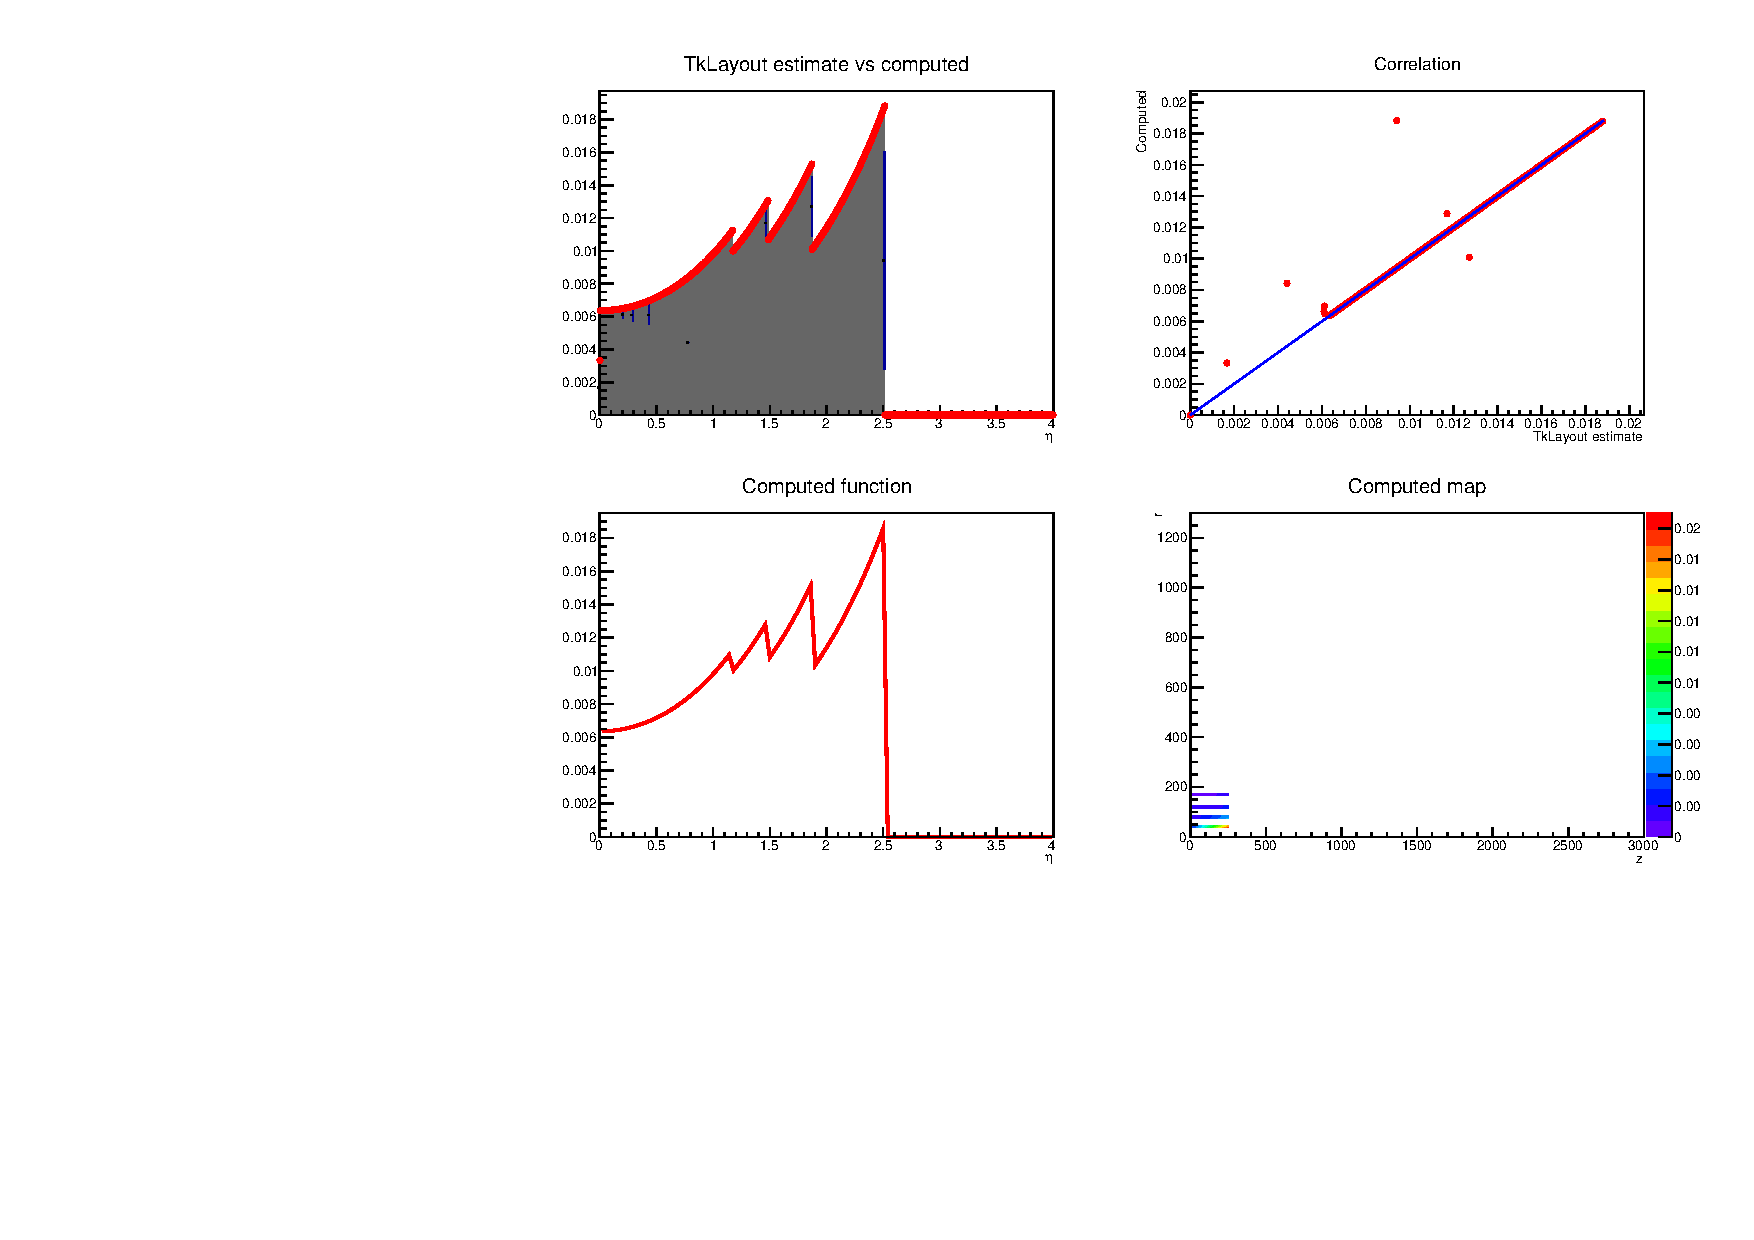
\includegraphics[width=9cm]{img/test19.pdf}
  \end{center}
\end{frame}

\begin{frame}
  \begin{block}{Test19bis}
    \alert{$100 g/m$} of \emph{Cu} in the layers of barrel
    \begin{itemize}
    \item \alert{service} true
    \end{itemize}
  \end{block}
  \begin{center}
    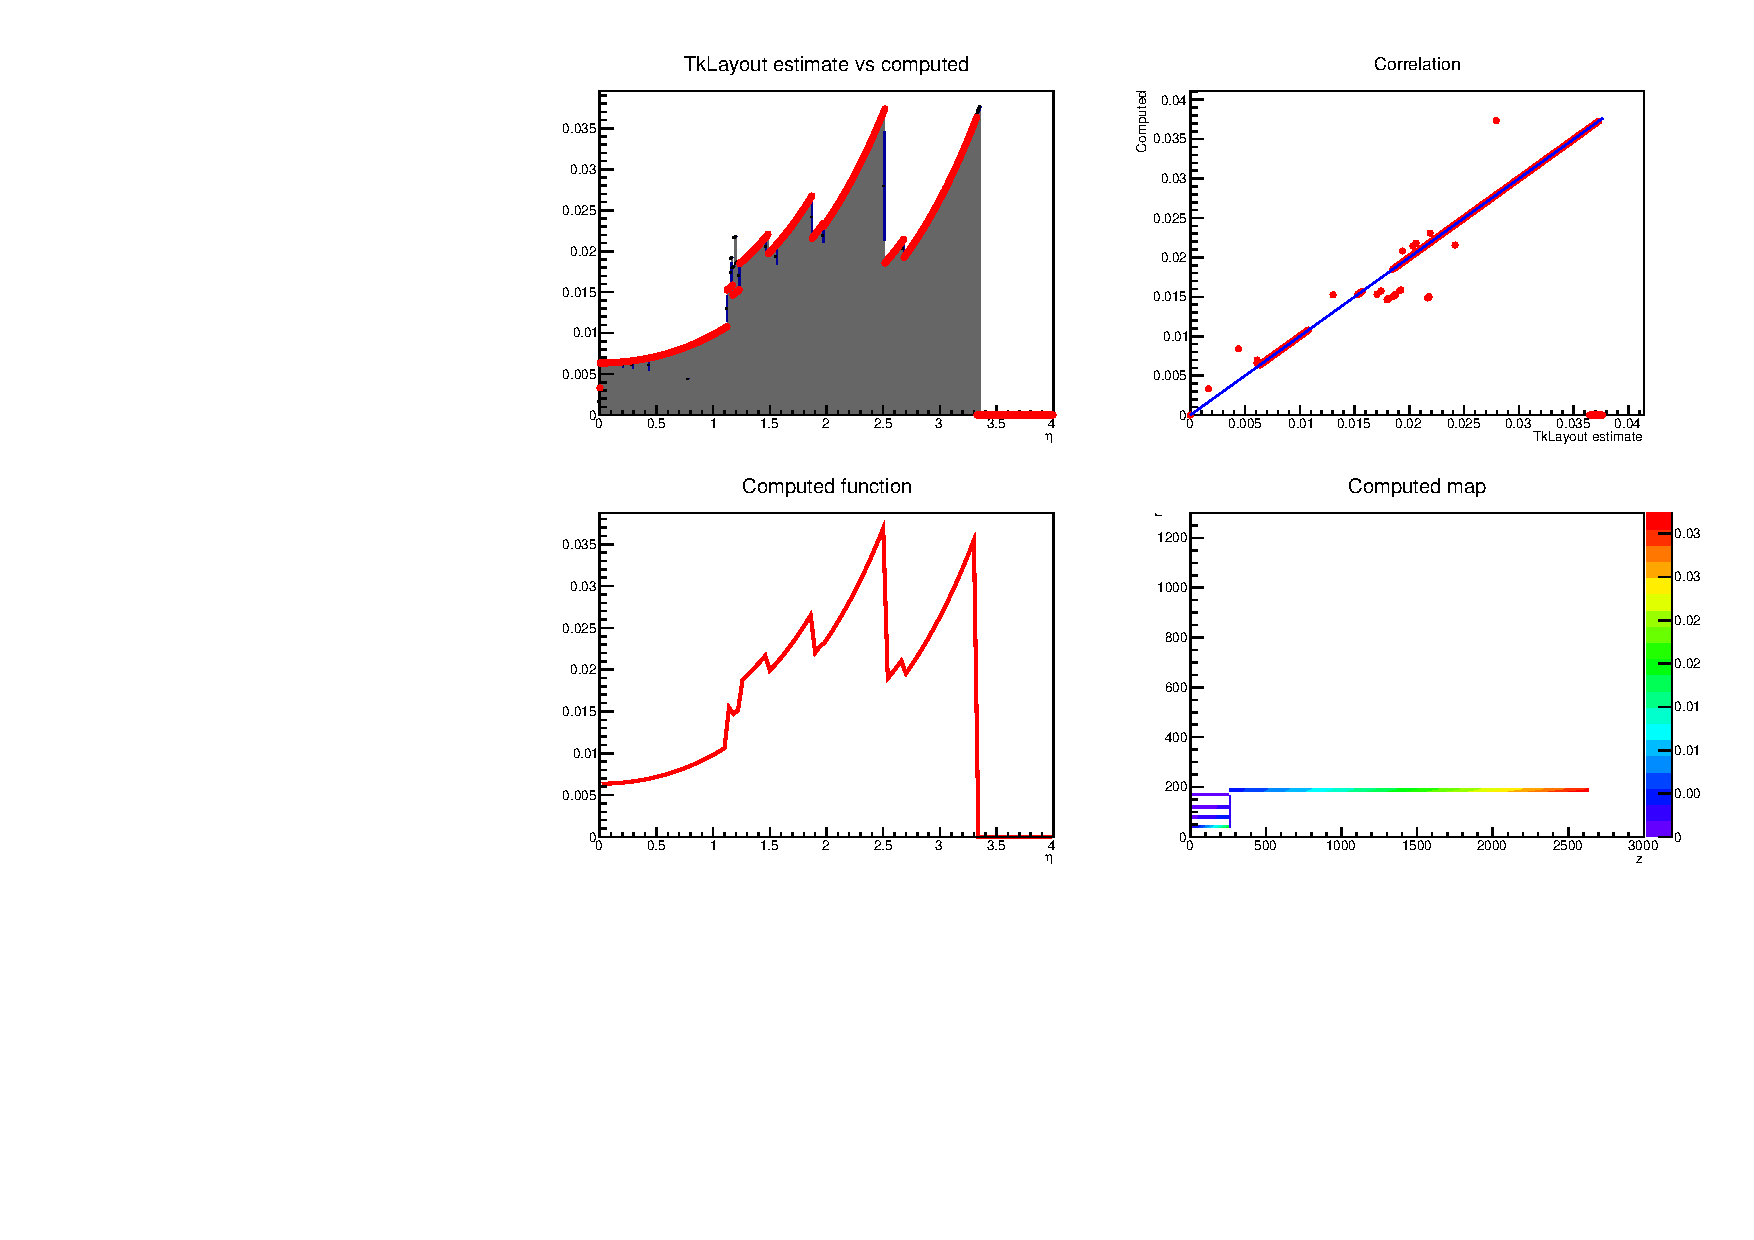
\includegraphics[width=9cm]{img/test19bis.pdf}
  \end{center}
\end{frame}

\begin{frame}
  \begin{block}{Test20}
    \alert{$100 g/m$} of \emph{Cu} in the rods of barrel
    \begin{itemize}
    \item \alert{service} false
    \end{itemize}
  \end{block}
  \begin{center}
    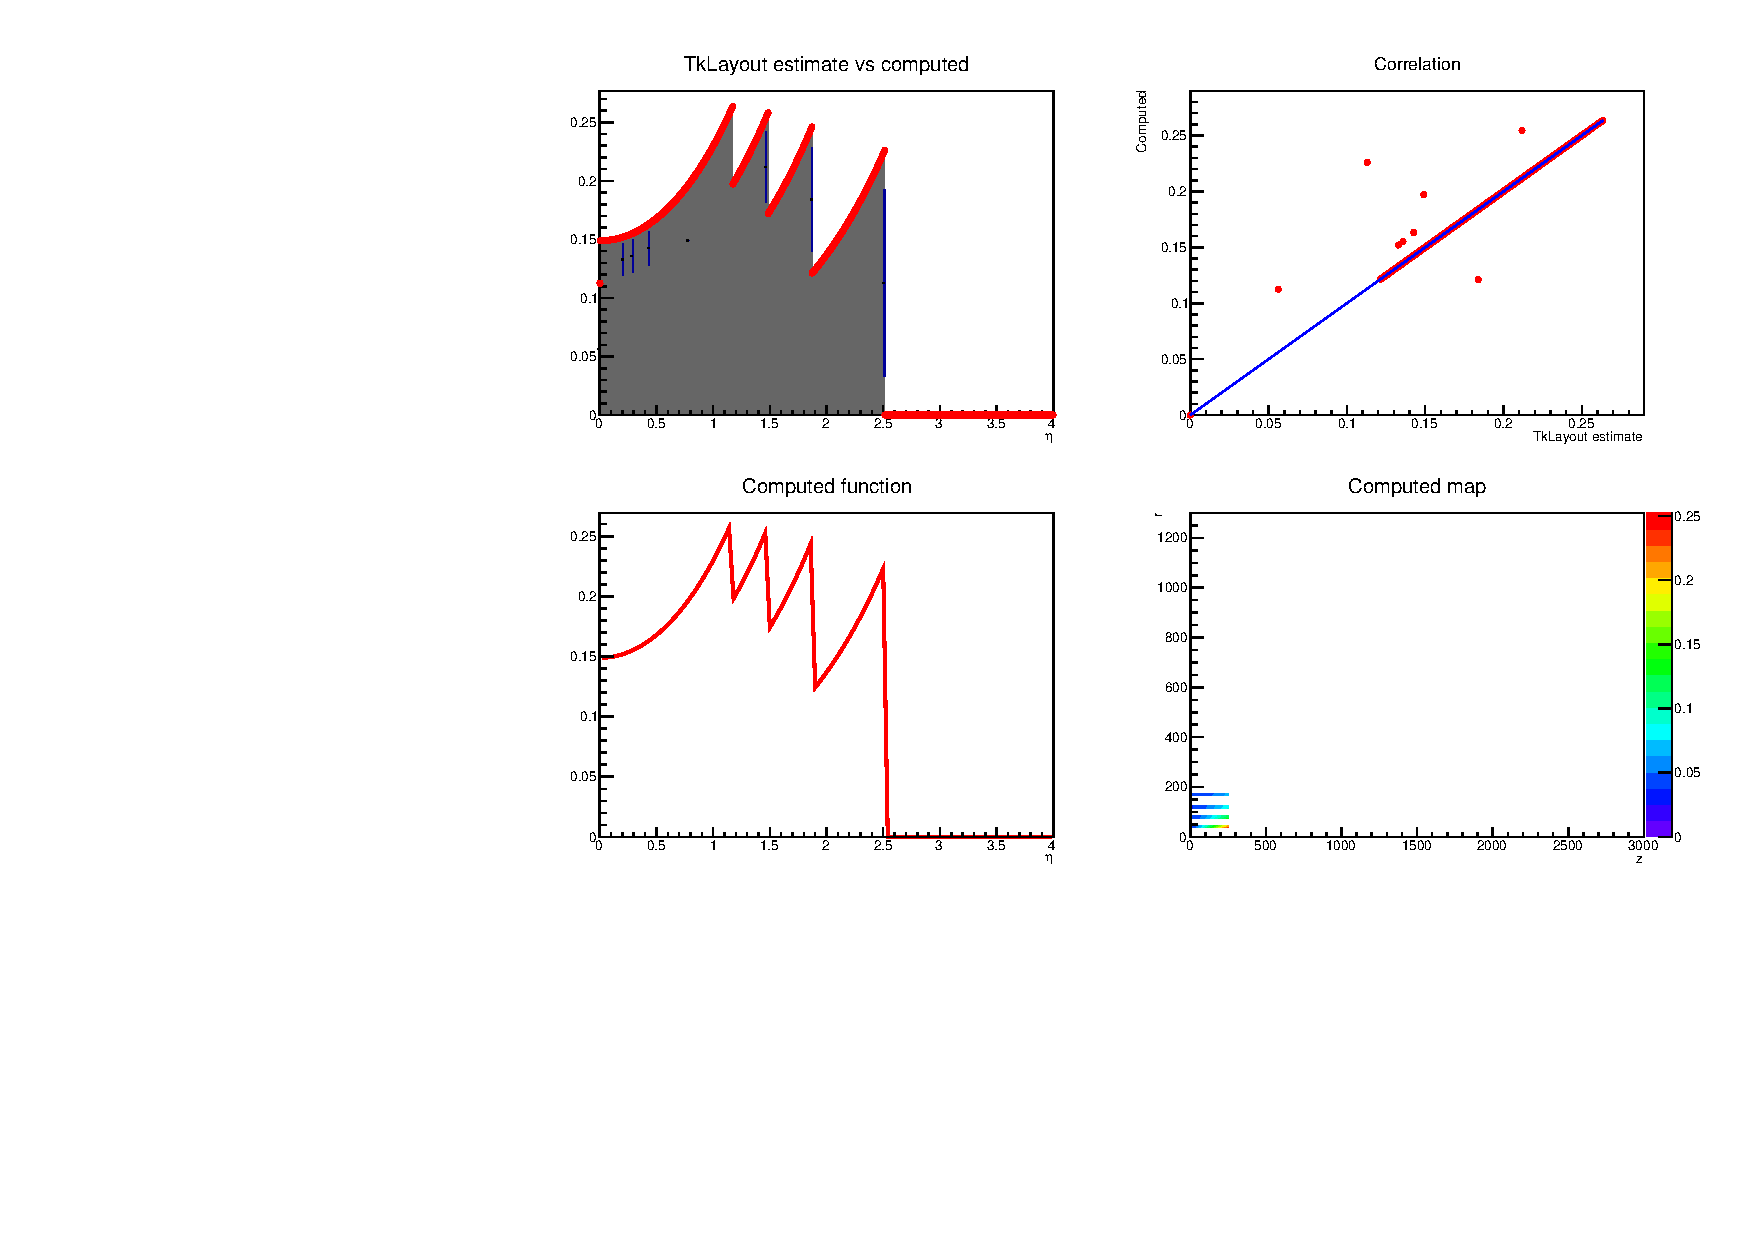
\includegraphics[width=9cm]{img/test20.pdf}
  \end{center}
\end{frame}

\begin{frame}
  \begin{block}{Test21}
    \alert{$10 g$} of \emph{Cu} in the rods of barrel
    \begin{itemize}
    \item \alert{service} false
    \end{itemize}
  \end{block}
  \begin{center}
    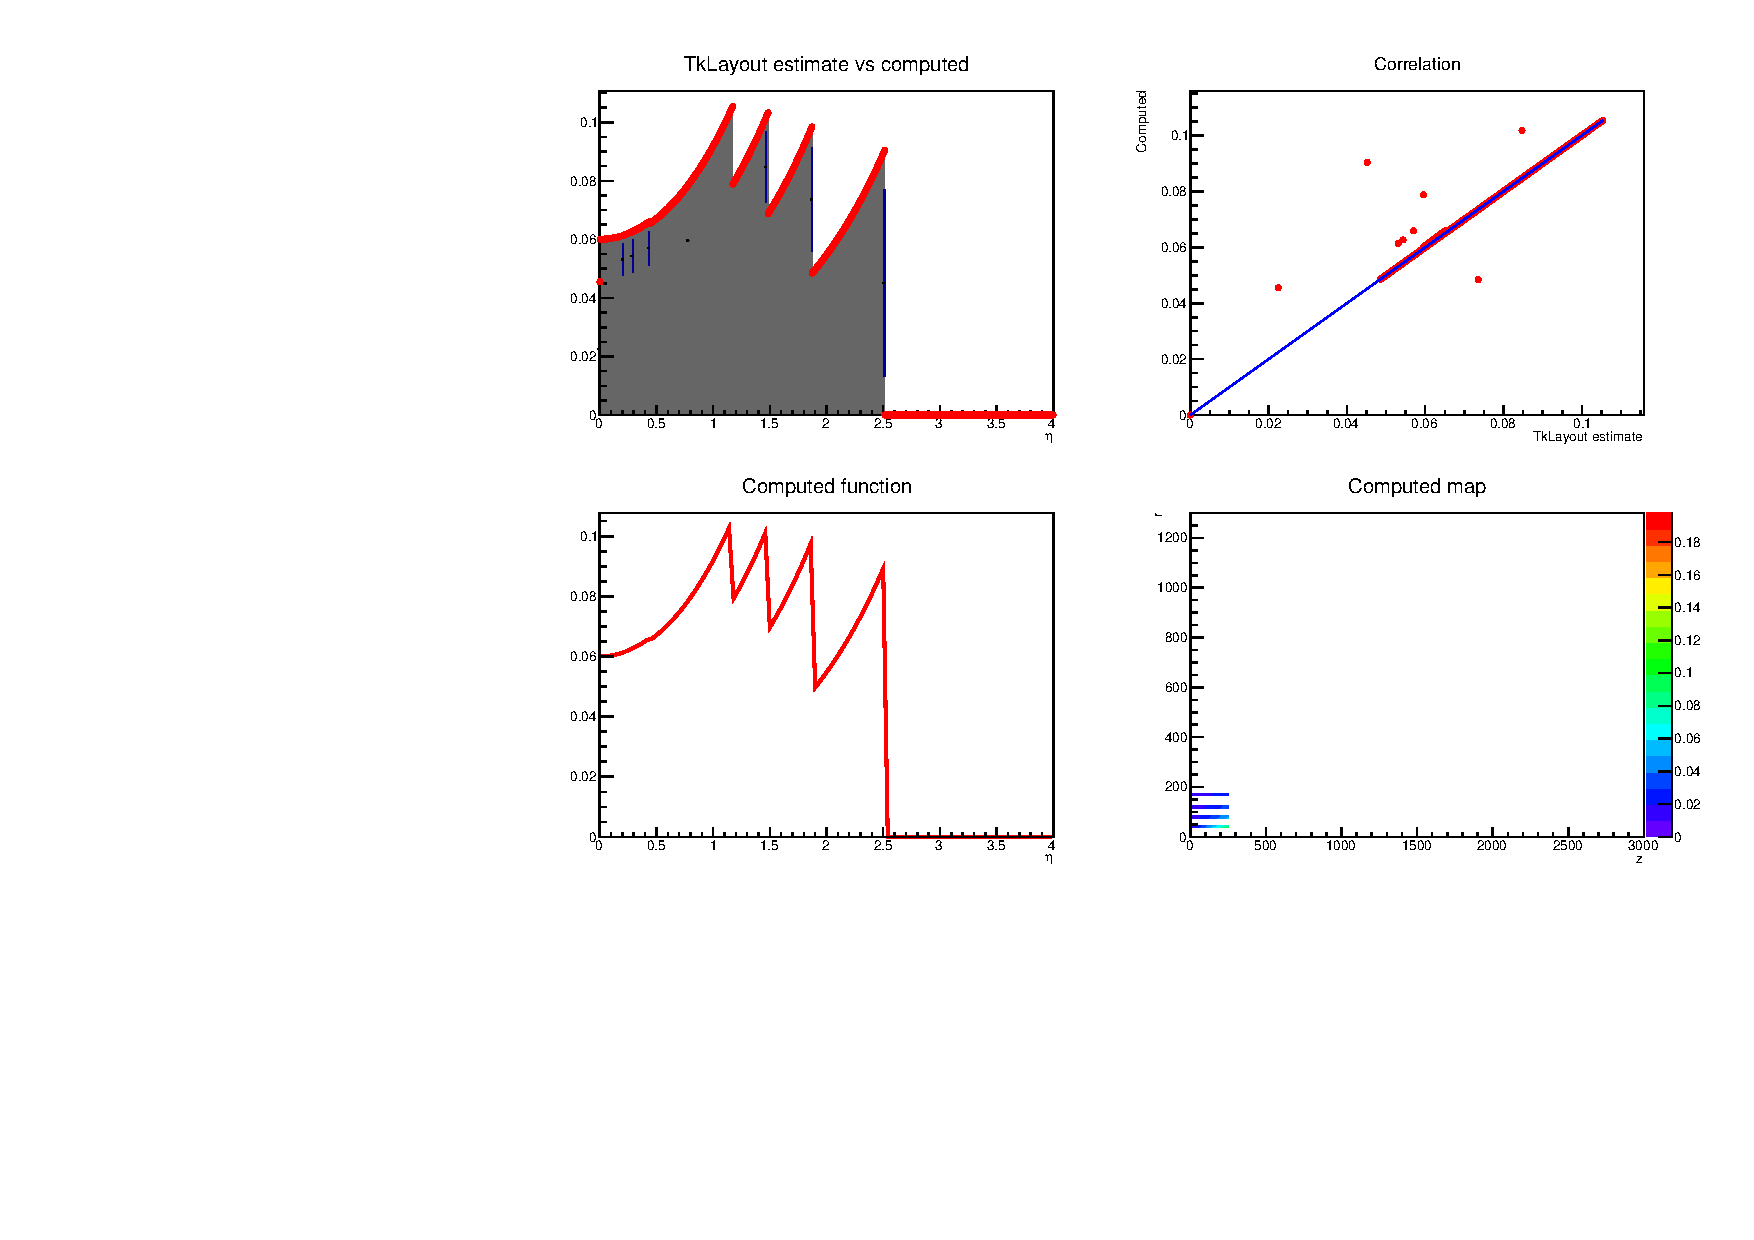
\includegraphics[width=9cm]{img/test21.pdf}
  \end{center}
\end{frame}

\begin{frame}
  \begin{block}{Test22}
    \alert{$100 g/m$} of \emph{Cu} in the modules of layer 1 of barrel
    \begin{itemize}
    \item \alert{service} false
    \end{itemize}
  \end{block}
  \begin{center}
    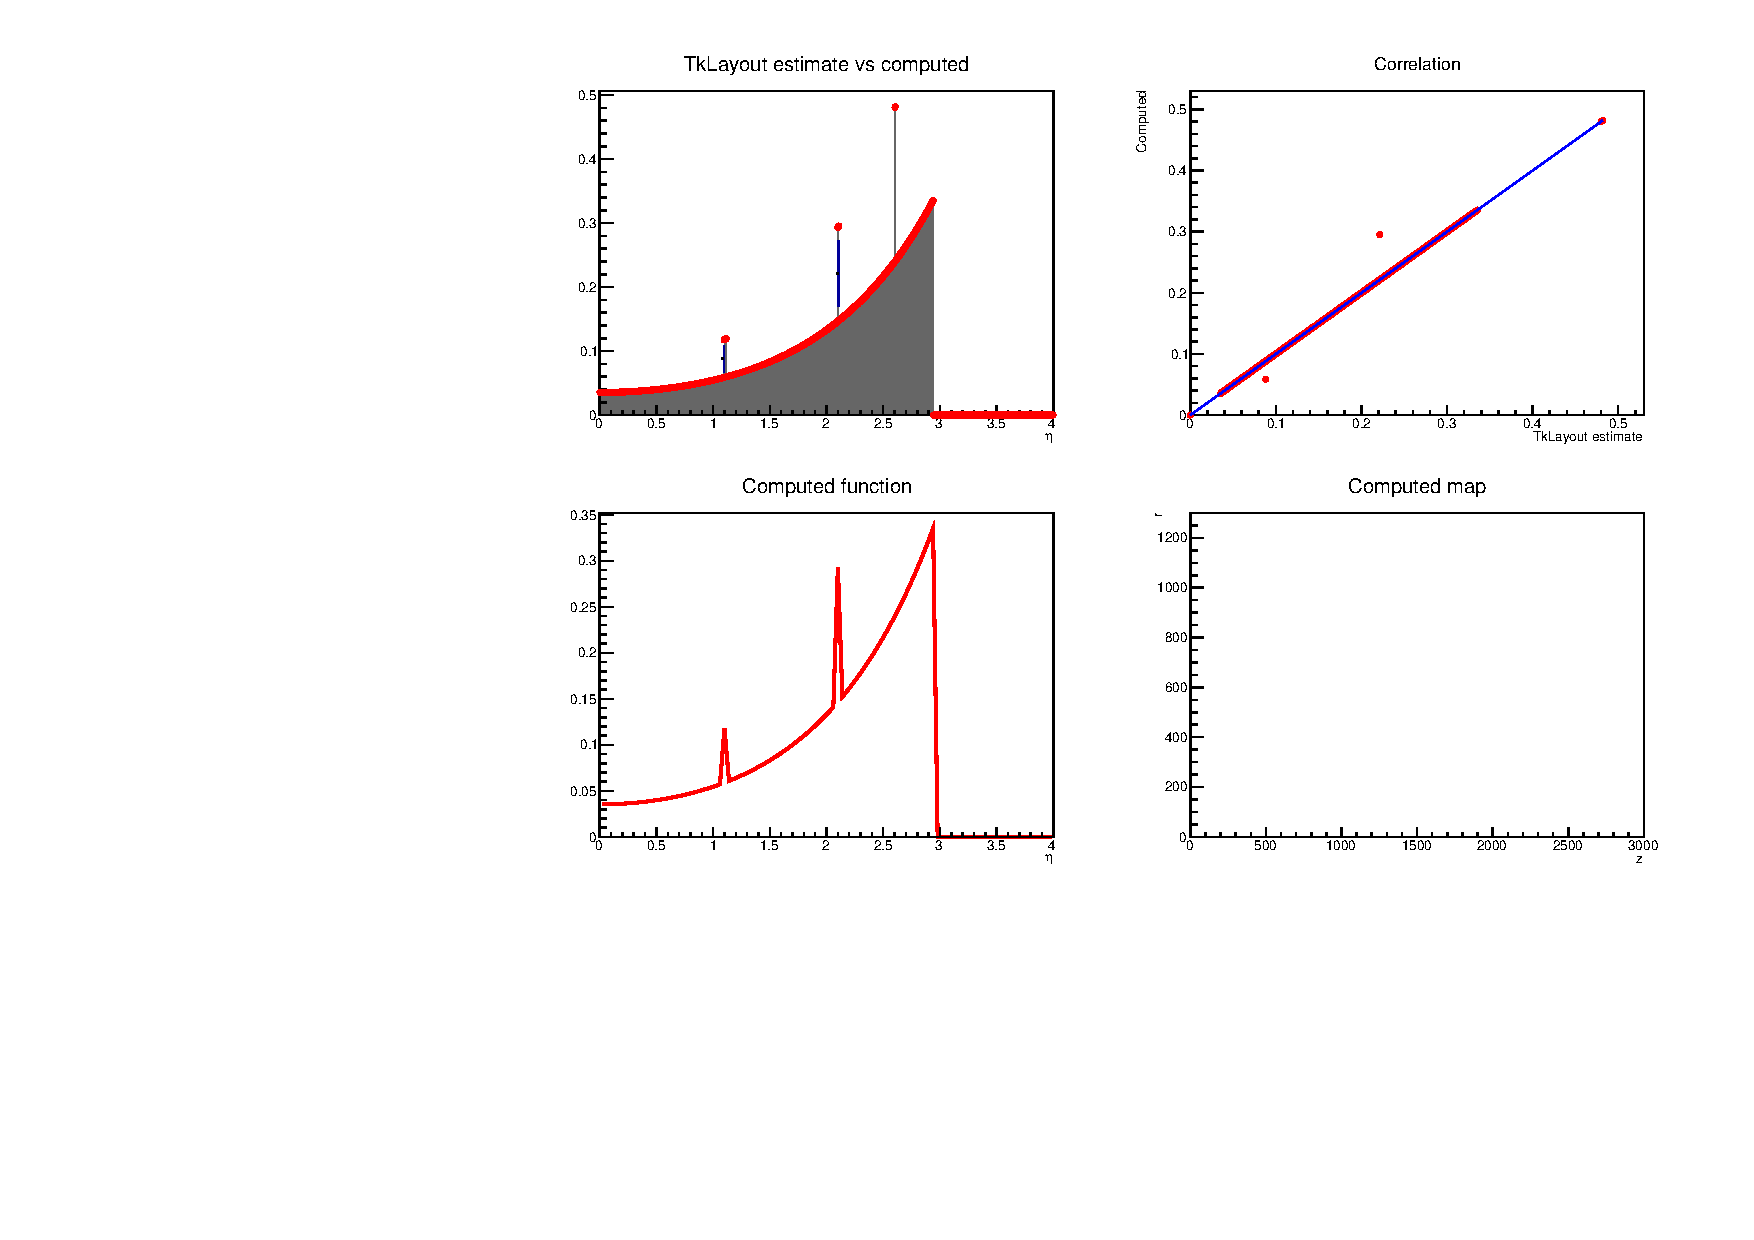
\includegraphics[width=9cm]{img/test22.pdf}
  \end{center}
\end{frame}

\begin{frame}
  \begin{block}{Test22d}
    \alert{$100 g/m$} of \emph{Cu} in the modules of disk 1 of endcap
    \begin{itemize}
    \item \alert{service} false
    \item the second peak is because modules overlaps
    \end{itemize}
  \end{block}
  \begin{center}
    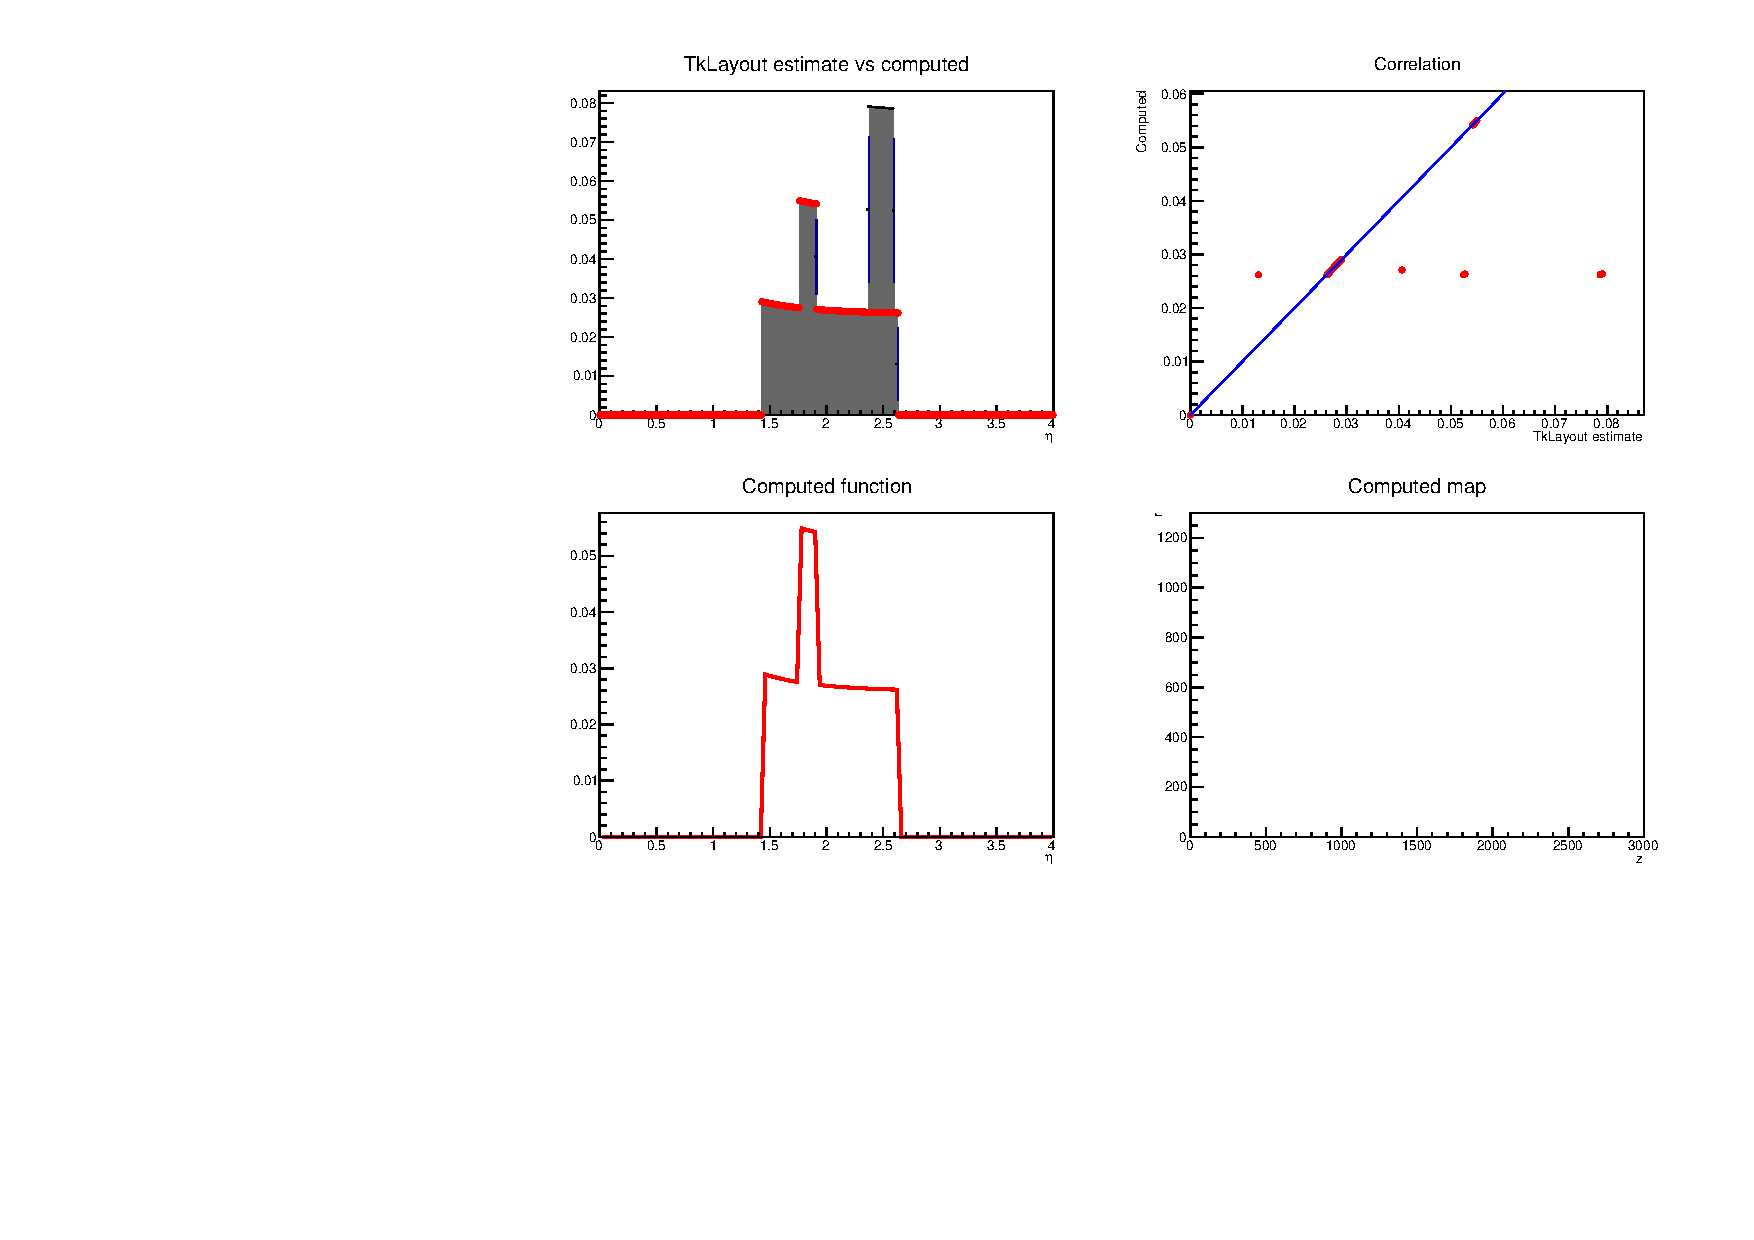
\includegraphics[width=9cm]{img/test22d.pdf}
  \end{center}
\end{frame}

\begin{frame}
  \begin{block}{Test23}
    \alert{$0.1 mm$} of \emph{Cu} in the modules of layer 1 of barrel
    \begin{itemize}
    \item \alert{service} false
    \end{itemize}
  \end{block}
  \begin{center}
    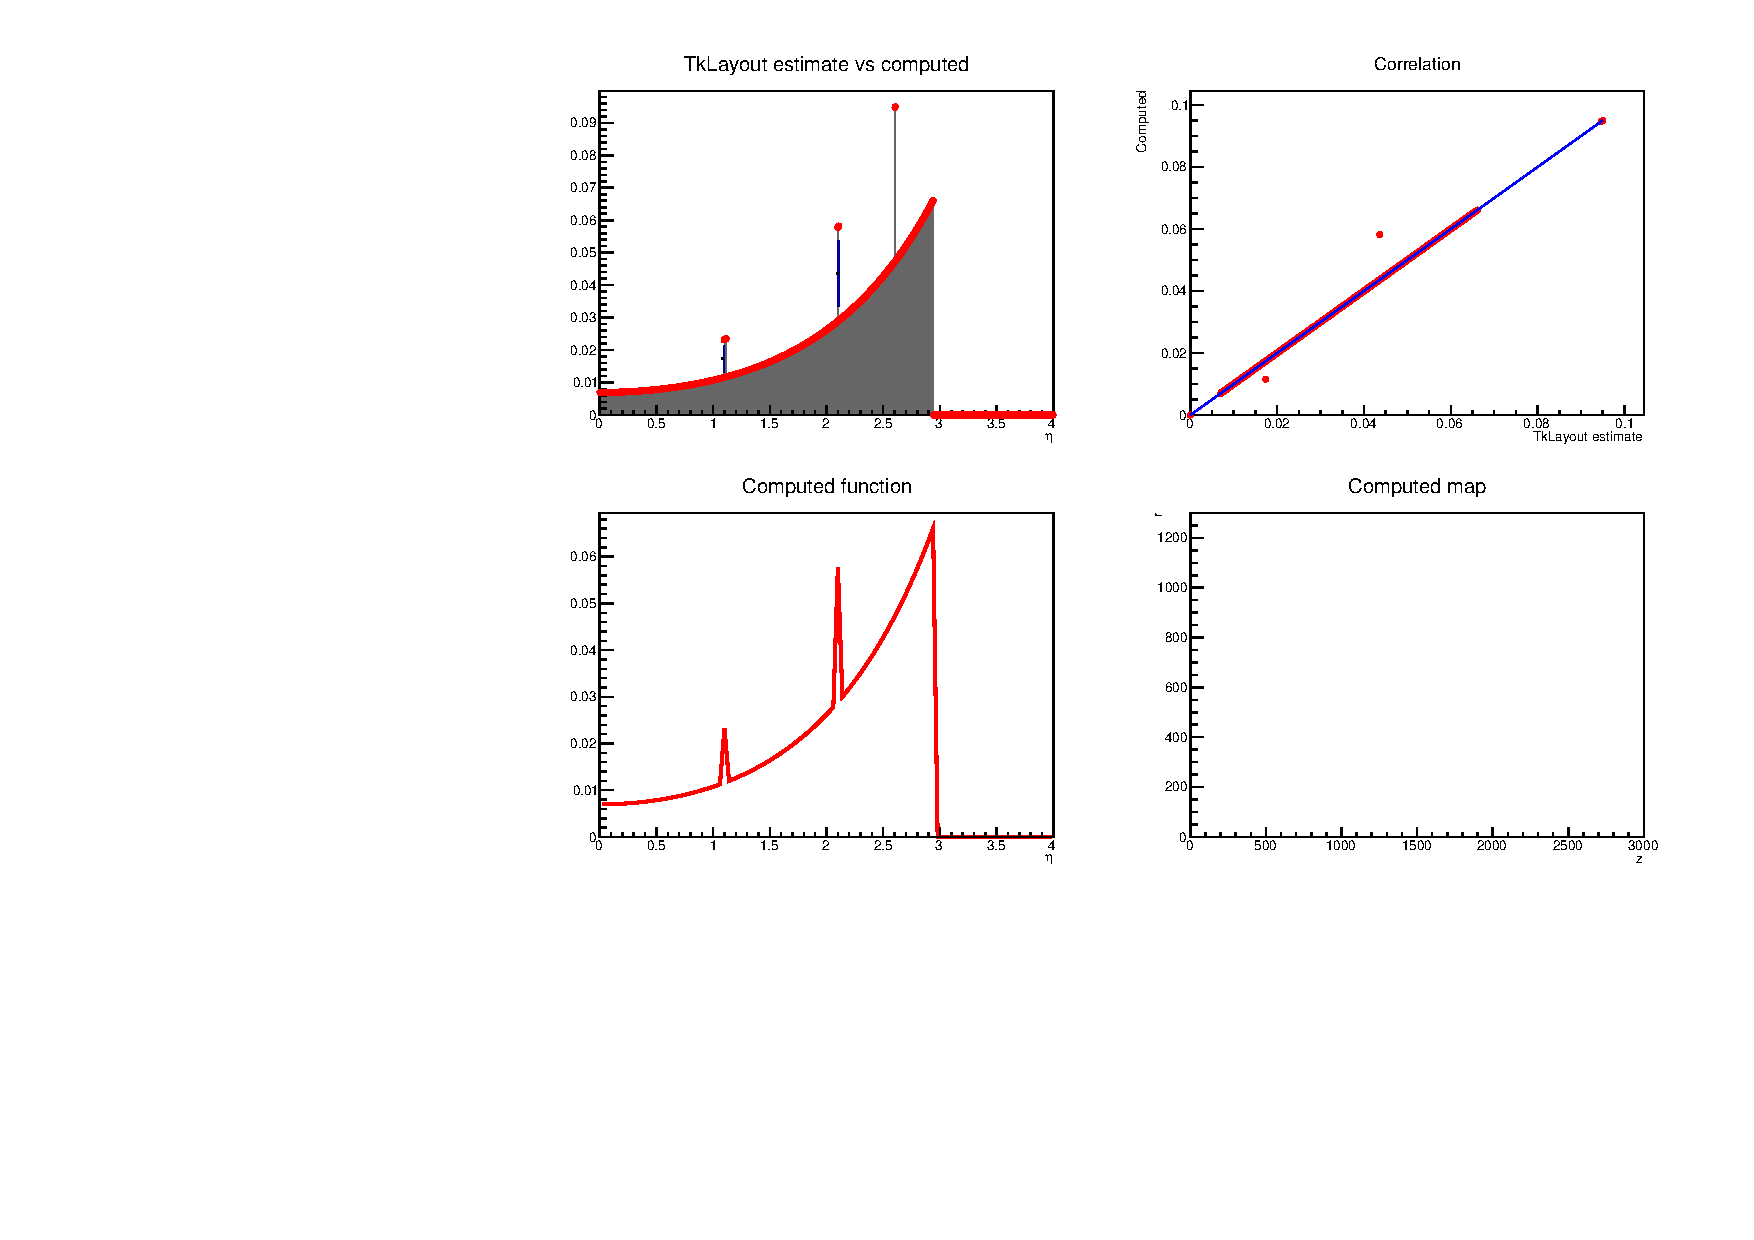
\includegraphics[width=9cm]{img/test23.pdf}
  \end{center}
\end{frame}

\begin{frame}
  \begin{block}{Test23d}
    \alert{$0.1 g/m$} of \emph{Cu} in the modules of layer 1 of barrel
    \begin{itemize}
    \item \alert{service} false
    \item the second peak is because modules overlaps
    \end{itemize}
  \end{block}
  \begin{center}
    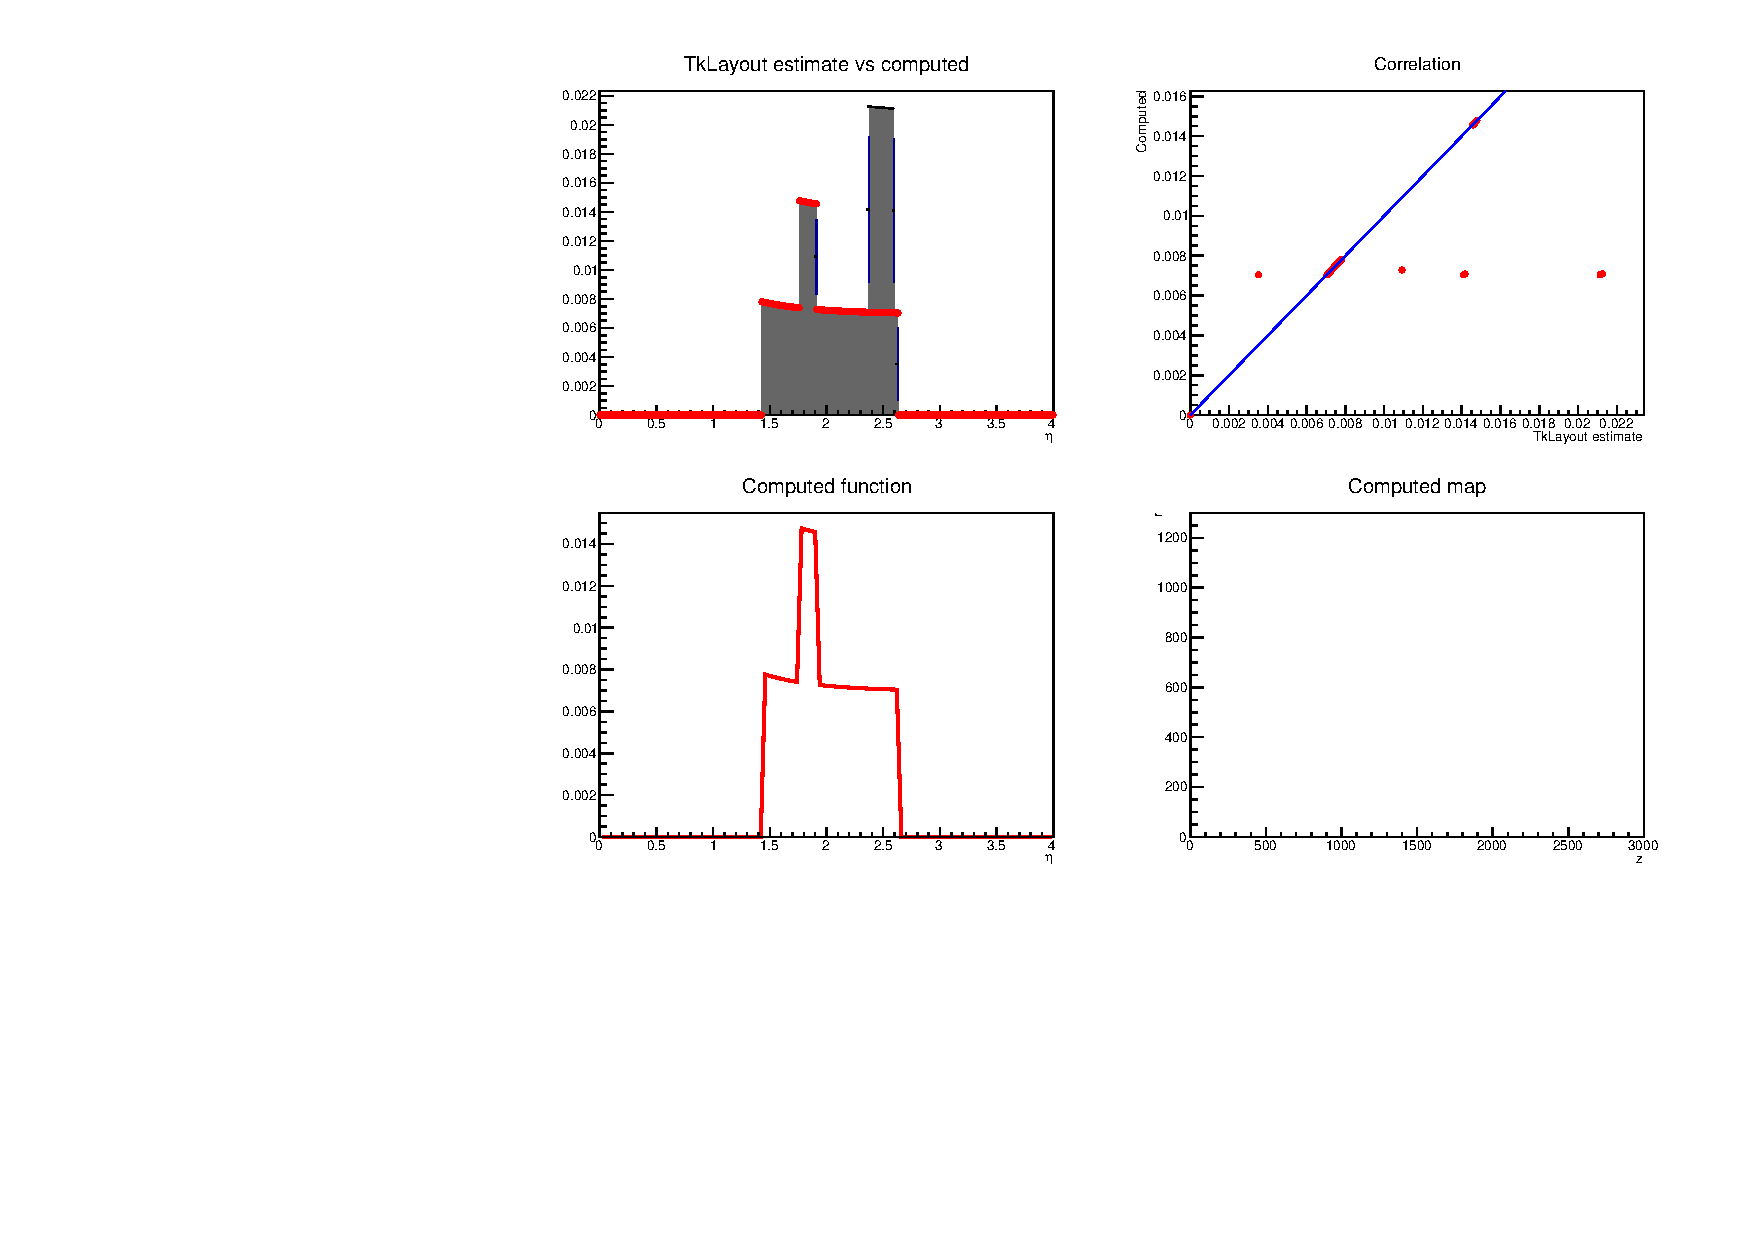
\includegraphics[width=9cm]{img/test23d.pdf}
  \end{center}
\end{frame}

\begin{frame}
  \begin{block}{Test24}
    \alert{$10 g$} of \emph{Cu} in the modules of layer 1 of barrel
    \begin{itemize}
    \item \alert{service} false
    \end{itemize}
  \end{block}
  \begin{center}
    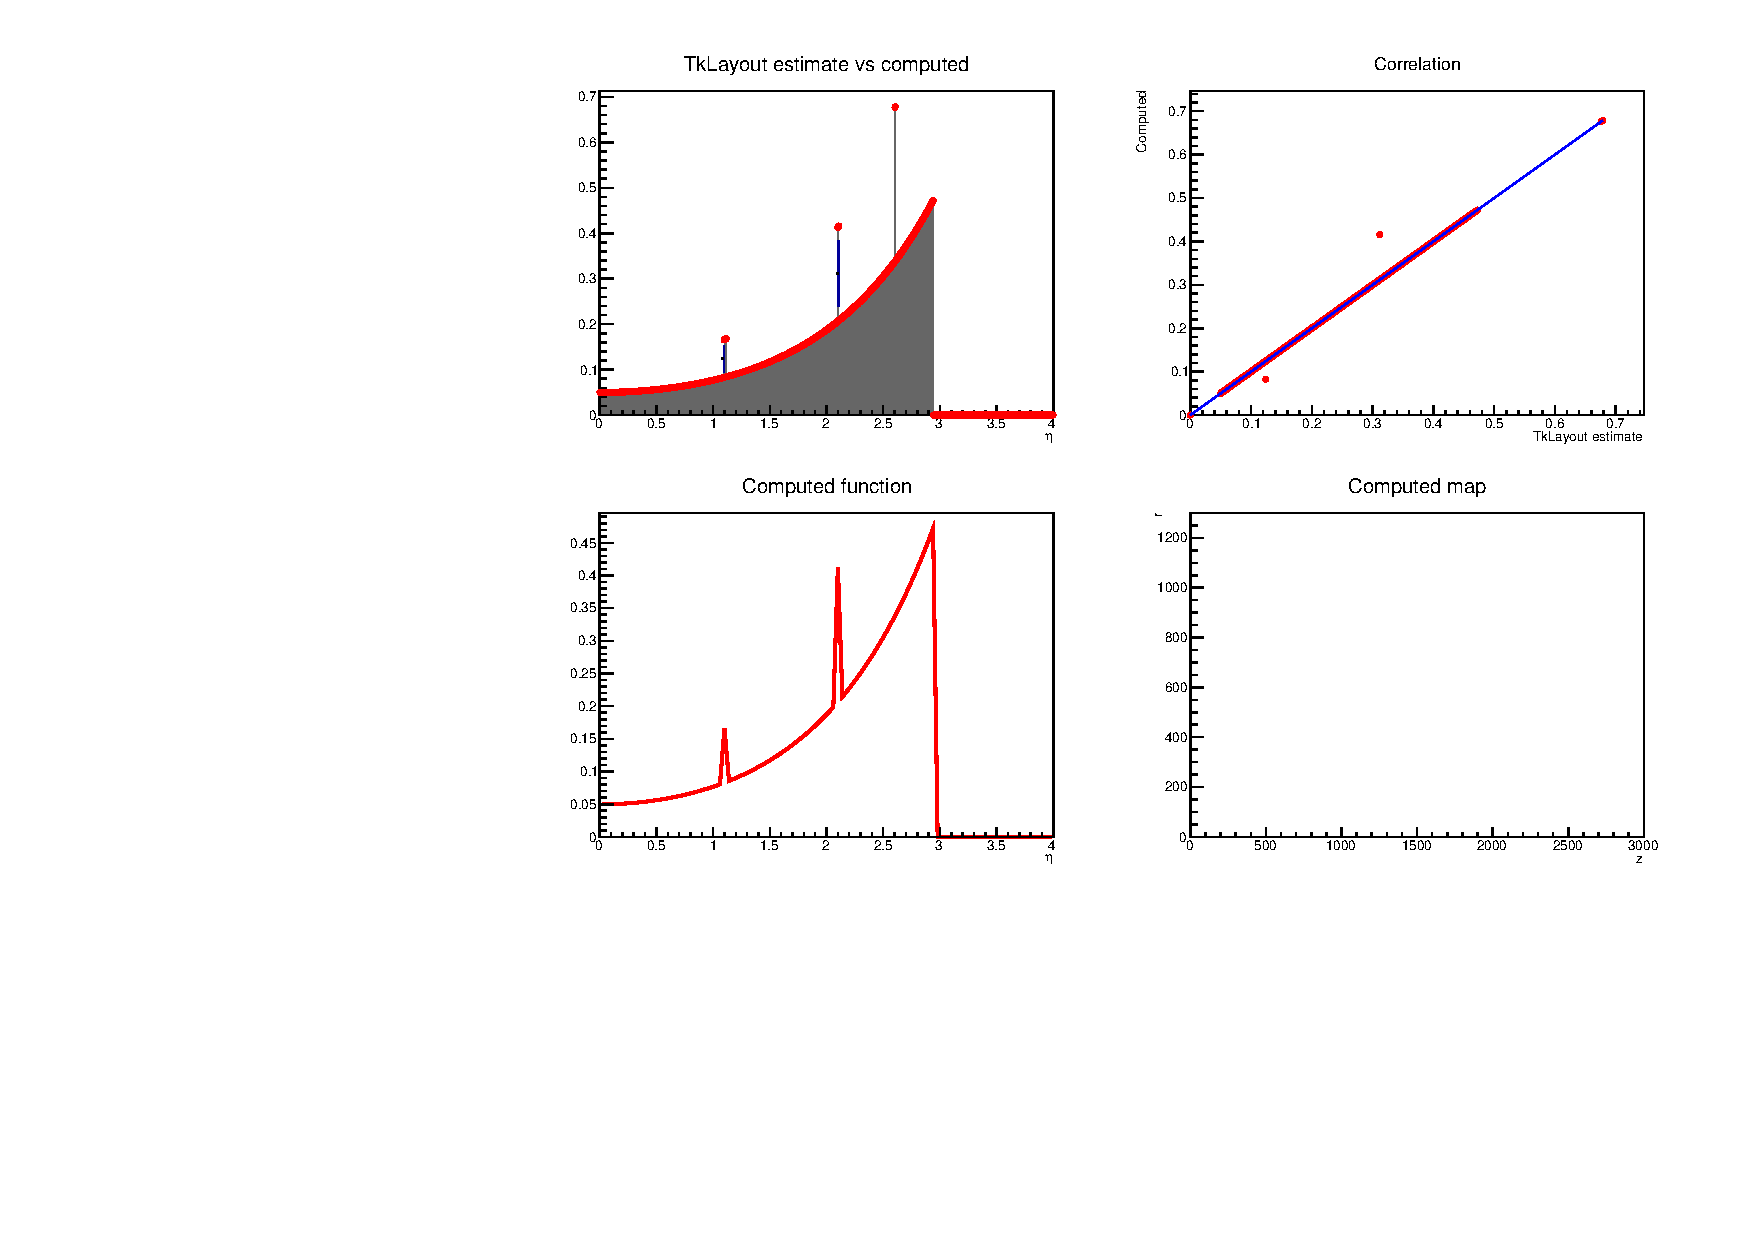
\includegraphics[width=9cm]{img/test24.pdf}
  \end{center}
\end{frame}

\begin{frame}
  \begin{block}{Test24d}
    \alert{$10 g$} of \emph{Cu} in the modules of layer 1 of barrel
    \begin{itemize}
    \item \alert{service} false
    \item the second peak is because modules overlaps
    \end{itemize}
  \end{block}
  \begin{center}
    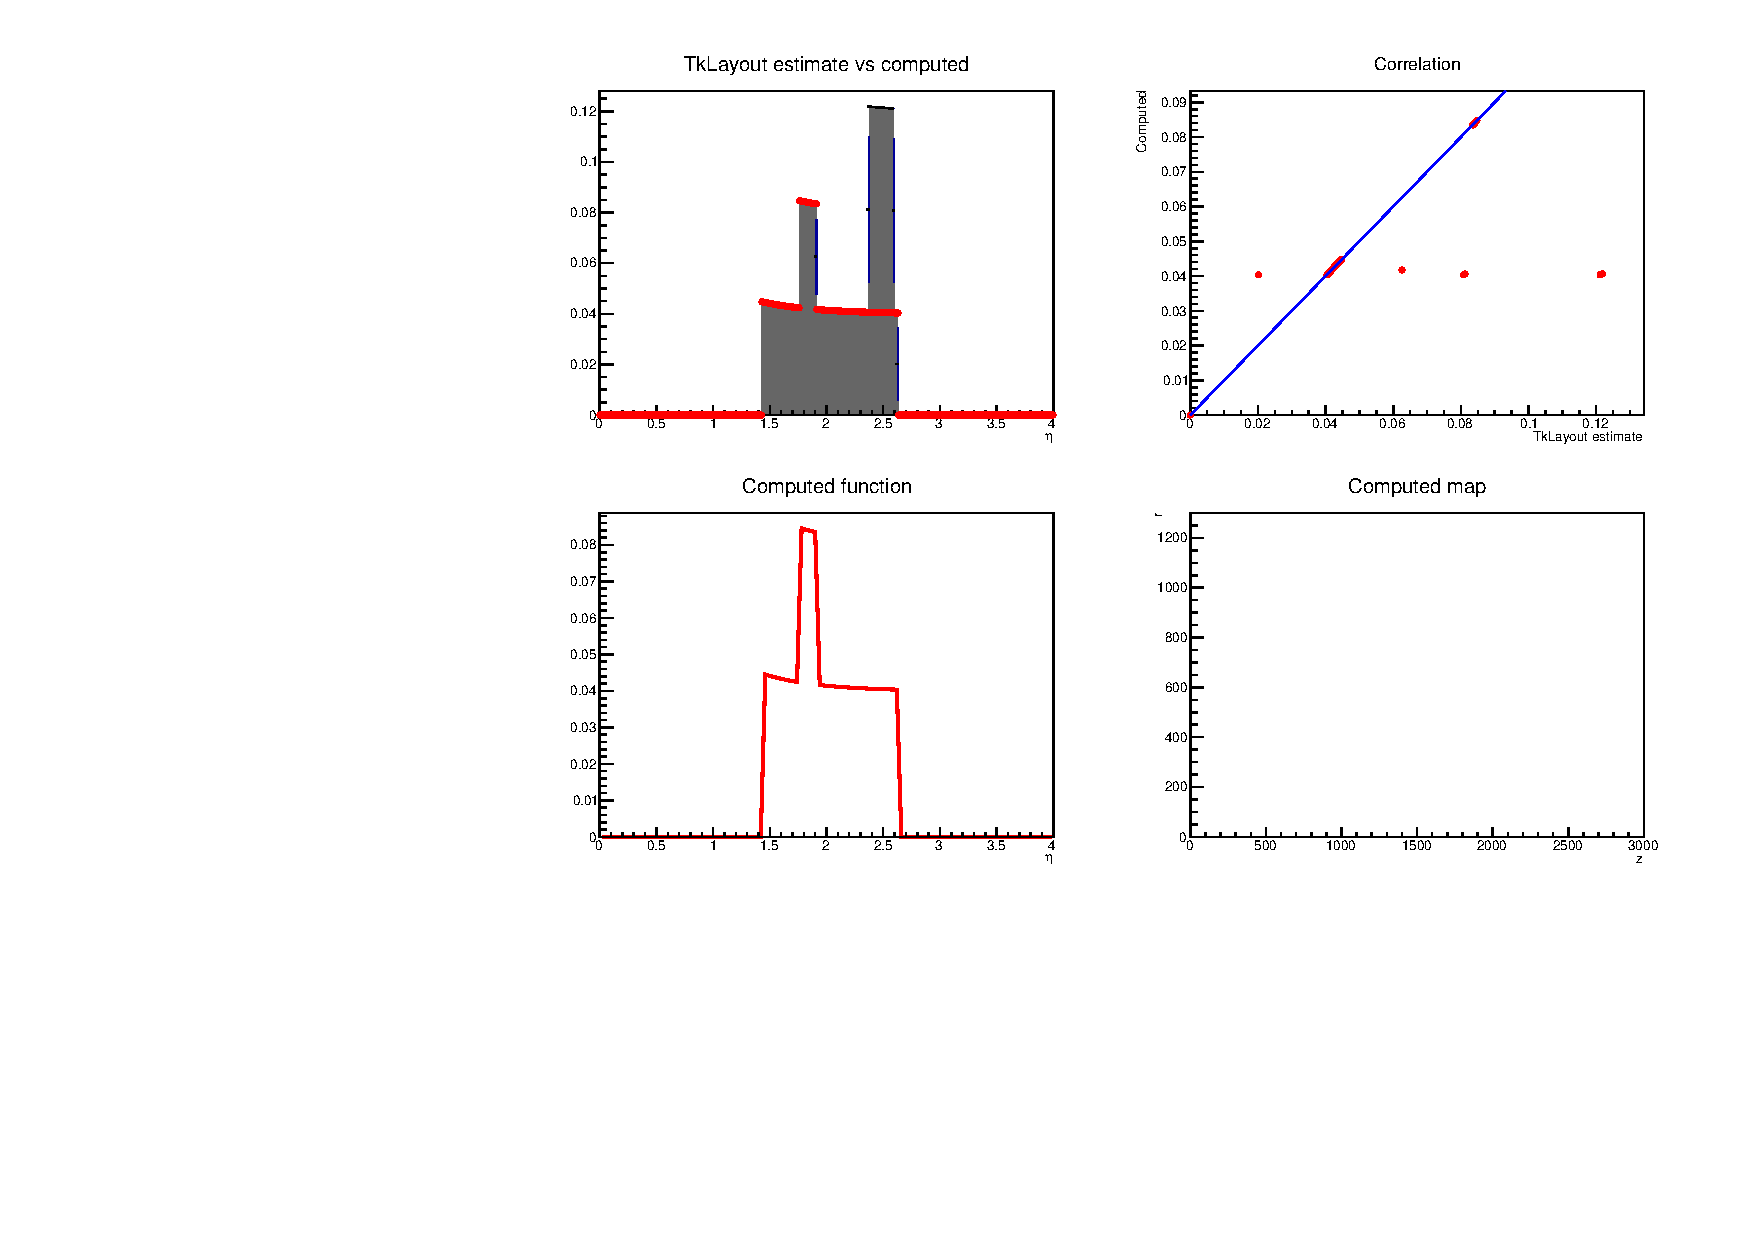
\includegraphics[width=9cm]{img/test24d.pdf}
  \end{center}
\end{frame}

\begin{frame}[fragile]{Expected elements}
  \begin{block}{\svntitlesize test1a}
    \svnbodysize
    \verbatiminput{csv/test1a.csv}
  \end{block}
  \begin{block}{\svntitlesize test1b}
    \svnbodysize
    \verbatiminput{csv/test1b.csv}
  \end{block}
  \begin{block}{\svntitlesize test1c}
    \svnbodysize
    \verbatiminput{csv/test1c.csv}
  \end{block}
  \begin{block}{\svntitlesize test1d}
    \svnbodysize
    \verbatiminput{csv/test1d.csv}
  \end{block}
\end{frame}

\begin{frame}[fragile]
  \begin{block}{\svntitlesize test2}
    \svnbodysize
    \verbatiminput{csv/test2.csv}
  \end{block}
  \begin{block}{\svntitlesize test3}
    \svnbodysize
    \verbatiminput{csv/test3.csv}
  \end{block}
  \begin{block}{\svntitlesize test3bis}
    \svnbodysize
    \verbatiminput{csv/test3bis.csv}
  \end{block}
\end{frame}

\begin{frame}[fragile]
  \begin{block}{\svntitlesize test3ter}
    \svnbodysize
    \verbatiminput{csv/test3ter.csv}
  \end{block}
  \begin{block}{\svntitlesize test3quater}
    \svnbodysize
    \verbatiminput{csv/test3quater.csv}
  \end{block}
  \begin{block}{\svntitlesize test4}
    \svnbodysize
    \verbatiminput{csv/test4.csv}
  \end{block}
  \begin{block}{\svntitlesize test5}
    \svnbodysize
    \verbatiminput{csv/test5.csv}
  \end{block}
\end{frame}

\begin{frame}[fragile]
  \begin{block}{\svntitlesize test6}
    \svnbodysize
    \verbatiminput{csv/test6.csv}
  \end{block}
  \begin{block}{\svntitlesize test6bis}
    \svnbodysize
    \verbatiminput{csv/test6bis.csv}
  \end{block}
  \begin{block}{\svntitlesize test7}
    \svnbodysize
    \verbatiminput{csv/test7.csv}
  \end{block}
\end{frame}

\begin{frame}[fragile]
  \begin{block}{\svntitlesize test8}
    \svnbodysize
    \verbatiminput{csv/test8.csv}
  \end{block}
  \begin{block}{\svntitlesize test9}
    \svnbodysize
    \verbatiminput{csv/test9.csv}
  \end{block}
  \begin{block}{\svntitlesize test10}
    \svnbodysize
    \verbatiminput{csv/test10.csv}
  \end{block}
  \begin{block}{\svntitlesize test10bis}
    \svnbodysize
    \verbatiminput{csv/test10.csv}
  \end{block}
\end{frame}

\begin{frame}[fragile]
  \begin{block}{\svntitlesize test10ter}
    \svnbodysize
    \verbatiminput{csv/test10.csv}
  \end{block}
  \begin{block}{\svntitlesize test11}
    \svnbodysize
    \verbatiminput{csv/test11.csv}
  \end{block}
  \begin{block}{\svntitlesize test11bis}
    \svnbodysize
    \verbatiminput{csv/test11bis.csv}
  \end{block}
\end{frame}

\begin{frame}[fragile]
  \begin{block}{\svntitlesize test12bis}
    \svnbodysize
    \verbatiminput{csv/test12bis.csv}
  \end{block}
\end{frame}

\begin{frame}[fragile]
  \begin{block}{\svntitlesize test13}
    \svnbodysize
    \verbatiminput{csv/test13.csv}
  \end{block}
\end{frame}

\begin{frame}[fragile]
  %% \begin{block}{\svntitlesize test13bis}
  %%   \svnbodysize
  %%   \verbatiminput{csv/test13bis.csv}
  %% \end{block}
  \begin{block}{\svntitlesize test13b}
    \svnbodysize
    \verbatiminput{csv/test13b.csv}
  \end{block}
\end{frame}

\begin{frame}[fragile]
  \begin{block}{\svntitlesize test14}
    \svnbodysize
    \verbatiminput{csv/test14.csv}
  \end{block}
\end{frame}

\begin{frame}[fragile]
  \begin{block}{\svntitlesize test15}
    \svnbodysize
    \verbatiminput{csv/test15.csv}
  \end{block}
\end{frame}

\begin{frame}[fragile]
  \begin{block}{\svntitlesize test15bis}
    \svnbodysize
    \verbatiminput{csv/test15bis.csv}
  \end{block}
\end{frame}

\begin{frame}[fragile]
  \begin{block}{\svntitlesize test16}
    \svnbodysize
    \verbatiminput{csv/test16.csv}
  \end{block}
\end{frame}

\begin{frame}[fragile]
  \begin{block}{\svntitlesize test17}
    \svnbodysize
    \verbatiminput{csv/test17.csv}
  \end{block}
\end{frame}

\begin{frame}[fragile]
  \begin{block}{\svntitlesize test18}
    \svnbodysize
    \verbatiminput{csv/test18.csv}
  \end{block}
  \begin{block}{\svntitlesize test18bis}
    \svnbodysize
    \verbatiminput{csv/test18bis.csv}
  \end{block}
  \begin{block}{\svntitlesize test19}
    \svnbodysize
    \verbatiminput{csv/test19.csv}
  \end{block}
\end{frame}

\begin{frame}[fragile]
  \begin{block}{\svntitlesize test19bis}
    \svnbodysize
    \verbatiminput{csv/test19bis.csv}
  \end{block}
  \begin{block}{\svntitlesize test20}
    \svnbodysize
    \verbatiminput{csv/test20.csv}
  \end{block}
\end{frame}

\begin{frame}[fragile]
  \begin{block}{\svntitlesize test21}
    \svnbodysize
    \verbatiminput{csv/test21.csv}
  \end{block}
\end{frame}

\begin{frame}[fragile]
  \begin{block}{\svntitlesize test22}
    \svnbodysize
    \verbatiminput{csv/test22.csv}
  \end{block}
  \begin{block}{\svntitlesize test22d}
    \svnbodysize
    \verbatiminput{csv/test22d.csv}
  \end{block}
\end{frame}

\begin{frame}[fragile]
  \begin{block}{\svntitlesize test23}
    \svnbodysize
    \verbatiminput{csv/test23.csv}
  \end{block}
  \begin{block}{\svntitlesize test23d}
    \svnbodysize
    \verbatiminput{csv/test23d.csv}
  \end{block}
\end{frame}

\begin{frame}[fragile]
  \begin{block}{\svntitlesize test24}
    \svnbodysize
    \verbatiminput{csv/test24.csv}
  \end{block}
  \begin{block}{\svntitlesize test24d}
    \svnbodysize
    \verbatiminput{csv/test24d.csv}
  \end{block}
\end{frame}

\end{document}
